% Options for packages loaded elsewhere
\PassOptionsToPackage{unicode}{hyperref}
\PassOptionsToPackage{hyphens}{url}
%
\documentclass[
  12pt,
  a4paper,
  twoside]{article}
\usepackage{amsmath,amssymb}
\usepackage{lmodern}
\usepackage{iftex}
\ifPDFTeX
  \usepackage[T1]{fontenc}
  \usepackage[utf8]{inputenc}
  \usepackage{textcomp} % provide euro and other symbols
\else % if luatex or xetex
  \usepackage{unicode-math}
  \defaultfontfeatures{Scale=MatchLowercase}
  \defaultfontfeatures[\rmfamily]{Ligatures=TeX,Scale=1}
\fi
% Use upquote if available, for straight quotes in verbatim environments
\IfFileExists{upquote.sty}{\usepackage{upquote}}{}
\IfFileExists{microtype.sty}{% use microtype if available
  \usepackage[]{microtype}
  \UseMicrotypeSet[protrusion]{basicmath} % disable protrusion for tt fonts
}{}
\makeatletter
\@ifundefined{KOMAClassName}{% if non-KOMA class
  \IfFileExists{parskip.sty}{%
    \usepackage{parskip}
  }{% else
    \setlength{\parindent}{0pt}
    \setlength{\parskip}{6pt plus 2pt minus 1pt}}
}{% if KOMA class
  \KOMAoptions{parskip=half}}
\makeatother
\usepackage{xcolor}
\IfFileExists{xurl.sty}{\usepackage{xurl}}{} % add URL line breaks if available
\IfFileExists{bookmark.sty}{\usepackage{bookmark}}{\usepackage{hyperref}}
\hypersetup{
  pdftitle={MATH1049 Linear Algebra II lecture notes},
  pdfauthor={Ján Špakula},
  hidelinks,
  pdfcreator={LaTeX via pandoc}}
\urlstyle{same} % disable monospaced font for URLs
\usepackage[a4paper,top=1in,bottom=1in,left=1.2in,right=0.8in]{geometry}
\usepackage{longtable,booktabs,array}
\usepackage{calc} % for calculating minipage widths
% Correct order of tables after \paragraph or \subparagraph
\usepackage{etoolbox}
\makeatletter
\patchcmd\longtable{\par}{\if@noskipsec\mbox{}\fi\par}{}{}
\makeatother
% Allow footnotes in longtable head/foot
\IfFileExists{footnotehyper.sty}{\usepackage{footnotehyper}}{\usepackage{footnote}}
\makesavenoteenv{longtable}
\usepackage{graphicx}
\makeatletter
\def\maxwidth{\ifdim\Gin@nat@width>\linewidth\linewidth\else\Gin@nat@width\fi}
\def\maxheight{\ifdim\Gin@nat@height>\textheight\textheight\else\Gin@nat@height\fi}
\makeatother
% Scale images if necessary, so that they will not overflow the page
% margins by default, and it is still possible to overwrite the defaults
% using explicit options in \includegraphics[width, height, ...]{}
\setkeys{Gin}{width=\maxwidth,height=\maxheight,keepaspectratio}
% Set default figure placement to htbp
\makeatletter
\def\fps@figure{htbp}
\makeatother
\setlength{\emergencystretch}{3em} % prevent overfull lines
\providecommand{\tightlist}{%
  \setlength{\itemsep}{0pt}\setlength{\parskip}{0pt}}
\setcounter{secnumdepth}{5}
\usepackage{xcolor}
\usepackage{mathptmx}
\usepackage{extarrows}
\usepackage{mathdots}

% weird underlining
\usepackage[normalem]{ulem}

% temporary fix for "Missing number, treated as zero." for \linethickness
% apparently pandoc problem, Dec 2019
\renewcommand{\linethickness}{0.05em}

% headers
\usepackage{fancyhdr}
\fancyhead{}
\fancyhead[LE,RO]{\thepage}
\fancyhead[C]{\leftmark}
\fancyfoot{}
\renewcommand{\headrulewidth}{0pt}
\renewcommand{\footrulewidth}{0pt}
\pagestyle{fancy}

% fix how green looks in pdf
\definecolor{green}{rgb}{0,0.5,0}

% want non-bookdown thm/defn numbering
%  (this will of course make it work in latex, but need thms.R and some hacks to make it work in html)

%%% theorem styles (amsthm) --
\usepackage{amsthm}
\theoremstyle{plain}    
 \newtheorem{theorem}{Theorem}[section]
 \newtheorem{lemma}[theorem]{Lemma}
 \newtheorem{corollary}[theorem]{Corollary}
 \newtheorem{proposition}[theorem]{Proposition}
% \newtheorem{conjecture}[theorem]{Conjecture}  % shouldn't use this, it's used for the 'nasty hack'
\theoremstyle{definition}
 \newtheorem{definition}[theorem]{Definition}
%\theoremstyle{remark}
 \newtheorem{example}[theorem]{Example}
 \newtheorem{exercise}[theorem]{Exercise}
 \newtheorem{remark}[theorem]{Remark}
 \newtheorem{solution}[theorem]{Solution}
\ifLuaTeX
  \usepackage{selnolig}  % disable illegal ligatures
\fi

\title{MATH1049 Linear Algebra II lecture notes}
\author{Ján Špakula}
\date{Spring 2021}

\begin{document}
\maketitle

{
\setcounter{tocdepth}{2}
\tableofcontents
}
\hypertarget{preface}{%
\section*{Preface}\label{preface}}
\addcontentsline{toc}{section}{Preface}

These lecture notes contain more--less verbatim what appears on the (black-- or white--)board during the lectures.

The
colour coding
signifies the following: what is
\textcolor{red}{red}
is being \emph{defined}.
\textcolor{blue}{Blue}
are \emph{named theorems and statements} (these could be referred to by these names). Finally
\textcolor{green}{green}
is used to reference lecture notes of other modules (mostly MATH1048 Linear Algebra I).

\hypertarget{acknowledgement}{%
\subsection*{Acknowledgement}\label{acknowledgement}}
\addcontentsline{toc}{subsection}{Acknowledgement}

For the most part, these notes were designed and written by Dr Bernhard Koeck, and originally typed into \(\text{\LaTeX}\) by the undergraduate student Thomas Blundell--Hunter in summer 2011. They have been regularly updated to reflect the changes in the syllabus. The current version is a complete overhaul of the technical side of the notes, so that they are available also in \texttt{html}.

\newpage

\hypertarget{groups}{%
\section{Groups}\label{groups}}

The \textcolor{red}{cartesian product} \(G\times H\) of two sets \(G\) and \(H\) is defined as the set
\[ G\times H := \{(g,h) \mid g\in G, h\in H\}, \]
consisting of all (ordered) pairs \((g,h)\) where \(g\in G\) and \(h\in H\). For example, \(\mathbb{R}^2 = \mathbb{R}\times \mathbb{R}\).

\csname begin\endcsname{definition}\label{cnj:defn-group}

\begin{enumerate}
\def\labelenumi{(\alph{enumi})}
\item
  A \textcolor{red}{binary operation} on a set \(G\) is a function \(G\times G\to G\) (from the cartesian product \(G\times G=\{(a,b)\mid a\in G, b\in G\}\) to \(G\)). We write \(a * b\) (or \(ab\), or \(a\circ b\), or \(a+b\)) for the image of the pair \((a,b)\in G\times G\) in \(G\) under this function.
\item
  A \textcolor{red}{group} is a set \(G\) together with a binary operation \(G\times G\to G\), \((a,b)\mapsto a*b\) (which we usually refer to as ``group operation'', or ``group multiplication'', or just ``multiplication'') such that the following axioms are satisfied:

  \begin{enumerate}
  \def\labelenumii{(\roman{enumii})}
  \item
    \emph{Associativity}: For all \(a,b,c\in G\), we have \((a*b)*c = a*(b*c)\) in \(G\).
  \item
    \emph{Existence of the identity (or neutral) element}: There exists \(e\in G\), such that for all \(a\in G\) we have \(e*a=a=a*e\).
  \item
    \emph{Existence of the right inverse}: For every \(a\in G\) there exists \(b\in G\) such that \(a*b=e\).
  \end{enumerate}
\item
  A group is called \textcolor{red}{abelian} (or \textcolor{red}{commutative}), if for all \(a,b\in G\) we have \(a*b=b*a\).
\item
  A group is called \textcolor{red}{finite} if \(G\) has only finitely many elements; in this case its cardinality \(|G|\) is called the \textcolor{red}{order} of \(G\).
\end{enumerate}

\csname end\endcsname{definition}

\csname begin\endcsname{example}\label{cnj:expl-groups}

\begin{enumerate}
\def\labelenumi{(\alph{enumi})}
\item
  The usual addition \(\mathbb{N}\times\mathbb{N}\to\mathbb{N}\), \((m,n)\mapsto m+n\), defines a binary operation on \(\mathbb{N}\) (and so does multiplication), but subtraction does not, because for instance \(2-3=-1\not\in\mathbb{N}\).
\item
  The sets \(\mathbb{Z}, \mathbb{Q}, \mathbb{R}\) and \(\mathbb{C}\) together with addition as the binary operation are abelian groups. The sets \(\mathbb{Q}^*:=\mathbb{Q}\setminus\{0\}\), \(\mathbb{R}^*:=\mathbb{R}\setminus\{0\}\) and \(\mathbb{C}^*:=\mathbb{C}\setminus\{0\}\) together with multiplication as the binary operation are abelian groups.
\item
  The set \(\mathbb{N}\) with addition is not a group, because, for example, there doesn't exist a (right) inverse to \(1\in\mathbb{N}\). (In other words, the equation \(1+ ? =0\) has no solution in \(\mathbb{N}\).)
\item
  For any \(n\in\mathbb{N}\), the set \(\mathbb{R}^n\) together with vector addition is a group. For any \(m,n\in\mathbb{N}\) the set \textcolor{red}{$M_{m\times n}(\mathbb{R})$} of real \(m\)--by--\(n\) matrices together with matrix addition is a group. For every \(n\in \mathbb{N}\), the set \(\mathrm{GL}_n(\mathbb{R})\) of invertible real \((n\times n)\)--matrices together with matrix multiplication is a group, called the \emph{general linear group}. If \(n>1\), \(\mathrm{GL}_n(\mathbb{R})\) is not abelian: e.g.
  \[
  \begin{pmatrix}1&1\\0&1\end{pmatrix}\cdot
  \begin{pmatrix}1&0\\1&1\end{pmatrix} =
  \begin{pmatrix}2&1\\1&1\end{pmatrix}, \quad \text{but} \quad
  \begin{pmatrix}1&0\\1&1\end{pmatrix}\cdot
  \begin{pmatrix}1&1\\0&1\end{pmatrix} =
  \begin{pmatrix}1&1\\1&2\end{pmatrix}.
  \]
\end{enumerate}

\csname end\endcsname{example}

\csname begin\endcsname{proposition}\label{cnj:prop-groups-enhancing-axioms}
Let \(G\) be a group. Then:

\begin{enumerate}
\def\labelenumi{(\alph{enumi})}
\item
  There exists precisely one identity element in \(G\).
\item
  For every \(a\in G\) there exists precisely one right inverse (call it \(b\)) to \(a\), and this \(b\) is also a left inverse of \(a\) (meaning that we also have \(b*a=e\)). We write \(a^{-1}\) for this inverse of \(a\) (or \(-a\) if the group operation is ``\(+\)'').
\end{enumerate}

\csname end\endcsname{proposition}

\begin{proof}
\iffalse{} {Proof. } \fi{}(a) Suppose \(e\) and \(e'\) are two identity elements in \(G\).\\
\(\implies\) \(e*e' = e\) \hfill~{(because \(e'\) is an identity element)}\\
\hspace*{0.333em}\hspace*{0.333em}\hspace*{0.333em}and \(e*e' = e'\) \hfill~{(because \(e\) is an identity element)}\\
\(\implies\) \(e=e'\).

\(\)(b) Let \(b\) be a right inverse of \(a\), and let \(c\) be a right inverse of \(b\).\\
\(\implies\) \(a*(b*c) = a*e\) \hfill~{(because \(c\) is a right inverse of \(b\))}\\
\hspace*{0.333em}\hspace*{0.333em}\hspace*{0.333em}\hspace*{0.333em}\hspace*{0.333em}\hspace*{0.333em}\hspace*{0.333em}\hspace*{0.333em}\hspace*{0.333em} \(= a\) \hfill~{(because \(e\) is the identity element)}\\
\hspace*{0.333em}\hspace*{0.333em}\hspace*{0.333em}and \(a*(b*c) = (a*b)*c\) \hfill~{(by associativity)}\\
\hspace*{0.333em}\hspace*{0.333em}\hspace*{0.333em}\hspace*{0.333em}\hspace*{0.333em}\hspace*{0.333em}\hspace*{0.333em}\hspace*{0.333em}\hspace*{0.333em} \(= e*c\) \hfill~{(because \(b\) is a right inverse of \(a\))}\\
\hspace*{0.333em}\hspace*{0.333em}\hspace*{0.333em}\hspace*{0.333em}\hspace*{0.333em}\hspace*{0.333em}\hspace*{0.333em}\hspace*{0.333em}\hspace*{0.333em} \(= c\) \hfill~{(because \(e\) is the identity element)}\\
\(\implies\) \(a=c\)\\
\(\implies\) \(b*a = b*c = e\). \hfill~{(because \(c\) is a right inverse of \(b\))}\\
In other words, \(b\) is also a left inverse of \(a\).\\
Suppose that \(b'\) is another right inverse of \(a\).\\
\(\implies\) \(b=b*e=b*(a*b')=(b*a)*b' = e*b' = b'\).\\
(These equalities hold by: definition of \(e\), definition of \(b'\), associativity, the fact we just proved, and by definition of \(e\), respectively.)
\end{proof}

\csname begin\endcsname{proposition}\label{cnj:prop-more-group-props}
Let \(G\) be a group.

\begin{enumerate}
\def\labelenumi{(\alph{enumi})}
\item
  (\emph{Cancellation}) If \(a,b,z\in G\) and \(a*z=b*z\) (or \(z*a=z*b\)), then \(a=b\).
\item
  For all \(a\in G\) both the equation \(a*x=b\) and \(y*a=b\) have a unique solution in \(G\). (Another way to say this: for every \(a\in G\), both the map \(G\to G\), \(x\mapsto a*x\) (called \textcolor{red}{left translation by $a$}) and \(G\to G\), \(y\mapsto y*a\) (called \textcolor{red}{right translation by $a$}) are bijective.)
\item
  For every \(a\in G\) we have \((a^{-1})^{-1}=a\).
\item
  For all \(a,b\in G\) we have \((a*b)^{-1}=b^{-1}*a^{-1}\).
\item
  (\emph{Exponential laws}) For any \(m\in \mathbb{Z}\) and \(a\in G\), we define:
  \[
  {\color{red}{a^m}} :=
  \begin{cases}
  \underbrace{a*a*\cdots*a}_{m\text{ times}} & \text{if }m>0;\\
  e & \text{if }m=0;\\
  (a^{-1})^{|m|} & \text{if }m<0.
  \end{cases}
  \]
  (In additive notation, i.e.~when the group operation is ``+'', we write \textcolor{red}{$ma$} instead of \(a^m\).)\\
  Then for all \(m,n\in\mathbb{Z}\) and \(a\in G\) we have \(a^{m+n}=a^m * a^n\) and \(a^{mn}=(a^m)^n\).\\
  If \(a,b\in G\) \textcolor{red}{commute} (i.e.~\(a*b=b*a\)), then for all \(m\in\mathbb{Z}\) we have \((a*b)^m = a^m*b^m\).
\end{enumerate}

\csname end\endcsname{proposition}

\begin{proof}
\iffalse{} {Proof. } \fi{}(a) Multiply both sides of the equation by \(z^{-1}\).

\begin{enumerate}
\def\labelenumi{(\alph{enumi})}
\setcounter{enumi}{1}
\item
  Proof of the ``another way'': \emph{Injectivity}: use (a).\\
  \emph{Surjectivity}: If \(b\in G\), then \(b*a^{-1}\) is mapped to \(b\) under the right translation by \(a\).
\item
  Both \((a^{-1})^{-1}\) and \(a\) are solutions of the equation \(a^{-1}*x=e\) (see Proposition \ref{cnj:prop-groups-enhancing-axioms} (b)). Now apply (b).
\item
  We have \((a*b)*(b^{-1}*a^{-1}) = a*(b*(b^{-1}*a^{-1})) = a*((b*b^{-1})*a^{-1})\) \(= a*(e*a^{-1})\) \(=a*a^{-1} = e\). \(\implies\) \(b^{-1}*a^{-1}\) is a right inverse to \(a*b\).
\end{enumerate}

\(\)~~~(e) Left as an exercise.
\end{proof}

\csname begin\endcsname{example}\label{cnj:expl-groups-more}

\begin{enumerate}
\def\labelenumi{(\alph{enumi})}
\item
  The \textcolor{red}{group table} of a finite group \(G=\{a_1,a_2,\dots,a_n\}\) is a table like this:
  \[
  \begin{array}{c|ccc}
  \ast & \cdots & a_j & \cdots \\
  \hline
  \vdots & \ddots & \vdots & \\
  a_i & \cdots & a_i*a_j & \cdots\\
  \vdots &  & \vdots & 
  \end{array}
  \]
  The \textcolor{red}{trivial group} is the group with exactly one element, say \(e\). Its group table must be
  \[
  \begin{array}{c|c} * & e \\ \hline e & e\end{array}
  \]
  Any group with two elements, say \(e\) and \(a\), is given by the group table:
  \[
  \begin{array}{c|cc} * & e & a \\ \hline e & e & a \\ a & a & e\end{array}
  \]
  Any group with three elements, say \(e, a\) and \(b\), must have group table:
  \[
  \begin{array}{c|ccc} * & e & a & b \\ \hline e & e & a & b \\
  a & a & b & e \\ b & b & e & a\end{array}
  \]
  (Note that \(a*b=a\) would imply \(b=e\) by \ref{cnj:prop-more-group-props}(a).) There are two ``essentially different'' groups of order 4.\\
  Note that Proposition \ref{cnj:prop-more-group-props}(b) implies that group tables must satisfy ``sudoku rules'', i.e.~that every group element must appear in each row and each column exactly once. However, not every table obeying this rule is a \emph{group table} of a group; for example the table below does not. Why? (Hint: what is \(a*a*b\)?)
  \[
  \begin{array}{ccccc}
  e&a&b&c&d\\
  a&e&c&d&b\\
  b&c&d&e&a\\
  c&d&a&b&e\\
  d&b&e&a&c
  \end{array}
  \]
\item
  Let \(m\in\mathbb{N}\) and define \textcolor{red}{$C_m$} \(:=\{\overline{0},\overline{1},\dots,\overline{m-1}\}\). Define a binary operation on the set \(C_m\) by:
  \[
  \overline{x} \oplus \overline{y} :=
  \begin{cases}
  \overline{x+y} & \text{if }x+y<m;\\
  \overline{x+y-m} & \text{if }x+y\geq m.
  \end{cases}
  \]
  Then \(C_m\) together with \(\oplus\) is an abelian group called the \textcolor{red}{cyclic group of order $m$}. (Caveat: these notes will use \(\oplus\) for the group operation on \(C_m\), to distinguish it from ``\(+\)'' between numbers. However it is very common to just use ``\(+\)'' for the operation on \(C_m\).)
\end{enumerate}

\emph{Proof (that \(C_m\) is a group).}\\
\emph{Associativity:} Let \(x,y,z\in \{0,1,\dots,m-1\}\). Want to show \((\overline{x}\oplus\overline{y})\oplus\overline{z} = \overline{x} \oplus(\overline{y}\oplus\overline{z})\) in \(C_m\).

First case: Suppose that \(x+y+z<m\). Then also \(x+y<m\) and \(y+z<m\).\\
\(\implies\) LHS \(=\overline{x+y}\oplus\overline{z}\) \(=\overline{(x+y)+z}\) \(=\overline{x+(y+z)}\) \(=\overline{x}\oplus\overline{y+z}=\) RHS (using associativity of addition of integers).

Second case: Suppose \(m\leq x+y+z<2m\).\\
Subcase (i): Suppose \(x+y<m\).\\
\(\implies\) LHS \(=\overline{x+y}\oplus \overline{z}\) \(= \overline{x+y+z-m}\).\\
Subcase (ii): Suppose \(x+y \geq m\).\\
\(\implies\) LHS \(=\overline{x+y-m}\oplus\overline{z}\) \(= \overline{x+y+z-m}\).\\
Hence in both subcases we have LHS \(=\overline{x+y+z-m}\).\\
Similarly we obtain that also RHS \(=\overline{x+y+z-m} =\) LHS.

Third case: Suppose \(x+y+z\geq 2m\) \(\implies\) \(x+y\geq m\) and \(y+z\geq m\).\\
\(\implies\) LHS \(=\overline{x+y-m}\oplus\overline{z}\) \(=\overline{x+y+z-2m}\) (since \((x+y-m)+z \geq m\))\\
and RHS \(=\overline{x}\oplus\overline{y+z-m}\) \(=\overline{x+y+z-2m}\) (since \(x+(y+z-m)\geq m\)).\\
\(\implies\) LHS = RHS.

\emph{Identity element}: \(\overline{0}\) is an identity element in \(C_m\), because for any \(\overline{x}\in C_m\) we have \(\overline{x}\oplus\overline{0}\) \(=\overline{x+0}\) \(=\overline{x}\) \(=\overline{0+x}\) \(=\overline{0}\oplus\overline{x}\).

\emph{Existence of right inverses}: Let \(\overline{x}\in C_m\). If \(x\neq0\), then the inverse to \(\overline{x}\) is \(\overline{m-x}\in C_m\). If \(x=0\), then the inverse to \(\overline{x}=\overline{0}\) is \(\overline{0}\).
\hfill~{\(\square\)}

\begin{enumerate}
\def\labelenumi{(\alph{enumi})}
\setcounter{enumi}{2}
\tightlist
\item
  Let \(S\) be a set (such as \(S=\{1,2,\dots,n\}\) for some \(n\in\mathbb{N}\)) and let \textcolor{red}{$\mathrm{Sym}(S)$} denote the set of all bijective maps \(\pi : S\to S\), also called \textcolor{red}{permutations of $S$}.\\
  For any \(\pi, \sigma\in \mathrm{Sym}(S)\), we denote \(\sigma\circ\pi\) their \textcolor{red}{composition} (as functions, so \((\sigma\circ\pi)(s) = \sigma(\pi(s))\) for all \(s\in S\)). This defines a binary operation on \(\mathrm{Sym}(S)\).\\
  Then \(\mathrm{Sym}(S)\) together with composition is a group, called the \textcolor{red}{permutation group of $S$} (or sometimes also the \textcolor{red}{symmetric group of $S$}).\\
  The identity element in \(\mathrm{Sym}(S)\) is the identity function (denoted \textcolor{red}{$\mathrm{id}_S$} or just \textcolor{red}{$\mathrm{id}$)}, and the inverse of \(\pi\in\mathrm{Sym}(S)\) is the inverse function \(\pi^{-1}\) (as in Calculus I).\\
  If \(S=\{1,\dots,n\}\) for some \(n\in\mathbb{N}\), we write \textcolor{red}{$S_n$} for \(\mathrm{Sym}(S)\) and use the ``table notation'' to describe permutations \(\pi\in S_n\) as \(\left(\begin{smallmatrix}1&2&\cdots&n\\\pi(1)&\pi(2)&\cdots&\pi(n)\end{smallmatrix}\right)\). For example:
  \begin{align*}
  \begin{pmatrix}1&2&3&4\\3&1&2&4\end{pmatrix}^{-1} &=
  \begin{pmatrix}1&2&3&4\\2&3&1&4\end{pmatrix}\quad\text{in }S_4,\\
  \begin{pmatrix}1&2&3&4&5\\3&4&1&2&5\end{pmatrix}\circ
  \begin{pmatrix}1&2&3&4&5\\2&3&5&1&4\end{pmatrix} &=
  \begin{pmatrix}1&2&3&4&5\\4&1&5&3&2\end{pmatrix}\quad\text{in }S_5.
  \end{align*}
\end{enumerate}

\csname end\endcsname{example}

\csname begin\endcsname{definition}\label{cnj:defn-cycle-notation}
Let \(n\geq 1\) and \(s\leq n\). Let \(a_1, \dots, a_s\in\{1,\dots,n\}\) be pairwise distinct. The permutation \(\pi\in S_n\) such that
\begin{gather*}
\pi(a_1)=a_2,\quad \pi(a_2)=a_3,\quad \dots,\quad \pi(a_{s-1})=a_s,\quad \pi(a_s) = a_1,\\
\text{and}\quad \pi(a) = a \quad\text{ for }a\in\{1,\dots,n\}\setminus\{a_1,\dots,a_s\},
\end{gather*}
is denoted by \textcolor{red}{$\langle a_1,\dots,a_s\rangle$}. Any permutation of this form is called a \textcolor{red}{cycle}.
If \(s=2\), it is called a \textcolor{red}{transposition}. The number \(s\) is called the \textcolor{red}{length} (or \textcolor{red}{order}) of the cycle.
\csname end\endcsname{definition}

For example, \(\langle 3,1,5,2\rangle=\begin{pmatrix}1&2&3&4&5&6\\5&3&1&4&2&6\end{pmatrix}\) in \(S_6\); and \(\langle 3,2\rangle = \begin{pmatrix}1&2&3&4\\1&3&2&4\end{pmatrix}\) in \(S_4\).

\csname begin\endcsname{proposition}\label{cnj:prop-perms-are-comps-of-cycles}
Every permutation \(\sigma\in S_n\) is a composition of cycles.
\csname end\endcsname{proposition}

\csname begin\endcsname{example}\label{cnj:exam-perm-into-cycles}

\begin{enumerate}
\def\labelenumi{(\alph{enumi})}
\item
  Let \(\sigma=\left(\begin{array}{ccccccccccc}1&2&3&4&5&6&7&8&9&10&11\\ 2&5&6&9&1&4&10&11&3&7&8\end{array}\right)\in S_{11}\). Then
  \(\sigma = \langle 1,2,5\rangle\circ \langle 3,6,4,9\rangle \circ \langle 7,10\rangle\circ\langle 8,11\rangle\).
\item
  Let \(\tau=\begin{pmatrix}1&2&3&4\\ 4&2&3&1\end{pmatrix}\in S_4\). Then \(\tau=\langle 1,4\rangle\).
\end{enumerate}

\csname end\endcsname{example}

\textbf{General Recipe} (which, with a bit of effort, can be turned into a proof of \ref{cnj:prop-perms-are-comps-of-cycles}).\\
Denote by \(\sigma\in S_n\) the permutation that we want to write as a composition of cycles.\\
Start with some \(a\in\{1,\dots,n\}\) such that \(\sigma(a)\neq a\) (e.g.~\(a:=1\)). (If there is no such \(a\) then \(\sigma=\mathrm{id}\) and we are done.)\\
Let \(m\in\mathbb{N}\), \(m>1\), be the smallest number such that \(\sigma^m(a)\in \{a,\sigma(a),\sigma^2(a),\dots,\sigma^{m-1}(a)\}\). (Actually then necessarily \(\sigma^m(a)=a\).)\\
Let \(\sigma_1\) be the cycle \(\sigma_1=\langle a,\sigma(a),\sigma^2(a),\dots,\sigma^{m-1}(a)\rangle\).\\
Now repeat the steps: take \(b\in\{1,\dots,n\}\setminus\{a,\sigma(a),\dots,\sigma^{m-1}(a)\}\) such that \(\sigma(b)\neq b\). Let \(l\in\mathbb{N}\), \(l>1\), be the smallest number such that \(\sigma^l(b)\in\{b,\sigma(b),\dots,\sigma^{l-1}(b)\}\). Let \(\sigma_2=\langle b,\sigma(b),\dots,\sigma^{l-1}(b)\rangle\).\\
Continuing in this way, we find a decomposition into cycles: \(\sigma=\sigma_1\circ \sigma_2\circ\cdots\).

\csname begin\endcsname{definition}\label{cnj:defn-sign}
Let \(n\geq 1\) and \(\sigma\in S_n\). We write \(\sigma=\sigma_1\circ\sigma_2\circ\cdots\) as a composition of cycles of lengths \(s_1,s_2,\dots\). Then the number
\[
{\color{red}{\mathrm{sgn}(\sigma)}} := (-1)^{(s_1-1)+(s_2-1)+\cdots}\in\{\pm1\}
\]
is called the \textcolor{red}{sign} (or signum) of \(\sigma\).
\csname end\endcsname{definition}

For example, with \(\sigma\) as in \ref{cnj:exam-perm-into-cycles}(a), we have \(\mathrm{sgn}(\sigma)=(-1)^{2+3+1+1}=-1\).\\
We have \(\mathrm{sgn}(\mathrm{id})=1\), and if \(\tau\) is any transposition, then \(\mathrm{sgn}(\tau)=-1\).

\csname begin\endcsname{theorem}\label{cnj:theo-indep-sign}

\begin{enumerate}
\def\labelenumi{(\alph{enumi})}
\item
  The definition of \(\mathrm{sgn}(\sigma)\) does not depend on the chosen cycle decomposition of \(\sigma\).
\item
  For all \(\sigma,\tau\in S_n\) we have \(\mathrm{sgn}(\sigma\circ\tau)=\mathrm{sgn}(\sigma)\cdot\mathrm{sgn}(\tau)\).
\end{enumerate}

\csname end\endcsname{theorem}

\begin{proof}
\iffalse{} {Proof. } \fi{}In Group Theory in Year 2. (But for one possible proof for (a), see also an optional problem on one of the Courseworks.)
\end{proof}

\newpage

\hypertarget{vss}{%
\section{Fields and Vector Spaces}\label{vss}}

\hypertarget{ss-fields}{%
\subsection{Fields}\label{ss-fields}}

\csname begin\endcsname{definition}\label{cnj:defn-field}
A \textcolor{red}{field} is a set \(F\) together with binary operations on \(F\), which we will refer to as \emph{addition} and \emph{multiplication}, such that:

\begin{itemize}
\tightlist
\item
  \(F\) together with addition is an abelian group (we use the notation \(a+b\), \(0\) or \(0_F\), \(-a\)), and
\item
  \(F^{\times} := F \setminus \{0\}\) together with multiplication is an abelian group (we use the notation \(a\cdot b\) or \(ab\), \(1\), \(a^{-1}\)),
\end{itemize}

and such that the following axiom holds:\\
\emph{Distributivity}: For all \(a,b,c \in F\) we have \(a(b+c) = ab + ac\) in \(F\).
\csname end\endcsname{definition}

\csname begin\endcsname{example}\label{cnj:expl-fields}

\begin{enumerate}
\def\labelenumi{(\alph{enumi})}
\item
  The sets \(\mathbb{Q}, \mathbb{R}\) and \(\mathbb{C}\) with the usual addition and multiplication are fields (see also \ref{cnj:expl-groups}(b)).
\item
  The set \(\mathbb{Z}\) with the usual addition and multiplication is \emph{not} a field because for instance there is no multiplicative inverse of 2 in \(\mathbb{Z}\).
\item
  The set \(\mathbb{F}_{2} := \{ 0, 1 \}\) together with the following operations is a field.
  \[
  \begin{array}{c|cc}
  {+} & 0 & 1 \\ \hline 0 & 0 & 1 \\ 1 & 1 & 0
  \end{array}
  \qquad \qquad \qquad
  \begin{array}{c|cc}
  \cdot & 0 & 1 \\ \hline 0 & 0 & 0 \\ 1 & 0 & 1
  \end{array}
  \]
  Note that \(1 + 1 = 2\) in \(\mathbb{Q}\) but \(1 + 1 =0\) in \(\mathbb{F}_{2}\). \(\mathbb{F}_{2}\) is the smallest field.
\end{enumerate}

\emph{Proof} (that \(\mathbb{F}_2\) is a field):
\(\mathbb{F}_{2}\) with ``\(+\)'', and \(\mathbb{F}_{2} \setminus \{ 0 \} = \{1\}\) with ``\(\cdot\)'', are abelian groups (see \ref{cnj:expl-groups-more}(a)).\\
\hspace*{0.333em}\hspace*{0.333em}\emph{Distributivity}: We need to check \(a(b+c) = ab + ac\) for all \(a, b, c \in \mathbb{F}_{2}\).\\
\hspace*{0.333em}\hspace*{0.333em}\hspace*{0.333em}\hspace*{0.333em}\emph{First case}: \(a=0 \implies\) LHS \(=0\), RHS \(= 0+0 =0\).\\
\hspace*{0.333em}\hspace*{0.333em}\hspace*{0.333em}\hspace*{0.333em}\emph{Second case}: \(a=1 \implies\) LHS \(= b+c =\) RHS. \hfill~{\(\square\)}

\begin{enumerate}
\def\labelenumi{(\alph{enumi})}
\setcounter{enumi}{3}
\tightlist
\item
  (without proof) Let \(p\) be a prime. The set \textcolor{red}{$\mathbb{F}_p$} \(:= \{ \overline{0}, \overline{1}, \dots , \overline{p-1} \}\) together with the addition defined in Example \ref{cnj:expl-groups-more}(b) and the following multiplication is a field:
  \[
  \overline{x} \cdot \overline{y} := \overline{\text{remainder left when $xy$ is divided by $p$}}.
  \]
  (Why does this not work when \(p\) is not a prime, e.g.~if \(p=4\)?)
\end{enumerate}

\csname end\endcsname{example}

\csname begin\endcsname{proposition}\label{cnj:prop-fieldprops}
Let \(F\) be a field. Then:

\begin{enumerate}
\def\labelenumi{(\alph{enumi})}
\tightlist
\item
  For all \(a\in F\) we have \(0a = 0\).
\item
  For all \(a,b\in F\) we have \((-a)b = -(ab)\).
\end{enumerate}

\csname end\endcsname{proposition}

\emph{Proof.}
(a) We have \(0 + 0a = 0a = (0 + 0)a = 0a + 0a\) \hfill~{(\(0\) is neutral for ``\(+\)'' and by distributivity)}\\
\hspace*{0.333em}\hspace*{0.333em}\hspace*{0.333em}\(\implies 0 = 0a\). \hfill~{(cancel \(0a\) on both sides using \ref{cnj:prop-more-group-props}(a))}

\begin{enumerate}
\def\labelenumi{(\alph{enumi})}
\setcounter{enumi}{1}
\tightlist
\item
  We have \(ab + (-a)b = (a + (-a))b\) \hfill~{(by distributivity)}\\
  \hspace*{0.333em}\hspace*{0.333em}\hspace*{0.333em}\hspace*{0.333em}\(= 0b\) \hfill~{(by definition of the additive inverse)}\\
  \hspace*{0.333em}\hspace*{0.333em}\hspace*{0.333em}\hspace*{0.333em}\(= 0\) \hfill~{(by part (a))}\\
  \(\implies (-a)b\) is the additive inverse of \(ab\), i.e.~\((-a)b = -(ab)\).
  \hfill~{\(\square\)}
\end{enumerate}

\hypertarget{ss-vector-spaces}{%
\subsection{Vector spaces}\label{ss-vector-spaces}}

\csname begin\endcsname{definition}\label{cnj:defn-vectorspace}
Let \(F\) be a field. A \textcolor{red}{vector space over $F$} is an abelian group \(V\) (we will use ``\(+\)'' for the binary operation) together with a map \(F \times V \to V\) (called \textcolor{red}{scalar multiplication} and written as \((a,x) \mapsto ax\)), such that the following axioms are satisfied:

\begin{enumerate}
\def\labelenumi{(\roman{enumi})}
\tightlist
\item
  \emph{\(1^{st}\) distributivity law}: For all \(a,b \in F\) and \(x \in V\) we have \((a + b)x = ax + bx\) in \(V\).
\item
  \emph{\(2^{nd}\) distributivity law}: For all \(a,b \in F\) and \(x,y \in V\) we have \(a(x + y) = ax + ay\) in \(V\).
\item
  For all \(a, b \in F\) and for all \(x \in V\) we have \((ab)x = a(bx)\) in \(V\).
\item
  For all \(x \in V\) we have \(1x = x\) in \(V\).
\end{enumerate}

\csname end\endcsname{definition}

The elements of \(V\) are called \textcolor{red}{vectors}. The elements of \(F\) will be referred to as \textcolor{red}{scalars}. We write \textcolor{red}{$0_F$} and \textcolor{red}{$0_{V}$} for the neutral elements of \(F\) and \(V\), respectively, and often just \textcolor{red}{$0$} for both (when it is clear from the context if it is a scalar or a vector). Furthermore we use the notation \textcolor{red}{$u-v$} for \(u + (-v)\) when \(u,v\) are both vectors, or both scalars.

\csname begin\endcsname{example}\label{cnj:expl-vectspaces}

\begin{enumerate}
\def\labelenumi{(\alph{enumi})}
\item
  For every \(n \in \mathbb{N}\) the set \(\mathbb{R}^{n}\) together with the usual addition and scalar multiplication (as seen in Linear Algebra I) is a vector space over \(\mathbb{R}\).
  Similarly, for any field \(F\), the set \[ {\color{red}{F^n}} := \{ (a_{1}, \dots ,a_{n}) : \ a_{1}, \dots ,a_{n} \in F \} \] together with component-wise addition and the obvious scalar multiplication is a vector space over \(F\).
  For example \(\mathbb{F}_{2}^{2} = \{ (0,0),(0,1),(1,0),(1,1) \}\) is a vector space over \(\mathbb{F}_{2}\);
  \(F=F^{1}\) is a vector space over \(F\), and finally \(F^0:=\{ 0 \}\) is a vector space over \(F\).
\item
  Let \(V\) be the additive group of \(\mathbb{C}\).
  We view the usual multiplication \(\mathbb{R} \times V \to V, \ (a,x) \mapsto ax\), as scalar multiplication of \(\mathbb{R}\) on \(V\).
  Then \(V\) is a vector space over \(\mathbb{R}\). Similarly, we can think of \(\mathbb{C}\) or \(\mathbb{R}\) as vector spaces over \(\mathbb{Q}\).
\item
  Let \(V\) denote the abelian group \(\mathbb{R}\) (with the usual addition).
  For \(a \in \mathbb{R}\) and \(x \in V\) we put \(a \otimes x := a^{2}x \in V\); this defines a scalar multiplication \[ \mathbb{R} \times V \to V,\quad (a,x) \mapsto a \otimes x, \] of the field \(\mathbb{R}\) on \(V\).
  Which of the vector space axioms (see \ref{cnj:defn-vectorspace}) hold for \(V\) with this scalar multiplication?
\end{enumerate}

\emph{Solution}:

\begin{enumerate}
\def\labelenumi{(\roman{enumi})}
\item
  We need to check whether \((a+b) \otimes x = a \otimes x + b \otimes x\) for all \(a,b \in \mathbb{R}\) and \(x \in V\).\\
  LHS \(= (a+b)^{2} x\); RHS \(= a^{2}x + b^{2}x = (a^{2} + b^{2})x\)\\
  \(\implies\) For \(a=1, b=1\) and \(x=1\) we have LHS \(\neq\) RHS.\\
  \(\implies\) First distributivity law does not hold.
\item
  We need to check whether \(a \otimes (x + y) = a \otimes x + a \otimes y\) for all \(a \in \mathbb{R}\) and \(x,y \in V\).\\
  \(\left. \begin{aligned} \text{LHS} & = a^{2}(x+y) \\ \text{RHS} & = a^{2}x + a^{2}y = a^{2}(x+y) \end{aligned} \right\} \implies \text{LHS} = \text{RHS}\)\\
  \(\implies\) Second distributivity law does hold.
\item
  We need to check whether \(a \otimes (b \otimes x) = (ab) \otimes x\) for all \(a,b \in \mathbb{R}\) and \(x \in V\).\\
  \(\left. \begin{aligned} \text{LHS} & = a \otimes (b^{2}x) = a^{2} (b^{2}x) \\ \text{RHS} & = (ab)^{2}x = (a^{2}b^{2})x = a^{2} (b^{2}x) \end{aligned} \right\} \implies \text{LHS} = \text{RHS}\)\\
  \(\implies\) Axiom (iii) does hold.
\item
  We have \(1 \otimes x = 1^{2} x = x\) for all \(x \in V\).\\
  \(\implies\) Axiom (iv) does hold.
\end{enumerate}

\csname end\endcsname{example}

\csname begin\endcsname{proposition}\label{cnj:prop-vsbasics}
Let \(V\) be a vector space over a field \(F\) and let \(a,b \in F\) and \(x,y \in V\). Then we have:

\begin{enumerate}
\def\labelenumi{(\alph{enumi})}
\tightlist
\item
  \((a-b)x = ax - bx\)
\item
  \(a(x-y) = ax - ay\)
\item
  \(ax = 0_{V} \iff a = 0_{F}\) or \(x=0_{V}\)
\item
  \((-1)x = -x\)
\end{enumerate}

\csname end\endcsname{proposition}

\emph{Proof}:
(a) \((a-b)x + bx = ((a-b)+b)x\) \hfill~{(by first distributivity law)}\\
\hspace*{0.333em}\hspace*{0.333em}\hspace*{0.333em}\hspace*{0.333em}\hspace*{0.333em}\hspace*{0.333em}\hspace*{0.333em}\hspace*{0.333em}\hspace*{0.333em}\hspace*{0.333em}\(= \left(a+((-b)+b)\right)x=(a+0_F)x = ax\) \hfill~{(using field axioms)}\\
\hspace*{0.333em}\hspace*{0.333em}\hspace*{0.333em}\hspace*{0.333em}\hspace*{0.333em}\hspace*{0.333em}\(\implies (a-b)x = ax - bx\). \hfill~{(add \(-bx\) to both sides)}

\begin{enumerate}
\def\labelenumi{(\alph{enumi})}
\setcounter{enumi}{1}
\item
  On Coursework.
\item
  ``\(\Longrightarrow\)'': On Coursework.\\
  ``\(\Longleftarrow\)'': Put \(a=b\) and \(x=y\) in (a) and (b), respectively.
\item
  Put \(a=0\) and \(b=1\) in (a) and use (c). \hfill~{\(\square\)}
\end{enumerate}

The next example is the ``mother'' of almost all vector spaces.
It vastly generalises the fourth of the following five ways of representing vectors and vector addition in \(\mathbb{R}^{3}\).

\newpage

\begin{enumerate}
\def\labelenumi{(\Roman{enumi})}
\tightlist
\item
\end{enumerate}

\begin{center}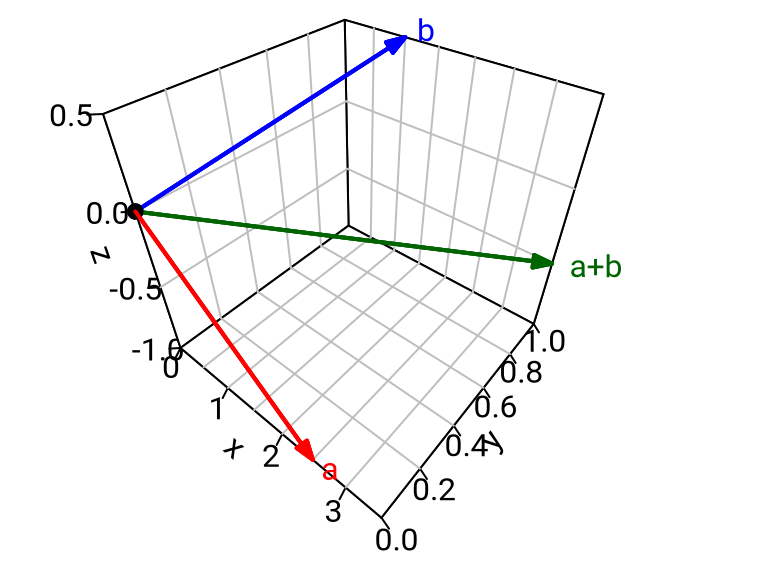
\includegraphics{la2_files/figure-latex/unnamed-chunk-7-1} \end{center}

\begin{enumerate}
\def\labelenumi{(\Roman{enumi})}
\setcounter{enumi}{1}
\item
  \({\color{red}{\underline{a} = (2.5,0,-1)}} \qquad {\color{blue}{\underline{b} = (1,1,0.5)}} \qquad {\color{green}{\underline{a}+\underline{b} = (3.5,1,-0.5)}}\)
\item
  \({\color{red}{\underline{a} = \begin{pmatrix} 1 & 2 & 3 \\ 2.5 & 0 & -1 \end{pmatrix}}} \qquad {\color{blue}{\underline{b} = \begin{pmatrix} 1 & 2 & 3 \\ 1 & 1 & 0.5 \end{pmatrix}}} \qquad {\color{green}{\underline{a}+\underline{b} = \begin{pmatrix} 1 & 2 & 3 \\ 3.5 & 1 & -0.5 \end{pmatrix}}}\)
\item
  \(\begin{aligned} {\color{red}{\underline{a}: \{ 1,2,3}} & {\color{red}{\} \to \mathbb{R}}} & \quad {\color{blue}{\underline{b}: \{ 1,2,3}} & {\color{blue}{\} \to \mathbb{R}}} & \quad {\color{green}{\underline{a}+\underline{b}: \{ 1,2,3}} & {\color{green}{\} \to \mathbb{R}}} \\ & {\color{red}{1 \mapsto 2.5}} & & {\color{blue}{1 \mapsto 1}} & & {\color{green}{1 \mapsto 3.5}} \\ & {\color{red}{2 \mapsto 0}} & & {\color{blue}{2 \mapsto 1}} & & {\color{green}{2 \mapsto 1}} \\ & {\color{red}{3 \mapsto -1}} & & {\color{blue}{3 \mapsto 0.5}} & & {\color{green}{3 \mapsto -0.5}} \end{aligned}\)
\item
\end{enumerate}

\begin{center}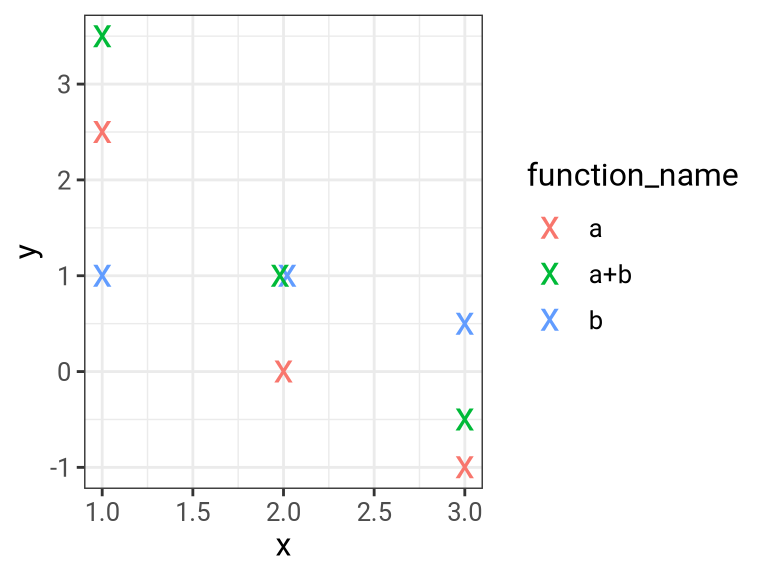
\includegraphics{la2_files/figure-latex/unnamed-chunk-8-1} \end{center}

\csname begin\endcsname{example}\label{cnj:expl-mother}
Let \(S\) be any set and let \(F\) be a field. Let
\[ {\color{red}{F^S}} := \{ f: S \to F \} \]
denote the set of all maps from \(S\) to \(F\).
We define an addition on \(F^{S}\) and a scalar multiplication of \(F\) on \(F^{S}\) as follows:
When \(f,g \in F^{S}\) and \(a \in F\) we set:
\[ \begin{aligned} ({\color{red}{f+g}})(s) & := f(s) + g(s) \qquad & \text{for any } s \in S \\
({\color{red}{af}})(s) & := af(s) & \text{for any } s \in S. \end{aligned} \]
Then \(F^{S}\) is a vector space over \(F\) (see below for the proof).

\emph{Special Cases}:

\begin{enumerate}
\def\labelenumi{(\alph{enumi})}
\item
  Let \(S = \{1,\dots,n\}\). Identifying any map \(f: \{1,\dots,n\} \to F\) with the corresponding tuple \((f(1),\dots,f(n))\), we see that \(F^{S}\) can be identified with the set \(F^{n}\) of all \(n\)-tuples \((a_{1},\dots,a_{n})\) considered in Example \ref{cnj:expl-vectspaces}(a).
\item
  Let \(S = \{1,\dots,n\} \times \{1,\dots,m\}\). Identifying any map \(f: \{1,\dots,n\} \times \{1,\dots,m\} \to F\) with the corresponding matrix: \[ \begin{pmatrix} f((1,1)) & \dots & f((1,m)) \\ \vdots & & \vdots \\ f((n,1)) & \dots & f((n,m)) \end{pmatrix} \] we see that \(F^{S}\) can be identified with the set \(M_{n \times m}(F)\) of \((n \times m)\)-matrices \[ \begin{pmatrix} a_{11} & \dots & a_{1m} \\ \vdots & \ddots & \vdots \\ a_{n1} & \dots & a_{nm} \end{pmatrix} \] with entries in \(F\). In particular \(M_{n \times m}(F)\) is a vector space over \(F\).
\item
  Let \(S = \mathbb{N}\). Identifying any map \(f: \mathbb{N} \to F\) with the sequence \((f(1), f(2), f(3), \dots)\) we see that \(F^{\mathbb{N}}\) can be identified with the set of all infinite sequences \((a_{1},a_{2},a_{3}, \dots)\) in \(F\).
\item
  Let \(F=\mathbb{R}\) and let \(S\) be an interval \(I\) in \(\mathbb{R}\). Then \(F^{S}=\mathbb{R}^I\) is the set of all functions \(f: I \to \mathbb{R}\). (We can visualise these functions via their graph, similarly as in (V) above.)
\end{enumerate}

\csname end\endcsname{example}

\emph{Proof} (that \(F^S\) is a vector space over \(F\)): First, \(F^S\) with the above defined ``\(+\)'' is an abelian group:

\emph{Associativity}: Let \(f,g,h \in F^{S}\).\\
We need to show: \((f+g)+h = f+(g+h) \text{ in } F^{S}\)\\
\hspace*{0.333em}\hspace*{0.333em}\hspace*{0.333em}\hspace*{0.333em}\hspace*{0.333em}\(\iff ((f+g)+h)(s) = (f+(g+h))(s) \qquad\) for all \(s \in S\).\\
\(\left. \begin{aligned} \text{LHS} = (f+g)(s) + h(s) & = (f(s) + g(s)) + h(s) \\  \text{RHS} = f(s) + (g+h)(s) & = f(s) +(g(s) + h(s) \end{aligned} \right\}\) \hfill~{(by definition of addition in \(F^{S}\))}\\
\(\implies\) LHS = RHS \hfill~{(by associativity in \(F\))}

\emph{Identity element}: Let \(\underline{0}\) denote the constant function \(S \to F, s \mapsto 0_{F}\).\\
For any \(f \in F^{S}\) and \(s\in S\) we have \((f + \underline{0})(s) = f(s) + \underline{0}(s) = f(s) + 0_{F} = f(s)\), hence \(f + \underline{0} = f\).\\
Similarly we have \(\underline{0} + f = f\). \hfill~{(using definitions of \(\underline{0}\) and ``\(+\)'', and field axioms)}\\
\(\implies \underline{0}\) is the identity element.

\emph{Inverses}: Let \(f \in F^{S}\). Define \((-f)(s) := -f(s)\).\\
For any \(s\in S\) we have \((f+(-f))(s) = f(s) + (-f)(s) = f(s) + (-f(s)) = 0_F = \underline{0}(s)\).\\
\(\implies f + (-f) = \underline{0}\) in \(F^{S}\), so \(-f\) is the inverse to \(f\). \hfill~{(\(\uparrow\) defns of ``\(+\)'', ``\(-f\)'', \(\underline{0}\), and field axioms)}

\emph{Commutativity}: Let \(f,g\in F^S\).\\
For any \(s\in S\) we have \((f+g)(s)=f(s)+g(s) = g(s) + f(s) = (g+f)(s)\).\\
\(\implies f+g=g+f\). \hfill~{(\(\uparrow\) by the definition of ``\(+\)'', and commutativity of \(+\) in \(F\))}

Now the four axioms from Definition \ref{cnj:defn-vectorspace} (only (i) and (iii) spelled out here, the others are similar):

\emph{First distributivity law}: Let \(a,b \in F\) and \(f \in F^{S}\). We want to check that \((a+b)f = af + bf\):\\
For all \(s \in S\) we have\\
\(((a+b)f)(s) = (a+b)(f(s))\) \hfill~{(by definition of the scalar multiplication)}\\
\hspace*{0.333em}\hspace*{0.333em}\hspace*{0.333em}\hspace*{0.333em} \(= a(f(s)) + b(f(s))\) \hfill~{(by distributivity in \(F\))}\\
\hspace*{0.333em}\hspace*{0.333em}\hspace*{0.333em}\hspace*{0.333em} \(= (af)(s) + (bf)(s)\) \hfill~{(by definition of the scalar multiplication)}\\
\hspace*{0.333em}\hspace*{0.333em}\hspace*{0.333em}\hspace*{0.333em} \(= (af + bf)(s)\) \hfill~{(by definition of addition in \(F^{S}\))}\\
\(\implies (a+b)f = af + bf\).

\emph{Axiom (iii)}: Let \(a,b\in F\) and \(f\in F^S\). We want to check that \((ab)f = a(bf)\).\\
For all \(s\in S\) we have\\
\(((ab)f)(s) = (ab)(f(s))\) \hfill~{(by definition of scalar multiplication in \(F^S\))}\\
\hspace*{0.333em}\hspace*{0.333em}\hspace*{0.333em}\hspace*{0.333em} \(=a(b(f(s)))\) \hfill~{(by associativity of multiplication in \(F\))}\\
\hspace*{0.333em}\hspace*{0.333em}\hspace*{0.333em}\hspace*{0.333em} \(=a((bf)(s))\) \hfill~{(by definition of scalar multiplication in \(F^S\))}\\
\hspace*{0.333em}\hspace*{0.333em}\hspace*{0.333em}\hspace*{0.333em} \(=(a(bf))(s)\) \hfill~{(by definition of scalar multiplication in \(F^S\))}\\
\(\implies\) \((ab)f = a(bf)\). \hfill~{\(\square\)}

\hypertarget{ss-subspaces}{%
\subsection{Subspaces}\label{ss-subspaces}}

\csname begin\endcsname{definition}\label{cnj:defn-subspace}
Let \(V\) be a vector space over a field \(F\). A subset \(W\) of \(V\) is called a \textcolor{red}{subspace of $V$} if the following conditions hold:

\begin{enumerate}
\def\labelenumi{(\alph{enumi})}
\tightlist
\item
  \(0_{V} \in W\).
\item
  \emph{``\(W\) is closed under addition''}: for all \(x,y \in W\) we also have \(x+y \in W\).
\item
  \emph{``\(W\) is closed under scalar multiplication''}: for all \(a \in F\) and \(x \in W\) we have \(ax \in W\).
\end{enumerate}

\csname end\endcsname{definition}

Note that condition (b) states that the restriction of the addition in \(V\) to \(W\) gives a binary operation \(W \times W \to W\) on \(W\) (addition in \(W\)).
Similarly, condition (c) states that the scalar multiplication of \(F\) on \(V\) yields a map \(F \times W \to W\) which we view as a scalar multiplication of \(F\) on \(W\).

\csname begin\endcsname{proposition}\label{cnj:prop-subspace-is-VS}
Let \(V\) be a vector space over a field \(F\) and let \(W\) be a subspace of \(V\).
Then \(W\) together with the above mentioned addition and scalar multiplication is a vector space over \(F\).
\csname end\endcsname{proposition}

\emph{Proof}:
The following axioms hold for \(W\) because they already hold for \(V\):

\begin{itemize}
\tightlist
\item
  associativity of addition;
\item
  commutativity of addition;
\item
  all the four axioms in Definition \ref{cnj:defn-vectorspace}.
\end{itemize}

There exists an additive identity element in \(W\) by condition \ref{cnj:defn-subspace}(a) (i.e.~\(0_W:=0_V\in W\)).\\
It remains to show that additive inverses exist:
Let \(x \in W\). Then \(-x = (-1)x\) (see \ref{cnj:prop-vsbasics}(d)) is in \(W\) by condition \ref{cnj:defn-subspace}(c);
and \(-x\) satisfies \(x+(-x) = 0_W=0_V\) because it does so in \(V\).
\hfill~{\(\square\)}

\csname begin\endcsname{example}\label{cnj:expl-subspaces}

\begin{enumerate}
\def\labelenumi{(\alph{enumi})}
\item
  Examples of subspaces of \(\mathbb{R}^{n}\) as seen in Linear Algebra I, such as the nullspace of any real \((n \times m)\)-matrix, or the column space of any real \((m\times n)\)-matrix.
\item
  The set of convergent sequences is a subspace of the vector space \(\mathbb{R}^{\mathbb{N}}\) of all sequences \((a_{1},a_{2},a_{3}, \dots)\) in \(\mathbb{R}\). A subspace of this subspace (and hence of \(\mathbb{R}^{\mathbb{N}}\)) is the set of all sequences in \(\mathbb{R}\) that converge to \(0\). (See Calculus I for proofs).
\item
  Let \(A \in M_{l \times m}(\mathbb{R})\). Then \(W := \{B \in M_{m \times n}(\mathbb{R}) \mid AB = \underline{0} \}\) is a subspace of \(M_{m \times n}(\mathbb{R})\).\\
  \emph{Proof}:

  \begin{enumerate}
  \def\labelenumii{(\roman{enumii})}
  \tightlist
  \item
    We have \(A \cdot \underline{0} = \underline{0} \implies \underline{0} \in W\).
  \item
    Let \(B_{1},B_{2} \in W\)\\
    \(\implies A(B_{1} + B_{2}) = AB_{1} + AB_{2} = \underline{0} + \underline{0} = \underline{0}\)\\
    \(\implies B_{1} + B_{2} \in W\).
  \item
    Let \(a \in \mathbb{R}\) and \(B \in W\)\\
    \(\implies A(aB) = a(AB) = a \underline{0} = \underline{0}\)\\
    \(\implies aB \in W\). \hfill~{\(\square\)}
  \end{enumerate}
\item
  Let \(I\) be a non-empty interval in \(\mathbb{R}\). The following subsets of the vector space \(\mathbb{R}^{I}\) consisting of all functions from \(I\) to \(\mathbb{R}\) are subspaces:

  \begin{enumerate}
  \def\labelenumii{(\roman{enumii})}
  \tightlist
  \item
    For any \(s_{0} \in I\) the subset \(W := \{ f \in \mathbb{R}^{I} : f(s_{0})=0 \}\) of \(\mathbb{R}^{I}\).\\
    \emph{Proof}:

    \begin{enumerate}
    \def\labelenumiii{(\arabic{enumiii})}
    \tightlist
    \item
      The zero function \(\underline{0}\) vanishes at \(s_{0} \implies \underline{0} \in W\).
    \item
      Let \(f,g \in W\)\\
      \(\implies (f+g)(s_{0}) = f(s_{0}) + g(s_{0}) = 0 + 0 = 0\)\\
      \(\implies f+g \in W\).
    \item
      Let \(a \in \mathbb{R}\) and \(f \in W\)\\
      \(\implies (af)(s_{0}) = a\cdot f(s_{0}) = a\cdot 0 = 0\)\\
      \(\implies af \in W\). \hfill~{\(\square\)}
    \end{enumerate}
  \item
    The set of all continuous functions \(f: I \to \mathbb{R}\) (see Calculus I).
  \item
    The set of all differentiable functions \(f: I \to \mathbb{R}\) (see Calculus I).
  \item
    For any \(n \in \mathbb{N}\), the set \textcolor{red}{$\mathbb{P}_n$} of polynomial functions \(f: I \to \mathbb{R}\) of degree at most \(n\), is a subspace by \ref{cnj:expl-spans}(c) and \ref{cnj:prop-spans}.
    A function \(f: I \to \mathbb{R}\) is a \textcolor{red}{polynomial function of degree at most $n$} if there exists \(a_{0}, \dots ,a_{n} \in \mathbb{R}\) such that:
    \[ f(s) = a_{0} + a_{1}s + \dots + a_{n}s^{n} \text{ for all } s \in I. \]
    Denoting the function \(I \to \mathbb{R}, s \mapsto s^{m}\), by \textcolor{red}{$t^m$}, this means that \(f = a_{0}t^0 + a_{1}t^1 + \dots + a_{n}t^{n}\) as elements of the vector space \(\mathbb{R}^{I}\).
    (We will also use the more natural notation \(1\) for \(t^0\), and \(t\) for \(t^1\).)
  \item
    The space of solutions of a homogeneous linear differential equation (without further explanation); e.g.: \[ \mathbb{P}_{n} = \{ f \in \mathbb{R}^{I} : f \text{ is differentiable } (n+1) \text{ times and } f^{(n+1)} = \underline{0} \} \]
  \end{enumerate}
\item
  The subset \(\mathbb{Z}^{n}\) of the vector space \(\mathbb{R}^{n}\) over \(\mathbb{R}\) is closed under addition but not closed under scalar multiplication: For instance, \((1,0, \dots ,0) \in \mathbb{Z}^{n}\) and \(\frac{1}{2} \in \mathbb{R}\), but \(\frac{1}{2}(1,0, \dots ,0) \notin \mathbb{Z}^{n}\).
\item
  The subsets \(W_{1} := \{ (a,0) : a \in \mathbb{R} \}\) and \(W_{2} := \{ (0,b) : b \in \mathbb{R} \}\) are subspaces of \(\mathbb{R}^{2}\). The subset \(W := W_{1} \cup W_{2}\) of the vector space \(\mathbb{R}^{2}\) is closed under scalar multiplication but not under addition because, for instance, \((1,0)\) and \((0,1)\) are in \(W\) but \((1,0) + (0,1) = (1,1) \notin W\).
\end{enumerate}

\csname end\endcsname{example}

\csname begin\endcsname{proposition}\label{cnj:prop-sum-int-subspaces}
Let \(W_{1},W_{2}\) be subspaces of a vector space \(V\) over a field \(F\).
Then the intersection \(W_{1} \cap W_{2}\) and the \textcolor{red}{sum of subspaces}
\[ {\color{red}{W_{1} + W_{2}}} := \{ x_{1} + x_{2}\in V \mid x_{1} \in W_{1}, \ x_{2} \in W_{2} \} \]
are subspaces of \(V\) as well.
\csname end\endcsname{proposition}

\emph{Proof}: \emph{For \(W_{1} \cap W_{2}\)}:

\begin{enumerate}
\def\labelenumi{(\alph{enumi})}
\tightlist
\item
  We have \(0_V\in W_1\) and \(0_V\in W_2\) \hfill~{(because \(W_1\) and \(W_2\) are subspaces)}\\
  \(\implies\) \(0_V\in W_1\cap W_2\). \hfill~{(by definition of intersection)}
\item
  Let \(x,y\in W_1\cap W_2\)\\
  \(\implies\) \(x,y \in W_1\) and \(x,y\in W_2\) \hfill~{(by definition of intersection)}\\
  \(\implies\) \(x+y\in W_1\) and \(x+y\in W_2\) \hfill~{(because \(W_1\) and \(W_2\) are subspaces)}\\
  \(\implies\) \(x+y\in W_1\cap W_2\). \hfill~{(by definition of intersection)}
\item
  Let \(a\in F\) and \(x\in W_1\cap W_2\)\\
  \(\implies\) \(x \in W_1\) and \(x\in W_2\) \hfill~{(by definition of intersection)}\\
  \(\implies\) \(ax\in W_1\) and \(ax\in W_2\) \hfill~{(because \(W_1\) and \(W_2\) are subspaces)}\\
  \(\implies\) \(ax\in W_1\cap W_2\). \hfill~{(by definition of intersection)}
\end{enumerate}

\emph{For \(W_{1} + W_{2}\)}:

\begin{enumerate}
\def\labelenumi{(\alph{enumi})}
\tightlist
\item
  We have \(0_{V} = 0_{V} + 0_{V} \in W_{1} + W_{2}\).
\item
  Let \(x,y \in W_{1} + W_{2}\)\\
  \(\implies \exists x_{1},y_{1} \in W_{1}\) and \(\exists x_{2},y_{2} \in W_{2}\) with \(x=x_{1}+x_{2}\), \(y=y_{1}+y_{2}\)
  \hfill~{(by definition of \(W_1+W_2\))}\\
  \(\implies x + y = (x_{1}+x_{2}) + (y_{1}+y_{2}) =\)\\
  \hspace*{0.333em}\hspace*{0.333em}\hspace*{0.333em}\hspace*{0.333em}\hspace*{0.333em}\hspace*{0.333em}\(=(x_{1}+y_{1}) + (x_{2}+y_{2}) \in W_{1} + W_{2}\).
  \hfill~{(because \(W_{1}\) and \(W_{2}\) are subspaces)}
\item
  Let \(a \in F\) and \(x \in W_{1} + W_{2}\)\\
  \(\implies \exists x_{1} \in W_{1}\), \(x_{2} \in W_{2}\) such that \(x=x_{1}+x_{2}\) \hfill~{(by definition of \(W_1+W_2\))}\\
  \(\implies ax = a (x_{1}+x_{2}) = ax_{1} + ax_{2} \in W_{1} + W_{2}\).
  \hfill~{(because \(W_{1}\) and \(W_{2}\) are subspaces)\quad\(\square\)}
\end{enumerate}

\csname begin\endcsname{example}\label{cnj:expl-subspace-sumofaxes}
Let \(W_{1}\) and \(W_{2}\) be as in \ref{cnj:expl-subspaces}(f). Then \(W_{1} + W_{2} = \mathbb{R}^{2}\).
\csname end\endcsname{example}

\newpage

\hypertarget{bases}{%
\section{Bases}\label{bases}}

\hypertarget{ss-spanning}{%
\subsection{Spanning}\label{ss-spanning}}

\csname begin\endcsname{definition}\label{cnj:defn-span}
Let \(V\) be a vector space over a field \(F\).
Let \(x_1, \dots, x_n \in V\).

\begin{enumerate}
\def\labelenumi{(\alph{enumi})}
\tightlist
\item
  An element \(x \in V\) is called a \textcolor{red}{linear combination of $x_1, \dots, x_n$} if there are \(a_1, \dots, a_n \in F\) such that \(x = a_1x_1 + \dots + a_nx_n\).
\item
  The subset of \(V\) consisting of all linear combinations of \(x_1, \dots, x_n\) is called the \textcolor{red}{span of $x_1, \dots, x_n$} and is denoted by \textcolor{red}{$\mathrm{Span}(x_1, \dots, x_n)$} (or \textcolor{red}{$\mathrm{Span}_F(x_1, \dots, x_n)$}); i.e.
  \[ \mathrm{Span}(x_1, \dots, x_n) = \{ a_1x_1 + \dots + a_nx_n \mid a_1, \dots,  a_n \in F \}. \]
\item
  We say that \(x_1, \dots, x_n\) \textcolor{red}{span} \(V\), or that \(x_1, \dots x_n\) \textcolor{red}{form a spanning set of $V$}, if \(V = \mathrm{Span}(x_1, \dots, x_n)\), i.e.~every \(x \in V\) is a linear combination of \(x_1, \dots, x_n\).
\end{enumerate}

\textcolor{green}{(See also Section 6.3 of L.A.I.)}
\csname end\endcsname{definition}

\csname begin\endcsname{example}\label{cnj:expl-spans}

\begin{enumerate}
\def\labelenumi{(\alph{enumi})}
\item
  Let \(V := M_{n \times m}(F)\) be the vector space of \((n \times m)\)-matrices with entries in \(F\). For \(i \in \{1, \dots, n \}\) and \(j \in \{1, \dots, m\}\), let \(E_{ij}\) denote the \((n \times m)\)-matrix with zeroes everywhere except at \((ij)\) where it has the entry \(1\). Then the matrices \(E_{ij}; i=1, \dots, n ; j=1, \dots, m\) form a spanning set of \(V\).\\
  \emph{Proof}: Let \(A = (a_{ij}) \in M_{n \times m}(F)\) be an arbitrary matrix. Then \(A = \sum_{i=1}^n \sum_{j=1}^m a_{ij} E_{ij}\).\\
  For example: \(\left(\begin{smallmatrix} 2 & 3 \\ -1 & 5 \end{smallmatrix}\right) = 2 \left(\begin{smallmatrix} 1 & 0 \\ 0 & 0 \end{smallmatrix}\right) + 3 \left(\begin{smallmatrix} 0 & 1 \\ 0 & 0 \end{smallmatrix}\right) + (-1) \left(\begin{smallmatrix} 0 & 0 \\ 1 & 0 \end{smallmatrix}\right) + 5 \left(\begin{smallmatrix} 0 & 0 \\ 0 & 1 \end{smallmatrix}\right)\) \(= 2E_{11}+3E_{12}+(-1)E_{21}+5E_{22}.\)
\item
  Do the vectors \(\begin{pmatrix} 1 \\ i \end{pmatrix}, \begin{pmatrix} i \\ 2 \end{pmatrix} \in \mathbb{C}^2\) span the vector space \(\mathbb{C}^2\) over \(\mathbb{C}\)?\\
  \emph{Solution}: Let \(\begin{pmatrix} w \\ z \end{pmatrix} \in \mathbb{C}^2\) be an arbitrary vector.\\
  We want to know if we can find \(a_1, a_2 \in \mathbb{C}\) such that \(a_1 \begin{pmatrix} 1 \\ i \end{pmatrix} + a_2 \begin{pmatrix} i \\ 2 \end{pmatrix} = \begin{pmatrix} w \\ z \end{pmatrix}\).\\
  Hence \(\left( \begin{array}{ c c | c } 1 & i & w \\ i & 2 & z \end{array} \right) \xrightarrow{R2 \mapsto R2 - iR1} \left( \begin{array}{ c c | c } 1 & i & w \\ 0 & 3 & z-iw \end{array} \right)\).\\
  As in Linear Algebra I we conclude that this system is solvable. \textcolor{green}{(Theorem 3.15 of L.A.I.)}\\
  Thus \(\begin{pmatrix} 1 \\ i \end{pmatrix}, \begin{pmatrix} i \\ 2 \end{pmatrix}\) span \(\mathbb{C}^2\).
\item
  \(\mathbb{P}_n = \mathrm{Span}(t^0,t^1,t^2, \dots, t^n) = \mathrm{Span}(1,t,t^2, \dots, t^n)\) (c.f. \ref{cnj:expl-subspaces}(d)(iv)).
\end{enumerate}

\csname end\endcsname{example}

\csname begin\endcsname{proposition}\label{cnj:prop-spans}
Let \(V\) be a vector space over a field \(F\).
Let \(x_1, \dots, x_n \in V\).
Then \(\mathrm{Span}(x_1, \dots, x_n)\) is the smallest subspace of \(V\) that contains \(x_1, \dots, x_n\).
Furthermore:

\begin{enumerate}
\def\labelenumi{(\alph{enumi})}
\item
  If \(x \in \mathrm{Span}(x_1, \dots ,x_n)\) then \(\mathrm{Span}(x_1, \dots, x_n,x) = \mathrm{Span}(x_1, \dots, x_n)\).
\item
  For any \(a_2, \dots, a_n \in F\) we have \(\mathrm{Span}(x_1, \dots, x_n) = \mathrm{Span}(x_1, x_2-a_2x_1, \dots, x_n- a_nx_1)\).
\end{enumerate}

\csname end\endcsname{proposition}

\emph{Notes}:

\begin{itemize}
\item
  The first statement means:

  \begin{enumerate}
  \def\labelenumi{\arabic{enumi}.}
  \tightlist
  \item
    \(\mathrm{Span}(x_1, \dots, x_n)\) is a subspace of \(V\) that contains \(x_1, \dots, x_n\), \emph{and}
  \item
    among all the subspaces of \(V\) with this property it is the smallest;\\
    in other words if \(W\) is a subspace of \(V\) that contains \(x_1, \dots, x_n\), then \(\mathrm{Span}(x_1, \dots x_n) \subseteq W\).
  \end{enumerate}
\item
  The statement (b) implies that the span of the column vectors of any matrix does not change when performing (standard) column operations.
\end{itemize}

\emph{Proof}: \emph{\(\mathrm{Span}(x_1, \dots, x_n)\) is a subspace of \(V\)}:

\begin{enumerate}
\def\labelenumi{(\roman{enumi})}
\tightlist
\item
  We have \(0_{V} = 0_{F}x_1 + \dots + 0_{F}x_n \in \mathrm{Span}(x_1, \dots, x_n)\).
\item
  Let \(x,y \in \mathrm{Span}(x_1, \dots, x_n)\).\\
  \(\implies \exists a_1, \dots, a_n \in F, \ \exists b_1, \dots b_n \in F\) such that
  ~~~~\(x= a_1x_1 + \dots + a_nx_n\) and \(y = b_1x_1 + \dots + b_nx_n\);\\
  \(\implies x+y = (a_1x_1 + \dots + a_nx_n) + (b_1x_1 + \dots + b_nx_n)\)\\
  \hspace*{0.333em}\hspace*{0.333em}\hspace*{0.333em}\hspace*{0.333em}\(= (a_1x_1 + b_1x_1) + \dots + (a_nx_n + b_nx_n)\) \hfill~{(using commutativity and associativity)}\\
  \hspace*{0.333em}\hspace*{0.333em}\hspace*{0.333em}\hspace*{0.333em}\(= (a_1 + b_1)x_1 + \dots + (a_n + b_n)x_n\) \hfill~{(using first distributivity law)}\\
  \hspace*{0.333em}\hspace*{0.333em}\hspace*{0.333em}\hspace*{0.333em}\(\in \mathrm{Span}(x_1, \dots, x_n)\) \hfill~{(by definition of Span)}
\item
  Let \(x \in \mathrm{Span}(x_1, \dots, x_n)\) and \(a \in F\).\\
  Write \(x= a_1x_1 + \dots a_nx_n\) with \(a_1, \dots, a_n \in F\) as above.\\
  \(\implies ax = a(a_1x_1 + \dots + a_nx_n)\)
  ~~~~\(= a(a_1x_1) + \dots + a(a_nx_n)\) \hfill~{(using distributivity)}\\
  \hspace*{0.333em}\hspace*{0.333em}\hspace*{0.333em}\hspace*{0.333em}\(= (a a_1)x_1 + \dots + (a a_n)x_n\) \hfill~{(by axiom \ref{cnj:defn-vectorspace}(iii))}\\
  \hspace*{0.333em}\hspace*{0.333em}\hspace*{0.333em}\hspace*{0.333em}\(\in \mathrm{Span}(x_1, \dots, x_n)\) \hfill~{(by definition of Span)}
\end{enumerate}

\emph{\(\mathrm{Span}(x_1, \dots, x_n)\) contains \(x_1, \dots, x_n\)}:\\
\hspace*{0.333em}\hspace*{0.333em}\hspace*{0.333em}\hspace*{0.333em}\ldots{} because \(x_{i} = 0_{F}\cdot x_1 + \dots 0_{F}\cdot x_{i-1} + 1 \cdot x_{i} + 0_{F}\cdot x_{i+1} + \dots + 0_{F}\cdot x_n\) \(\in \mathrm{Span}(x_1,\dots,x_n)\).

\emph{\(\mathrm{Span}(x_1, \dots, x_n\)) is the smallest}:\\
\hspace*{0.333em}\hspace*{0.333em}\hspace*{0.333em}\hspace*{0.333em} Let \(W\) be a subspace of \(V\) such that \(x_1, \dots, x_n \in W\).\\
\hspace*{0.333em}\hspace*{0.333em}\hspace*{0.333em}\hspace*{0.333em} Let \(x \in \mathrm{Span}(x_1, \dots, x_n)\). Write \(x = a_1x_1 + \dots + a_nx_n\) with \(a_1, \dots a_n \in F\).\\
\hspace*{0.333em}\hspace*{0.333em}\hspace*{0.333em}\hspace*{0.333em} \(\implies\) \(a_1x_1, \dots, a_nx_n \in W\) \hfill~{(by condition \ref{cnj:defn-subspace}(c))}\\
\hspace*{0.333em}\hspace*{0.333em}\hspace*{0.333em}\hspace*{0.333em} \(\implies\) \(x = a_1x_1 + \dots + a_nx_n \in W\). \hfill~{(by condition \ref{cnj:defn-subspace}(b))}\\
\hspace*{0.333em}\hspace*{0.333em}\hspace*{0.333em}\hspace*{0.333em} \(\implies\) \(\mathrm{Span}(x_1,\dots,x_n)\subseteq W\).

\emph{Part (a)}: \(\mathrm{Span}(x_1, \dots, x_n) \subseteq \mathrm{Span}(x_1, \dots, x_n,x) =: W\)\\
\hspace*{0.333em}\hfill~{(because \(W\) is a subspace of \(V\) and \(x_1, \dots, x_n \in W\))}\\
\hspace*{0.333em}\hspace*{0.333em}\hspace*{0.333em}\hspace*{0.333em} \(\mathrm{Span}(x_1, \dots, x_n,x) \subseteq \mathrm{Span}(x_1, \dots, x_n) =: \widetilde{W}\)\\
\hspace*{0.333em}\hfill~{(because \(\widetilde{W}\) is a subspace of \(V\) and \(x_1, \dots, x_n,x \in \widetilde{W}\))}

\emph{Part (b)}: \(\mathrm{Span}(x_1, \dots, x_n) \subseteq \mathrm{Span}(x_1, x_2-a_2x_1, \dots, x_n-a_nx_1) =: W\)\\
\hspace*{0.333em}\hfill~{(because \(W\) is a subspace of \(V\) and \(x_1, \dots, x_n \in W\))}\\
\hspace*{0.333em}\hspace*{0.333em}\hspace*{0.333em}\hspace*{0.333em} \(\mathrm{Span}(x_1, x_2-a_2x_1, \dots, x_n-a_nx_1) \subseteq \mathrm{Span}(x_1, \dots, x_n) =: \widetilde{W}\)\\
\hspace*{0.333em}\hfill~{(because \(\widetilde{W}\) is a subspace of \(V\) and \(x_1\in \widetilde{W}\) and for \(i=2,\dots,n\) also \(x_i-a_ix_1 \in \widetilde{W}\))\(\square\)}

\hypertarget{ss-lin-indep}{%
\subsection{Linear independence}\label{ss-lin-indep}}

\csname begin\endcsname{definition}\label{cnj:defn-lin-indep}
Let \(V\) be a vector space over a field \(F\).
Let \(x_1, \dots, x_n \in V\).
We say that \(x_1, \dots, x_n\) are \textcolor{red}{linearly independent (over $F$)} if the following condition holds:

~~~~if \(a_1, \dots, a_n \in F\) and \(a_1x_1 + \dots + a_nx_n = 0_V\) ~~~~ then ~~~~ \(a_1 = \dots = a_n = 0_F\).

Otherwise we say that \(x_1, \dots, x_n\) are \textcolor{red}{linearly dependent}.
A linear combination \(a_1x_1+\dots+a_nx_n\) is called \textcolor{red}{trivial} if \(a_1=\dots=a_n=0\), otherwise it is called \textcolor{red}{non-trivial}.
\textcolor{green}{(See also Section 6.5 of L.A.I.)}

\csname end\endcsname{definition}

\emph{Note}:
\(x_1,\dots,x_n\) are linearly dependent \(\iff\) \(\exists a_1,\dots,a_n\in F\), not all zero, such that \(a_1x_1+\dots+a_nx_n=0_V\).
In other words, \(\iff\) there exists a non-trivial linear combination of \(x_1,\dots,x_n\) which equals \(0_V\).

\csname begin\endcsname{example}\label{cnj:expl-lin-indep}

\begin{enumerate}
\def\labelenumi{(\alph{enumi})}
\item
  Examples as seen in Linear Algebra I. \textcolor{green}{(Section 6.5 of L.A.I.)}
\item
  The three vectors \(\underline{x}_1 = \begin{pmatrix} 1 \\ 0 \\ 1 \end{pmatrix}\),
  \(\underline{x}_2 = \begin{pmatrix} 1 \\ 1 \\ 0 \end{pmatrix}\),
  \(\underline{x}_3 = \begin{pmatrix} 0 \\ -1 \\ 1 \end{pmatrix} \in F^3\)
  are \emph{not} linearly independent because \(\underline{x}_1 - \underline{x}_2 - \underline{x}_3 = \underline{0}\).
\item
  Determine all vectors \(\begin{pmatrix} c_1 \\ c_2 \\ c_3 \end{pmatrix} \in \mathbb{C}^3\)
  such that \(\underline{x}_1:= \begin{pmatrix} 1 \\ i \\ 1 \end{pmatrix}\),
  \(\underline{x}_2:= \begin{pmatrix} 0 \\ 1 \\ 0 \end{pmatrix}\),
  \(\underline{x}_3:= \begin{pmatrix} c_1 \\ c_2 \\ c_3 \end{pmatrix} \in \mathbb{C}^3\) are linearly dependent.\\
  \emph{Solution}: We apply Gaussian elimination:
  \[\begin{pmatrix} 1 & 0 & c_1 \\ i & 1 & c_2 \\ 1 & 0 & c_3 \end{pmatrix}
  \xrightarrow[R2 \mapsto R2 - iR1]{R3 \mapsto R3 - R1}
  \begin{pmatrix} 1 & 0 & c_1 \\ 0 & 1 & c_2 - ic_1 \\ 0 & 0 & c_3 - c_1 \end{pmatrix}\]\\
  \hspace*{0.333em}\hspace*{0.333em}\hspace*{0.333em}\hspace*{0.333em}\(\implies\) The equation \(a_1\underline{x}_1 + a_2\underline{x}_2 + a_3\underline{x}_3 = \underline{0}\) has a non-trivial solution \((a_1, a_2, a_3)\)\\
  \hspace*{0.333em}\hspace*{0.333em}\hspace*{0.333em}\hspace*{0.333em} ~~~~ ~~~~ ~~~~ if and only if \(c_3 - c_1 = 0\).\\
  \hspace*{0.333em}\hspace*{0.333em}\hspace*{0.333em}\hspace*{0.333em}\(\implies\) \(\underline{x}_1, \underline{x}_2, \underline{x}_3\) are linearly dependent if and only if \(c_1 = c_3\).
\item
  The two functions \(\sin , \cos \in \mathbb{R}^{\mathbb{R}}\) are linearly independent.\\
  \emph{Proof}: Let \(a,b \in \mathbb{R}\) such that \(a \sin + b \cos = \underline{0}\) in \(\mathbb{R}^{\mathbb{R}}\).\\
  \hspace*{0.333em}\hspace*{0.333em}\hspace*{0.333em}\hspace*{0.333em} \(\implies\) For all \(s\in \mathbb{R}\) we have \(a\cdot\sin(s) + b\cdot \cos(s) = \underline{0}(s) = 0\).\\
  \hspace*{0.333em}\hspace*{0.333em}\hspace*{0.333em}\hspace*{0.333em} \(\implies \begin{cases} a\cdot \sin (0) + b\cdot \cos (0) = 0 \implies a \cdot 0 + b \cdot 1 = 0 \implies b=0 \\ a\cdot \sin (\frac{\pi}2) + b\cdot \cos (\frac{\pi}2) = 0 \implies a \cdot 1 + b \cdot 0 = 0 \implies a=0 \end{cases}\) \hfill~{\(\square\)}
\item
  Let \(I \subseteq \mathbb{R}\) be a non-empty open interval.
  Recall from \ref{cnj:expl-subspaces}(d)(iv) that for any \(i \in \mathbb{N}_{0}\),
  we denote \(t^{i}\) the polynomial function
  \(I \rightarrow \mathbb{R}, s \mapsto s^{i}\).\\
  The vectors \(t^0,t^1,t^2, \dots, t^n\) are linearly independent in \(\mathbb{R}^{I}\).\\
  \emph{Proof}: Let \(a_{0}, \dots, a_n \in \mathbb{R}\) such that \(a_{0}t^0 + a_1t^1 + \dots + a_nt^n = \underline{0}\)\\
  \hspace*{0.333em}\hspace*{0.333em}\hspace*{0.333em}\hspace*{0.333em} \(\implies a_{0} + a_1s + \dots + a_ns^n = 0\) for all \(s \in I\)\\
  \hspace*{0.333em}\hspace*{0.333em}\hspace*{0.333em}\hspace*{0.333em} \(\implies a_{0} = \dots = a_n = 0\), because any non-zero real polynomial of degree \(n\) has at most \(n\) real roots. (This follows from the Fundamental Theorem of Algebra. Alternatively, it can be proved by induction and using long division.)
\end{enumerate}

\csname end\endcsname{example}

\csname begin\endcsname{proposition}\label{cnj:prop-lin-indep-basics}
Let \(V\) be a vector space over a field \(F\).

\begin{enumerate}
\def\labelenumi{(\alph{enumi})}
\item
  A single vector \(x \in V\) is linearly independent if and only if \(x \neq 0_{V}\).
\item
  Every subset of any set of linearly independent vectors is linearly independent again.
  (This is equivalent to: If a subset of a set of vectors is linearly dependent, then the set
  itself is linearly dependent.)
\item
  Let \(x_1, \dots, x_n \in V\) and suppose that \(x_{i} = 0_{V}\) for some \(i \in \{1, \dots, n \}\),
  or that \(x_{i} = x_{j}\) for some \(i \neq j\). Then \(x_1, \dots, x_n\) are linearly dependent.
\item
  If \(x_1, \dots, x_n \in V\) are linearly dependent then at least one vector \(x_{i}\)
  among \(x_1, \dots, x_n\) is a linear combination of the other ones.
\item
  Let \(x_1, \dots, x_n \in V\) and \(x \in \mathrm{Span}(x_1, \dots, x_n)\).
  Then \(x_1, \dots, x_n, x\) are linearly dependent.
\end{enumerate}

\csname end\endcsname{proposition}

\emph{Proof}:

\begin{enumerate}
\def\labelenumi{(\alph{enumi})}
\item
  ``\(\Rightarrow\)'': If \(x=0_{V}\) then \(1 \cdot x = 0_{V}\) is a non-trivial linear combination of \(x\).\\
  ``\(\Leftarrow\)'': Let \(x \neq 0_{V}\) and let \(a \in F\) such that \(ax = 0_{V}\). Then \(a=0\) by \ref{cnj:prop-vsbasics}(c).
\item
  Let \(x_1, \dots, x_n \in V\) be linearly independent and let \(y_1, \dots, y_m\) be a subset of \(x_1, \dots, x_n\) for some \(m \leq n\).\\
  Proceed by contradiction: Suppose that \(\exists b_1, \dots, b_m \in F\), not all zero,
  such that \(b_1y_1 + \dots + b_my_m = 0_{V}\).\\
  Extending the list \(b_1, \dots, b_m\) by zeroes we get \(a_1, \dots, a_n \in F\), not all zero,
  such that \(a_1x_1 + \dots + a_nx_n = 0_{V}\).\\
  So \(x_1, \dots, x_n\) are linearly dependent, a contradiction.
\item
  If \(x_{i} = 0_{V}\) then \(x_1, \dots, x_n\) are linearly dependent by (a) and (b).\\
  If \(x_{i} = x_{j}\) for some \(i \neq j\), then \(x_{i}, x_{j}\) are linearly dependent, because \(1x_{i} + (-1)x_{j} = 0_{V}\). Now apply (b).
\item
  \(\exists a_1, \dots, a_n \in F\), not all zero, such that \(a_1x_1 + \dots + a_nx_n = 0_{V}\).\\
  After reordering we may assume \(a_n \neq 0\).\\
  \(\implies x_n = -a_n^{-1} (a_1x_1 + \dots + a_nx_n)\) \(= (-a_n^{-1} a_1)x_1 + \dots + (-a_n^{-1} a_{n-1})x_{n-1}\)\\
  \(\implies\) \(x_n\) is a linear combination of \(x_1, \dots, x_{n-1}\).
\item
  Let \(x\in\mathrm{Span}(x_1,\dots,x_n)\).\\
  \(\implies\) \(\exists a_1, \dots, a_n \in F\), such that \(x = a_1x_1 + \dots + a_nx_n\).\\
  \(\implies 0_{V} = a_1x_1 + \dots + a_nx_n + (-1)x\)\\
  \(\implies\) We have a a non-trivial linear combination of \(x_1, \dots, x_n,x\) which equals \(0_V\).\\
  \hspace*{0.333em}\hfill~{(Because \(-1\not=0\) in any field.) \(\square\)}
\end{enumerate}

\hypertarget{ss-bases}{%
\subsection{Bases}\label{ss-bases}}

\csname begin\endcsname{definition}\label{cnj:defn-basis}
Let \(V\) be a vector space over a field \(F\).
Let \(x_1, \dots, x_n \in V\).
We say that \(x_1, \dots, x_n\) \textcolor{red}{form a basis of $V$}
if \(x_1, \dots, x_n\) both span \(V\) and are linearly independent.
\textcolor{green}{(Compare Definition 6.40 of L.A.I.)}
\csname end\endcsname{definition}

\csname begin\endcsname{example}\label{cnj:expl-bases}

\begin{enumerate}
\def\labelenumi{(\alph{enumi})}
\item
  Let \(F\) be a field. The vectors \textcolor{red}{$\underline{e}_1$} \(:= (1,0, \dots, 0)\); \ldots{} ; \textcolor{red}{$\underline{e}_n$} \(:= (0, \dots, 0,1)\) form a basis \(F^n\), called the \textcolor{red}{standard basis of $F^n$} (as in Linear Algebra I \textcolor{green}{(Ex 6.41(a)}).
\item
  The polynomials \(1,t, \dots, t^n\) form a basis of \(\mathbb{P}_n\). (see \ref{cnj:expl-subspaces}(d)(iv), \ref{cnj:expl-spans}(c)).
\item
  \(1,i\) form a basis of the vector space \(\mathbb{C}\) over \(\mathbb{R}\) (cf \ref{cnj:expl-vectspaces}(b)).
\item
  Determine a basis of the nullspace \(N(A) \subseteq \mathbb{R}^4\) of the matrix
  \[ A := \begin{pmatrix} 1 & -1 & 3 & 2 \\ 2 & -1 & 6 & 7 \\ 3 & -2 & 9 & 9 \\ -2 & 0 & -6 & -10 \end{pmatrix} \in M_{4 \times 4}(\mathbb{R}).\]\\
  \emph{Solution}: We perform Gaussian elimination until the reduced lower echelon form (row operations):
  \begin{align*} A = \begin{pmatrix} 1 & -1 & 3 & 2 \\ 2 & -1 & 6 & 7 \\ 3 & -2 & 9 & 9 \\ -2 & 0 & -6 & -10 \end{pmatrix}
  &\xrightarrow[\substack{R3 \mapsto R3 - 3R1 \\ R4 \mapsto R4 + 2R1}]{R2 \mapsto R2 - 2R1}
  \begin{pmatrix} 1 & -1 & 3 & 2 \\ 0 & 1 & 0 & 3 \\ 0 & 1 & 0 & 3 \\ 0 & -2 & 0 & -6 \end{pmatrix}
  \\
  &\xrightarrow[\substack{R3 \mapsto R3 - R2 \\ R4 \mapsto R4 + 2R2}]{R1 \mapsto R1 + R2}
  \begin{pmatrix} 1 & 0 & 3 & 5 \\ 0 & 1 & 0 & 3 \\ 0 & 0 & 0 & 0 \\ 0 & 0 & 0 & 0 \end{pmatrix} =: \widetilde{A}
  \end{align*}
  Because performing row operations does not change the nullspace of a matrix (see Note below), we have:
  \begin{align*}
  N(A) &= N(\widetilde{A}) = \{ \underline{x} \in \mathbb{R}^4 : \widetilde{A} \underline{x} = \underline{0} \}
  \\ & = \left\{ \begin{pmatrix} x_1 \\ x_2 \\ x_3 \\ x_4 \end{pmatrix} \in \mathbb{R}^4 : x_1 = -3x_3 - 5x_4 ; \ x_2 = -3x_4 \right\}
  \\ & = \left\{ \begin{pmatrix} -3x_3 - 5x_4 \\ -3x_4 \\ x_3 \\ x_4 \end{pmatrix} : x_3, x_4 \in \mathbb{R} \right\}
  \\ & = \left\{ x_3 \begin{pmatrix} -3 \\ 0 \\ 1 \\ 0 \end{pmatrix} + x_4 \begin{pmatrix} -5 \\ -3 \\ 0 \\ 1 \end{pmatrix} : x_3, x_4 \in \mathbb{R} \right\}
  \\ & = \mathrm{Span}\left( \begin{pmatrix} -3 \\ 0 \\ 1 \\ 0 \end{pmatrix}, \begin{pmatrix} -5 \\ -3 \\ 0 \\ 1 \end{pmatrix} \right).
  \end{align*}
  (Denote \(\underline{u}_1=(-3,0,1,0)^T\), \(\underline{u}_2=(-5,-3,0,1)^T\)).\\
  \(\bullet\) \(\underline{u}_1\) and \(\underline{u}_2\) are also linearly independent (because they are not multiples of each other).\\
  \(\implies\) \(\underline{u}_1\) and \(\underline{u}_2\) form a basis of \(N(A)\).
\end{enumerate}

\begin{enumerate}
\def\labelenumi{(\alph{enumi})}
\setcounter{enumi}{4}
\tightlist
\item
  Let \(A \in M_{n \times n}(\mathbb{R})\). Then:\\
  \(A\) invertible \(\iff\) The columns of \(A\) form a basis of \(\mathbb{R}^n\) (for a proof see Theorem \ref{cnj:thm-detiff}).
\end{enumerate}

\csname end\endcsname{example}

\emph{Note}: Row operations do not change the nullspace of a matrix (say \(A\)).
This is because vectors \(\underline{x}\) are in \(N(A)\) exactly if they are solutions to \(A\underline{x}=\underline{0}\),
i.e.~solutions to the homogeneous system of linear equations described by the matrix \(A\).
Row operations on \(A\) correspond to the ``allowed'' operations on the linear system of equations.

\csname begin\endcsname{proposition}\label{cnj:prop-basisiff}
Let \(V\) be a vector space over a field \(F\).
Let \(x_1, \dots, x_n \in V\). The following statements are equivalent:

\begin{enumerate}
\def\labelenumi{(\alph{enumi})}
\tightlist
\item
  \(x_1, \dots, x_n\) form a basis of \(V\).
\item
  \(x_1, \dots, x_n\) form a \textcolor{red}{minimal spanning set of $V$} (i.e.~\(x_1, \dots, x_n\) span \(V\) and after removing any vector from \(x_1, \dots, x_n\) the remaining ones don't span \(V\) anymore). \textcolor{green}{(Compare Def 6.23 of L.A.I.)}
\item
  \(x_1, \dots, x_n\) form a \textcolor{red}{maximal linearly independent subset of $V$} (i.e.~\(x_1, \dots, x_n\) are linearly independent and for any \(x \in V\) the \(n+1\) vectors \(x_1, \dots, x_n,x\) are linearly dependent).
\item
  Every vector \(x \in V\) can be written in the form \[ x = a_1x_1 + \dots + a_nx_n \] with coefficients \(a_1, \dots, a_n \in F\) uniquely determined by x.
\end{enumerate}

\csname end\endcsname{proposition}

\emph{Proof}:
``\emph{(a) \(\implies\) (b)}'': 1/\emph{Spanning}: \(x_1, \dots, x_n\) span \(V\) by definition of a basis.\\
2/\emph{Minimality}: Suppose that the spanning set \(x_1, \dots, x_n\) is not minimal.\\
\(\implies\) After reordering we may assume that \(x_1, \dots, x_{n-1}\) span \(V\).\\
\(\implies x_n \in V = \mathrm{Span}(x_1, \dots, x_{n-1})\).\\
\(\implies x_1, \dots, x_{n-1},x_n\) are linearly dependent (by \ref{cnj:prop-lin-indep-basics}(e)). Contradiction.

\emph{(b) \(\implies\) (c)}: 1/\emph{Independence}: Suppose that \(x_1, \dots, x_n\) are linearly dependent.\\
\(\implies\) After reordering we have \(x_n \in \mathrm{Span}(x_1, \dots, x_{n-1})\) (by \ref{cnj:prop-lin-indep-basics}(d))\\
\(\implies\) \(V = \mathrm{Span}(x_1, \dots, x_n) = \mathrm{Span}(x_1, \dots, x_{n-1})\) (by \ref{cnj:prop-spans}(a))\\
This contradicts the minimality assumed in (b).\\
2/\emph{Maximality}: Let \(x \in V = \mathrm{Span}(x_1, \dots, x_n)\)\\
\(\implies x_1, \dots, x_n, x\) are linearly dependent (by \ref{cnj:prop-lin-indep-basics}(c)).

\emph{(c) \(\implies\) (d)}: 1/\emph{Existence}: Let \(x \in V\).\\
\(\implies \exists b_1, \dots, b_n, b \in F\), not all zero, with \(b_1x_1 + \dots + b_nx_n + bx = 0\).\\
\hspace*{0.333em}\hfill~{(because \(x_1, \dots, x_n,x\) are linearly dependent)}\\
\(\implies b \neq 0\) \hfill~{(because \(x_1, \dots, x_n\) are linearly independent)}\\
\(\implies x = a_1x_1 + \dots + a_nx_n\), where \(a_{i} := -b^{-1}b_{i}\).\\
2/\emph{Uniqueness}: Suppose \(x = a_1x_1 + \dots + a_nx_n = b_1x_1 + \dots + b_nx_n\) for some \(a_1,\dots,a_n,b_1,\dots,b_n\in F\).\\
\(\implies 0_{V} = x-x = (a_1 - b_1)x_1 + \dots + (a_n - b_n)x_n\)\\
\(\implies a_1 = b_1, \dots, a_n=b_n\). \hfill~{(because \(x_1, \dots, x_n\) are linearly independent)}

\emph{(d) \(\implies\) (a)}: 1/\emph{Spanning}: Directly from (d).\\
2/\emph{Independence}: Let \(a_1, \dots, a_n \in F\) such that \(a_1x_1 + \dots a_nx_n = 0_{V}\).\\
\(\implies a_1 = \dots = a_n = 0\). \hfill~{(from uniqueness, because also \(0x_1 + \dots + 0x_n = 0_{V}\)) \(\square\)}

\csname begin\endcsname{corollary}\label{cnj:coro-basis-exists}
Let \(V\) be a vector space over a field \(F\).
Suppose \(V = \mathrm{Span}(x_1, \dots, x_n)\) for some \(x_1, \dots x_n \in V\).
Then a subset of \(x_1, \dots, x_n\) forms a basis of \(V\). In particular \(V\) has a basis.
\csname end\endcsname{corollary}

\emph{Proof}:
By successively removing vectors from \(x_1, \dots, x_n\) we arrive at a minimal spanning set \(y_1, \dots, y_m\)
for some \(m \leq n\). Then \(y_1, \dots, y_m\) form a basis of \(V\) (by \ref{cnj:prop-basisiff} (b) \(\implies\) (a)).
\hfill~{\(\square\)}

\hypertarget{ss-dimension}{%
\subsection{Dimension}\label{ss-dimension}}

\csname begin\endcsname{theorem}\label{cnj:thm-vsdim}
\textcolor{blue}{(This Theorem allows us to define the dimension of a vector space.)}\\
Let \(V\) be a vector space over a field \(F\).
Suppose \(x_1, \dots, x_n\) and \(y_1, \dots, y_m\) both form a basis of \(V\). Then \(m = n\).
\textcolor{green}{(Compare Thm 6.44 from L.A.I.)}
\csname end\endcsname{theorem}

\csname begin\endcsname{definition}\label{cnj:defn-vsdim}
Let \(V\) be a vector space over a field \(F\).
If the vectors \(x_1, \dots, x_n \in V\) form a basis of \(V\), we say that \textcolor{red}{$V$ is of finite dimension},
and call \(n\) the \textcolor{red}{dimension of $V$}. We write \textcolor{red}{$\mathrm{dim}_{F}(V)$}
or just \textcolor{red}{$\mathrm{dim}(V)$} for \(n\).
Note that \(n\) does not depend on the chosen basis \(x_1, \dots, x_n\) by \ref{cnj:thm-vsdim}.
\csname end\endcsname{definition}

\csname begin\endcsname{example}\label{cnj:expl-vsdim1}

\begin{enumerate}
\def\labelenumi{(\alph{enumi})}
\tightlist
\item
  \(\mathrm{dim}_{F}(F^n)=n\) ~~ (by Example \ref{cnj:expl-bases}(a)).
\item
  \(\mathrm{dim}_{\mathbb{R}}(\mathbb{P}_n) = n + 1\) ~~ (by Example \ref{cnj:expl-bases}(b)).
\item
  \(\mathrm{dim}_{\mathbb{R}}(\mathbb{C}) = 2\) ~~ (by Example \ref{cnj:expl-bases}(c)).
\item
  \(\mathrm{dim}_{\mathbb{C}}(\mathbb{C}^3) = 3\), \(\mathrm{dim}_{\mathbb{R}}(\mathbb{C}^3) = 6\). In general
  \(\mathrm{dim}_{\mathbb{C}}(\mathbb{C}^n) = n\), \(\mathrm{dim}_{\mathbb{R}}(\mathbb{C}^n) = 2n\).
\item
  \(\mathbb{R}\) as a vector space over \(\mathbb{Q}\) is \emph{not} finite dimensional (see \ref{cnj:expl-vectspaces}(b)).
\item
  \(\mathrm{dim}_{\mathbb{R}}(M_{n \times m}(\mathbb{R})) = nm\).
\item
  \(\mathrm{dim}_{\mathbb{Q}}(\mathbb{Q}(\sqrt{-3})) = 2\) (see Coursework 2).
\item
  About \(\mathrm{dim}_F(\mathrm{Span}(x_1,\dots,x_n))\).
  We determine its dimension by finding a basis, i.e.~subset of \(x_1,\dots,x_n\) which still spans
  \(\mathrm{Span}(x_1,\dots,x_n)\), and it is linearly independent. For example:\\
  Let \(x_1 \in V, \ x_1 \neq 0 \implies \mathrm{dim}_{F}(\mathrm{Span}(x_1)) = 1\).\\
  Let \(x_2\) be another vector in \(V\).\\
  \(\implies \mathrm{dim}_{F}(\mathrm{Span}(x_1,x_2)) = \begin{cases} 2 & \text{if } x_1,x_2 \text{ are linearly independent} \\ 1 & \text{if } x_1,x_2 \text{ are linearly dependent} \end{cases}\)
\end{enumerate}

\csname end\endcsname{example}

\emph{Proof of Theorem \ref{cnj:thm-vsdim}}:
It follows from the following Proposition.
\hfill~{\(\square\)}

\csname begin\endcsname{proposition}\label{cnj:prop-vsdim-proof}
Let \(V\) be a vector space over a field \(F\). Let \(x_1, \dots, x_n \in V\) and \(y_1, \dots, y_m \in V\).\\
Suppose \(x_1, \dots, x_n\) span \(V\). If \(y_1, \dots, y_m\) are linearly independent then \(m \leq n\).
\csname end\endcsname{proposition}

\emph{Proof}:
We will show the contrapositive:

\begin{itemize}
\tightlist
\item
  If \(m > n\) then there exist \(c_1, \dots, c_m \in F\), not all zero, such that \(c_1y_1 + \dots + c_my_m = 0\).
\end{itemize}

For every \(i \in \{1, \dots, m\}\) we can write \(y_{i} = a_{i1}x_1+ \dots +a_{in}x_n\) for some \(a_{i1}, \dots a_{in} \in F\).\\
\hspace*{0.333em}\hfill~{(because \(x_1, \dots, x_n\) span \(V\))}\\
\(\implies\) For all \(c_1, \dots, c_m \in F\) we have: \hfill~{(using the axioms of a vector space)}
\begin{align*}
c_1y_1 + \dots + c_my_m &= c_1(a_{11}x_1 + \dots + a_{1n}x_n) + \dots + c_{m}(a_{m1}x_1 + \dots + a_{mn}x_n)
\\ &= (a_{11}c_1 + \dots + a_{m1}c_m)x_1 + \dots + (a_{1n}c_1 + \dots + a_{mn}c_m)x_n
\end{align*}
\(\implies\) It suffices to show that the system of linear equations
\begin{align*}
a_{11}c_1 + a_{21}c_2 + \dots + a_{m1}c_m &= 0\\
&\vdots\\
a_{1n}c_1 + a_{2n}c_2 + \dots + a_{mn}c_m &= 0
\end{align*}
has a solution \((c_1, \dots, c_m) \in F^m\) different from \((0, \dots, 0)\).\\
This follows from Gaussian elimination (as seen in Linear Algebra I for \(F=\mathbb{R}\) \textcolor{green}{(Thm 3.15(b) from L.A.I.)}):
since \(m>n\), we have more unknowns than equations.
\hfill~{\(\square\)}

\csname begin\endcsname{corollary}\label{cnj:coro-two-out-of-three}
\textcolor{blue}{(Two-out-of-three basis criterion.)}\\
Let \(V\) be a vector space over a field \(F\).
Let \(x_1, \dots x_n \in V\). Suppose two of the following three statements hold.
Then \(x_1, \dots, x_n\) form a basis:

\begin{enumerate}
\def\labelenumi{(\alph{enumi})}
\tightlist
\item
  \(x_1, \dots, x_n\) are linearly independent.
\item
  \(x_1, \dots, x_n\) span \(V\).
\item
  \(n = \mathrm{dim}_{F}(V)\).
\end{enumerate}

\csname end\endcsname{corollary}

\emph{Proof}:
If (a) and (b) hold, then \(x_1, \dots, x_n\) form a basis by definition.\\
Suppose (a) and (c) hold. If \(x_1, \dots, x_n\) would not form a basis we could find an \(x \in V\) such that \(x_1, \dots, x_n,x\) are still linearly independent (by \ref{cnj:prop-basisiff} (a) \(\iff\) (c)).\\
\(\implies\) \(n+1 \leq n\) by Proposition \ref{cnj:prop-vsdim-proof}. Contradiction.\\
Suppose (b) and (c) hold. After reordering we may assume that \(x_1, \dots, x_m\) form a minimal spanning set, for some \(m \leq n\).\\
\(\implies x_1, \dots, x_m\) form a basis (by \ref{cnj:prop-basisiff} (a) \(\iff\) (b)).\\
\(\implies m=n\) (by \ref{cnj:thm-vsdim}); i.e.~\(x_1, \dots, x_n\) form a basis.
\hfill~{\(\square\)}

\csname begin\endcsname{example}\label{cnj:expl-vsdim2}

\begin{enumerate}
\def\labelenumi{(\alph{enumi})}
\item
  The vectors \(\underline{x}_1:= \begin{pmatrix} 1 \\ 2 \\ 3 \end{pmatrix}\),
  \(\underline{x}_2:= \begin{pmatrix} -2 \\ 1 \\ 0 \end{pmatrix}\),
  \(\underline{x}_3:= \begin{pmatrix} 1 \\ 0 \\ 1 \end{pmatrix}\)
  form a basis of the vector space \(\mathbb{Q}^3\) over \(\mathbb{Q}\),
  of the vector space \(\mathbb{R}^3\) over \(\mathbb{R}\)
  and of the vector space \(\mathbb{C}^3\) over \(\mathbb{C}\).\\
  \hspace*{0.333em}\\
  \emph{Proof}:
  We first show that \(\underline{x}_1, \underline{x}_2, \underline{x}_3\) are linearly independent over \(\mathbb{C}\):\\
  Let \(c_1, c_2, c_3 \in \mathbb{C}\) such that \(c_1 \underline{x}_1 + c_2 \underline{x}_2 + c_3 \underline{x}_3 =0\).
  \[
  \implies \quad \begin{pmatrix} 1 & -2 & 1 \\ 2 & 1 & 0 \\ 3 & 0 & 1 \end{pmatrix} \begin{pmatrix} c_1 \\ c_2 \\ c_3 \end{pmatrix} = \begin{pmatrix} 0 \\ 0 \\ 0 \end{pmatrix}.
  \]
  Gaussian elimination yields:
  \[
  A:= \begin{pmatrix} 1 & -2 & 1 \\ 2 & 1 & 0 \\ 3 & 0 & 1 \end{pmatrix}
  \xrightarrow[R3 \mapsto R3 - 3R1]{R2 \mapsto R2 - 2R1}
  \begin{pmatrix} 1 & -2 & 1 \\ 0 & 5 & -2 \\ 0 & 6 & -2 \end{pmatrix}
  \xrightarrow{R3 \mapsto R3 - \frac{6}5 R2}
  \begin{pmatrix} 1 & -2 & 1 \\ 0 & 5 & -2 \\ 0 & 0 & 2/5 \end{pmatrix}
  \]
  \(\implies\) \(\underline{c}= (c_1,c_2,c_3) = (0,0,0)\) is the only solution of \(A \underline{c} = 0\).\\
  \(\implies\) \(\underline{x}_1, \underline{x}_2, \underline{x}_3\) are linearly independent over \(\mathbb{C}\) and then also over \(\mathbb{R}\) and \(\mathbb{Q}\).\\
  \(\implies\) \(\underline{x}_1, \underline{x}_2, \underline{x}_3\) form a basis of \(\mathbb{C}^3\), \(\mathbb{R}^3\) and \(\mathbb{Q}^3\) over the respective fields.\\
  \hspace*{0.333em}\hfill~{(by \ref{cnj:coro-two-out-of-three} since \(3 = \mathrm{dim}_{\mathbb{C}}(\mathbb{C}^3) = \mathrm{dim}_{\mathbb{R}}(\mathbb{R}^3) = \mathrm{dim}_{\mathbb{Q}}(\mathbb{Q}^3)\)) \(\square\)}
\item
  We view \(\mathbb{C}\) as a vector space over \(\mathbb{C}\), \(\mathbb{R}\) and \(\mathbb{Q}\) (see \ref{cnj:expl-vectspaces}(b)).\\
  Let \(x_1:=1, x_2:=2, x_3:=\sqrt2, x_4:=i, x_5:=i\sqrt3 \in \mathbb{C}\).\\
  Determine \(\mathrm{dim}_{F}(\mathrm{Span}_{F}(x_1,x_2,x_3,x_4,x_5))\) for \(F = \mathbb{C}\), \(\mathbb{R}\) and \(\mathbb{Q}\).\\
  \hspace*{0.333em}\\
  \emph{Solution}: \emph{For \(F=\mathbb{C}\)}:\\
  We have \(\mathbb{C} = \mathrm{Span}_{\mathbb{C}}(x_1) \subseteq \mathrm{Span}_{\mathbb{C}}(x_1, \dots, x_5) \subseteq \mathbb{C}\).\\
  \(\implies\) \(\mathrm{dim}_{\mathbb{C}}(\mathrm{Span}_{\mathbb{C}}(x_1, \dots, x_5))\)
  \(= \mathrm{dim}_{\mathbb{C}}(\mathbb{C}) = 1\).\\
  \hspace*{0.333em}\\
  \emph{For \(F=\mathbb{R}\)}:\\
  \(x_1\) and \(x_4\) span \(\mathbb{C}\) as a vector space over \(\mathbb{R}\).\\
  \(\implies\) \(\mathrm{Span}_{\mathbb{R}}(x_1, \dots, x_5) = \mathbb{C}\).\\
  \(\implies\) \(\mathrm{dim}_{\mathbb{R}}(\mathrm{Span}(x_1, \dots, x_5))\)
  \(= \mathrm{dim}_{\mathbb{R}}(\mathbb{C}) = 2\).\\
  \hspace*{0.333em}\\
  \emph{For \(F=\mathbb{Q}\)}: Observations:\\
  \(x_1,x_2\) are LD over \(\mathbb{Q}\) \(\implies\) \(\mathrm{Span}_\mathbb{Q}(x_1,\dots,x_5) = \mathrm{Span}_\mathbb{Q}(x_1,x_3,x_4,x_5)\).\\
  Also \(x_1,x_3\) are LI over \(\mathbb{Q}\); \(x_1,x_4\) are LI over \(\mathbb{R}\).\\
  \(\leadsto\) Let us try to prove that \(x_1,x_3,x_4,x_5\) are linearly independent over \(\mathbb{Q}\).\\
  Let \(a_1,a_3,a_4,a_5\in\mathbb{Q}\) be such that \(a_1x_1+a_3x_3+a_4x_4+a_5x_5=0\).\\
  \(\implies\) \((a_1 + a_3\sqrt2) + i(a_4 + a_5\sqrt3) = 0\).\\
  \(\implies\) \(a_1+a_3\sqrt{2}=0\) and \(a_4+a_5\sqrt3=0\)
  \hfill~{(because \(1\) and \(i\) are linearly independent over \(\mathbb{Q}\))}\\
  \(\implies\) \(a_1=a_3=0\)
  \hfill~{(If \(a_3\not=0\) \(\implies\) \(\sqrt{2}=-\frac{a_1}{a_3}\in\mathbb{Q}\). Contradiction.)}\\
  \hspace*{0.333em}\hspace*{0.333em}\hspace*{0.333em}\hspace*{0.333em}\hspace*{0.333em} and \(a_4=a_5=0\) (similarly).\\
  \(\implies\) \(x_1, x_3,x_4,x_5\) are linearly independent, so form a basis of \(\mathrm{Span}_\mathbb{Q}(x_1,x_3,x_4,x_5)\).\\
  \(\implies\) \(\mathrm{dim}_\mathbb{Q}(\mathrm{Span}_\mathbb{Q}(x_1,x_2,x_3,x_4,x_5)) =\)
  \(\mathrm{dim}_\mathbb{Q}(\mathrm{Span}_\mathbb{Q}(x_1,x_3,x_4,x_5)) = 4\).
\item
  Let \(V\) be a vector space of finite dimension over a field \(F\) and let \(W\) be a subspace of \(V\).
  Then \(\mathrm{dim}_{F}(W) \leq \dim_F(V)\).\\
  \hspace*{0.333em}\\
  \emph{Proof}: If vectors are L.I. in \(W\), they are also L.I. in \(V\). \hfill~{(by def. of L.I.)}\\
  \(\implies\) Any L.I. subset of \(W\) has at most \(\mathrm{dim}(V)\) elements \hfill~{(use \ref{cnj:prop-vsdim-proof} and \ref{cnj:prop-basisiff}(a)\(\iff\)(c))}\\
  \(\implies\) \(\mathrm{dim}(W)\leq\mathrm{dim}(V)\) \hfill~{(by \ref{cnj:prop-basisiff}(a)\(\iff\)(c))}
\end{enumerate}

\csname end\endcsname{example}

\newpage

\hypertarget{lt}{%
\section{Linear Transformations}\label{lt}}

Let \(F\) be a field (e.g.~\(F = \mathbb{R}, \mathbb{Q}, \mathbb{C}\) or \(\mathbb{F}_{2}\)).

\csname begin\endcsname{definition}\label{cnj:defn-matrix}
An \textcolor{red}{$m \times n$-matrix $A$ over a field $F$} is an array
\[ A = \begin{pmatrix} a_{11} & \dots & a_{1n} \\ \vdots & & \vdots \\ a_{m1} & \dots & a_{mn} \end{pmatrix} \]
with entries \(a_{ij}\) in \(F\).
We use the notation \textcolor{red}{$M_{m \times n}(F)$} for the set of all \((m \times n)\)-matrices over \(F\) (see also \ref{cnj:expl-mother}(b)).
We define \textcolor{red}{addition and multiplication of matrices} (and other notions) in the same way as in the case \(F = \mathbb{R}\) (as seen in Linear Algebra I).
\csname end\endcsname{definition}

For example:

\begin{itemize}
\tightlist
\item
  \(\begin{pmatrix} 1 & 1+i \\ 2 & 1-i \end{pmatrix} \begin{pmatrix} 1-i \\ 3 \end{pmatrix} = \begin{pmatrix} 1-i + 3+3i \\ 2-2i + 3-3i \end{pmatrix} = \begin{pmatrix} 4+2i \\ 5-5i \end{pmatrix}\) ~~ (matrices over \(\mathbb{C}\))
\item
  \(\begin{pmatrix} 0 & 1 \\ 1 & 1 \end{pmatrix} \begin{pmatrix} 1 & 1 \\ 0 & 1 \end{pmatrix} = \begin{pmatrix} 0 & 1 \\ 1 & 0 \end{pmatrix}\) ~~ (as matrices over \(\mathbb{F}_{2}\))
\item
  but \(\begin{pmatrix} 0 & 1 \\ 1 & 1 \end{pmatrix} \begin{pmatrix} 1 & 1 \\ 0 & 1 \end{pmatrix} = \begin{pmatrix} 0 & 1 \\ 1 & 2 \end{pmatrix}\) ~~ (as matrices over \(\mathbb{R}\))
\end{itemize}

\csname begin\endcsname{definition}\label{cnj:defn-lt}
Let \(V, W\) be vector spaces over a field \(F\).
A map \(L: V \to W\) is called a \textcolor{red}{linear transformation} if the following two conditions hold:

\begin{enumerate}
\def\labelenumi{(\alph{enumi})}
\tightlist
\item
  For all \(x,y \in V\) we have \(L(x + y) = L(x) + L(y)\) in \(W\).
\item
  For all \(a \in F\) and \(x \in V\) we have \(L(ax) = a(L(x))\) in \(W\).
\end{enumerate}

\csname end\endcsname{definition}

\emph{Note}: Then we also have \(L( 0_{V}) = 0_{W}\) and \(L(x-y) = L(x) - L(y)\) for all \(x,y \in V\).

\emph{Proof}: \(L(0_{V}) = L(0_{V} + 0_{V}) = L(0_{V}) + L(0_{V})\)\\
\(\implies\) \(L(0_{V}) = 0_{W}\). \hfill~{(by cancelling \(L(0_{V})\))}\\
\(L(x-y) = L(x+(-1)y) = L(x) + L((-1)y) = L(x) + (-1)L(y) = L(x) - L(y)\).
\hfill~{(using \ref{cnj:prop-vsbasics}(d)) \(\square\)}

\csname begin\endcsname{example}\label{cnj:expl-lt}

\begin{enumerate}
\def\labelenumi{(\alph{enumi})}
\item
  Let \(A \in M_{m \times n}(F)\). Then the map
  \begin{align*} {\color{red}{L_{A}}}: &F^{n} \to F^{m} \\
  &\underline{x} = \begin{pmatrix} x_{1} \\ \vdots \\ x_{n} \end{pmatrix} \mapsto
  A \underline{x} = \begin{pmatrix} a_{11}x_{1} + \dots + a_{1n}x_{n} \\ \vdots \\ a_{m1}x_{1} + \dots + a_{mn}x_{n} \end{pmatrix}
  \end{align*}
  is a linear transformation. \textcolor{green}{(Compare with Lemma 5.3 in L.A.I.)}\\
  For example, if \(A = \begin{pmatrix} a & 0 \\ 0 & a \end{pmatrix} \in M_{2 \times 2}(\mathbb{R})\) for some \(a \in \mathbb{R}\) then \(L_{A} : \mathbb{R}^{2} \to \mathbb{R}^{2}\) is given by \(\underline{x} \mapsto a \underline{x}\), i.e.~it is a stretch of the plane by a factor of a.\\
  If \(A = \begin{pmatrix} \cos(\phi) & \sin(\phi) \\ -\sin(\phi) & \cos(\phi) \end{pmatrix}\) for some \(0 \leq \phi < 2\pi\) then \(L_{A}: \mathbb{R}^{2} \to \mathbb{R}^{2}\) is the clockwise rotation by the angle \(\phi\).\\
  \hspace*{0.333em}\\
  \emph{Proof that \(L_A\) is a linear transformation}:\\
  1/ Let \(\underline{x},\underline{y} \in F^{n}\).\\
  \hspace*{0.333em}\hspace*{0.333em}\hspace*{0.333em}\(\implies\) \(L_{A}( \underline{x}+\underline{y}) = A(\underline{x}+\underline{y}) = A \underline{x} + A \underline{y} = L_{A}(\underline{x}) + L_{A}(\underline{y})\).\\
  2/ Let \(a \in F\) and \(\underline{x} \in F^{n}\).\\
  \hspace*{0.333em}\hspace*{0.333em}\hspace*{0.333em}\(\implies\) \(L_{A}(a \underline{x}) = A(a \underline{x}) = a (A \underline{x}) = a(L_{A}(\underline{x}))\).\\
  (The middle equality of both chains of equalities has been proved in Linear Algebra I for \(F= \mathbb{R}\), \textcolor{green}{see Thm 2.13(i) and (ii)}, the same proof works for any field \(F\).)
  \hfill~{\(\square\)}
\item
  Let \(V\) be a vector space over a field \(F\). Then the following maps are linear transformations (cf.~\textcolor{green}{Example 5.4(c),(d) in L.A.I.}):

  \begin{itemize}
  \tightlist
  \item
    \textcolor{red}{id}\(: V \to V\), \(x \mapsto x\) ~~ (\textcolor{red}{identity})
  \item
    \textcolor{red}{$\underline{0}$}\(:V \to V\), \(x \mapsto 0_{V}\) ~~ (\textcolor{red}{zero map})
  \item
    the map \(V \to V\), given by \(x \mapsto ax\), for any given \(a\in F\) fixed (stretch)
  \end{itemize}
\item
  Let \(L: V \to W\) and \(M: W \to Z\) be linear transformation between vector spaces over a field \(F\).
  Then their composition \(M \circ L: V \to Z\) is again a linear transformation. \textcolor{green}{(See also Section 5.3 of L.A.I.)}\\
  \hspace*{0.333em}\\
  \emph{Proof that \(M\circ L\) is a linear transformation}:\\
  1/ Let \(x,y \in V\).\\
  \hspace*{0.333em}\hspace*{0.333em}\hspace*{0.333em}\(\implies\) \((M \circ L)(x+y) =\) \(M(L(x+y)) =\) \(M(L(x) + L(y))\)\\
  \hspace*{0.333em}\hspace*{0.333em}\hspace*{0.333em}\hspace*{0.333em}\hspace*{0.333em}\hspace*{0.333em}\hspace*{0.333em}\hspace*{0.333em}\hspace*{0.333em}\hspace*{0.333em}\(= M(L(x)) + M(L(y)) =\) \((M \circ L)(x) + (M \circ L)(y)\).\\
  2/ Let \(a\in F\) and \(x \in V\).\\
  \hspace*{0.333em}\hspace*{0.333em}\hspace*{0.333em}\(\implies\) \((M \circ L)(ax) =\) \(M(L(ax)) =\) \(M(a(L(x))) =\) \(a(M(L(x))) =\) \(a(M \circ L)(x)\).
  \hfill~{\(\square\)}
\item
  Let \(V\) be the subspace of \(\mathbb{R}^{\mathbb{R}}\) consisting of all differentiable functions.
  Then differentiation \(D: V \to \mathbb{R}^{\mathbb{R}}\), \(f \mapsto f'\), is a linear transformation.\\
  \hspace*{0.333em}\\
  \emph{Proof}:\\
  1/ Let \(f,g \in V\) \(\implies\) \(D(f+g) = (f+g)' = f' + g' = D(f) + D(g)\).\\
  2/ Let \(a \in \mathbb{R}\) and \(f \in V\) \(\implies\) \(D(af) = (af)' = a f' = a(D(f))\).\\
  (The middle equality in both chains of equalities has been proved in Calculus.)
  \hfill~{\(\square\)}
\item
  The map \(L: \mathbb{R}^{2} \to \mathbb{R}\), \(\begin{pmatrix} x_{1} \\ x_{2} \end{pmatrix} \mapsto x_{1}x_{2}\), is not a linear transformation.\\
  \emph{Proof}: Let \(a=2\) and \(\underline{x} = \begin{pmatrix} 1 \\ 1 \end{pmatrix} \in \mathbb{R}^{2}.\) Then:\\
  \(L(a \underline{x}) = L \Bigg( \begin{pmatrix} 2 \\ 2 \end{pmatrix} \Bigg) = 4\), but \(aL( \underline{x}) = 2 \cdot 1 = 2\).
  \hfill~{\(\square\)}
\end{enumerate}

\csname end\endcsname{example}

\hypertarget{ss-matrep-1}{%
\subsection{Matrix representation I}\label{ss-matrep-1}}

\csname begin\endcsname{proposition}\label{cnj:prop-matrep-1}
\textcolor{blue}{(Matrix representation I)}\\
Let \(F\) be a field.
Let \(L: F^{n} \to F^{m}\) be a linear transformation. Then there exists a unique matrix \(A \in M_{m \times n}(F)\) such that \(L = L_{A}\) (as defined in \ref{cnj:expl-lt}(a)). In this case we say that \textcolor{red}{$A$ represents $L$ (with respect to the standard bases of $F^{n}$ and $F^{m}$)}.

\textcolor{green}{(See also Theorem 5.6 of L.A.I.)}
\csname end\endcsname{proposition}

For example, the map \(\mathbb{R}^{3} \to \mathbb{R}^{2}, \begin{pmatrix} c_{1} \\ c_{2} \\ c_{3} \end{pmatrix} \mapsto \begin{pmatrix} 2c_{1} + c_{3} - 4c_{2} \\ c_{2} \end{pmatrix}\), is represented by \(A = \begin{pmatrix} 2 & -4 & 1 \\ 0 & 1 & 0 \end{pmatrix} \in M_{2 \times 3}( \mathbb{R})\).

\emph{Proof}:
Let \(\underline{e}_{1}:= \begin{pmatrix} 1 \\ 0 \\ \vdots \\ 0 \end{pmatrix} , \dots, \underline{e}_{n} := \begin{pmatrix} 0 \\ \vdots \\ 0 \\ 1 \end{pmatrix}\) denote the standard basis of \(F^{n}\).

\emph{Uniqueness}: Suppose \(A \in M_{m \times n}(F) \text{ satisfies } L=L_{A}\).\\
\(\implies\) The \(j^{th}\) column of \(A\) is \(A \underline{e}_{j} = L_{A}( \underline{e}_{j}) = L( \underline{e}_{j}) \ \ (\text{for } j=1, \dots, n)\)\\
\(\implies\) \fbox{$A$ is the $(m \times n)$-matrix with the column vector $L( \underline{e}_{1}), \dots,  L( \underline{e}_{n})$.}

\emph{Existence}: Let \(A\) be defined this way. We want to show \(L = L_{A}\).\\
Let \(\underline{c} = \begin{pmatrix} c_{1} \\ \vdots \\ c_{n} \end{pmatrix} \in F^{n} \implies \underline{c} = c_{1} \underline{e}_{1} + \dots + c_{n} \underline{e}_{n};\)\\
\(\implies L( \underline{c}) = L(c_{1} \underline{e}_{1}) + \dots + L(c_{n} \underline{e}_{n}) = c_{1}L( \underline{e}_{1}) + \dots + c_{n}L( \underline{e}_{n})\)\\
\hspace*{0.333em}\hspace*{0.333em}\hspace*{0.333em}\hspace*{0.333em}and \(L_{A}( \underline{c}) = \phantom{L(c_{1} \underline{e}_{1}) +} \dots \phantom{L(c_{1} \underline{e}_{1}) +} = c_{1}L_{A}( \underline{e}_{1}) + \dots + c_{n}L_{A}( \underline{e}_{n})\)\\
\hspace*{0.333em}\hfill~{(because \(L\) and \(L_{A}\) are linear transformations)}\\
\(\implies\) \(L( \underline{c}) = L_{A}( \underline{c})\) because \(L( \underline{e}_{j}) = L_{A}( \underline{e}_{j})\) for all \(j = 1, \dots, n\)).
\hfill~{\(\square\)}

\hypertarget{ss-kernel-and-image}{%
\subsection{Kernel and image}\label{ss-kernel-and-image}}

\csname begin\endcsname{definition}\label{cnj:defn-ker-im}
Let \(L: V \to W\) be a linear transformation between vector spaces \(V,W\) over a field \(F\). Then
\[ {\color{red}{\mathrm{ker}(L)}} := \{ x \in V : \ L(x)= 0_{W} \} \]
is called the \textcolor{red}{kernel of $L$}, and
\[ {\color{red}{\mathrm{im}(L)}}:= \{ y \in W : \ \exists x \in V : \ y = L(x) \} \]
is called the \textcolor{red}{image of $L$}.
\csname end\endcsname{definition}

\csname begin\endcsname{remark}\label{cnj:rmrk-ker-im-matrix}
Let \(F\) be a field and \(A \in M_{m \times n}(F)\). Then
\[ \mathrm{ker}(L_{A}) = \mathrm{N}(A) \]
where \textcolor{red}{$\mathrm{N}(A)$} \(= \{ \underline{c} \in F^{n} : A \underline{c} = \underline{0} \}\) denotes the \textcolor{red}{nullspace of $A$} \textcolor{green}{(see also Section 6.2 of L.A.I.)} and
\[ \mathrm{im}(L_{A}) = \mathrm{Col}(A) \]
where \(\mathrm{Col}(A)\) denotes the \textcolor{red}{column space of $A$}; i.e.~\textcolor{red}{$\mathrm{Col}(A)$} \(= \mathrm{Span}(\underline{a}_{1}, \dots, \underline{a}_{n})\), where \(\underline{a}_{1}, \dots, \underline{a}_{n}\) denote the \(n\) columns of \(A\). \textcolor{green}{(See also Section 6.4 of L.A.I.)}
\csname end\endcsname{remark}

\emph{Proof}:\\
\emph{First assertion}: by definition.\\
\emph{Second assertion}: follows from \ref{cnj:prop-LT-span-LI}(a) applied to the standard basis of \(F^{n}\).
\hfill~{\(\square\)}

\csname begin\endcsname{proposition}\label{cnj:prop-im-ker-subspaces}
Let \(V\) and \(W\) be vector spaces over a field \(F\) and let \(L: V \to W\) be a linear transformation. Then:

\begin{enumerate}
\def\labelenumi{(\alph{enumi})}
\tightlist
\item
  \(\mathrm{ker}(L)\) is a subspace of \(V\).
\item
  \(\mathrm{im}(L)\) is a subspace of \(W\).
\end{enumerate}

\csname end\endcsname{proposition}

\emph{Proof}: (a) We verify the three subspace axioms.

\begin{enumerate}
\def\labelenumi{(\roman{enumi})}
\tightlist
\item
  We have \(0_{V} \in \mathrm{ker}(L)\) (see Note after Defn \ref{cnj:defn-lt}.)
\item
  Let \(x,y \in \mathrm{ker}(L)\);\\
  \(\implies L(x+y) = L(x) + L(y) = 0_{W} + 0_{W} = 0_{W}\);\\
  \(\implies x+y \in \mathrm{ker}(L)\).
\item
  Let \(a \in F\) and \(x \in \mathrm{ker}(L)\);\\
  \(\implies L(ax) = a(L(x)) = a 0_{W} = 0_{W}\);\\
  \(\implies ax \in \mathrm{ker}(L)\).
\end{enumerate}

(b) We verify the three subspace axioms.

\begin{enumerate}
\def\labelenumi{(\roman{enumi})}
\tightlist
\item
  We have \(0_{W} = L(0_{V}) \in \mathrm{im}(L)\).
\item
  Let \(x,y \in \mathrm{im}(L)\);\\
  \(\implies \exists v,w \in V\) such that \(x=L(v)\) and \(y=L(w)\);\\
  \(\implies x+y = L(v) + L(w) = L(v+w) \in \mathrm{im}(L)\).
\item
  Let \(y \in \mathrm{im}(L)\) and \(a \in F\);\\
  \(\implies \exists x \in V\) such that \(y = L(x)\);\\
  \(\implies ay = a(L(x)) = L(ax) \in \mathrm{im}(L)\).
  \hfill~{\(\square\)}
\end{enumerate}

\csname begin\endcsname{example}\label{cnj:expl-basis-im}
Let \(A \in M_{4 \times 4}(\mathbb{R})\) be as in \ref{cnj:expl-bases}(d). Find a basis of the image, \(\mathrm{im}(L_{A})\), of \(L_{A} : \mathbb{R}^{4} \to \mathbb{R}^{4}, \underline{c} \mapsto A \underline{c}\).
\csname end\endcsname{example}

\emph{Solution}: We perform column operations:
\begin{align*}
A =
\begin{pmatrix} 1 & -1 & 3 & 2 \\ 2 & -1 & 6 & 7 \\ 3 & -2 & 9 & 9 \\ -2 & 0 & -6 & -10 \end{pmatrix}
& \xrightarrow[\substack{C3 \mapsto C3 - 3C1 \\ C4 \mapsto C4 - 2C1}]{C4 \mapsto C4 + 3C2}
\begin{pmatrix} 1 & 0 & 0 & 0 \\ 2 & 1 & 0 & 3 \\ 3 & 1 & 0 & 3 \\ -2 & -2 & 0 & -6 \end{pmatrix}
\\
& \xrightarrow{C2 \mapsto C2 + C1}
\begin{pmatrix} 1 & 0 & 0 & 0 \\ 2 & 1 & 0 & 0 \\ 3 & 1 & 0 & 0 \\ -2 & -2 & 0 & 0 \end{pmatrix} =: \widetilde{A}
\end{align*}\\
\(\implies\) The two vectors \(\begin{pmatrix} 1 \\ 2 \\ 3 \\ -2 \end{pmatrix}, \begin{pmatrix} 0 \\ 1 \\ 1 \\ -2 \end{pmatrix}\) span \(\mathrm{im}(L_{A})\)\\
\hspace*{0.333em}\hfill~{(because \(\mathrm{im}(L_{A}) = \mathrm{Col}(A) = \mathrm{Col}(\tilde{A})\) by \ref{cnj:rmrk-ker-im-matrix} and \ref{cnj:prop-spans}(b))}\\
\(\implies\) They form a basis on \(\mathrm{im}(L_A)\).\\
\hspace*{0.333em}\hfill~{(because they are also L.I., as they are not multiples of each other)\(\square\)}

\csname begin\endcsname{proposition}\label{cnj:prop-LT-span-LI}
Let \(V\) and \(W\) be vector spaces over a field \(F\) and let \(L: V \to W\) be a linear transformation. Let \(x_{1}, \dots, x_{n} \in V\). Then:

\begin{enumerate}
\def\labelenumi{(\roman{enumi})}
\tightlist
\item
  If \(x_{1}, \dots, x_{n} \in V\) span \(V\), then \(L(x_{1}), \dots, L(x_{n})\) span \(\textrm{im}(L)\).
\item
  If \(L(x_{1}), \dots, L(x_{n})\) are linearly independent, then \(x_{1}, \dots, x_{n}\) are linearly independent.
\end{enumerate}

\csname end\endcsname{proposition}

\emph{Proof}:

\begin{enumerate}
\def\labelenumi{(\alph{enumi})}
\item
  First, \(\mathrm{Span}(L(x_1),\dots,L(x_n))\subseteq \mathrm{im}(L)\) (by \ref{cnj:prop-spans} Note (i)).\\
  For the other inclusion, let \(y \in \mathrm{im}(L)\);\\
  \(\implies \exists x \in V\) such that \(y = L(x)\)\\
  and \(\exists a_{1}, \dots, a_{n} \in F\) such that \(x = a_{1}x_{1} + \dots + a_{n}x_{n}\) \hfill~{(since \(V= \mathrm{Span}(x_{1}, \dots, x_{n})\))}\\
  \(\implies y = L(x) = L(a_{1}x_{1} + \dots + a_{n}x_{n}) =\)\\
  \(\phantom{adfasdf} a_{1}L(x_{1}) + \dots + a_{n}L(x_{n}) \in \mathrm{Span}(L(x_{1}), \dots, L(x_{n}))\);\\
  \(\implies \mathrm{im}(L)\subseteq \mathrm{Span}(L(x_1),\dots,L(x_n))\);\\
  \(\implies \mathrm{im}(L)=\mathrm{Span}(L(x_1),\dots,L(x_n))\). ~~~ (i.e.~\(L(x_{1}), \dots, L(x_{n}) \text{ span im}(L)\))
\item
  Let \(a_{1} , \dots, a_{n} \in F\) such that \(a_{1}x_{1} + \dots + a_{n}x_{n} = 0_{V}\);\\
  \(\implies 0_{W} = L(0_{V}) = L(a_{1}x_{1} + \dots + a_{n}x_{n}) = a_{1}L(x_{1}) + \dots + a_{n}L(x_{n});\)\\
  \(\implies a_{1} = \dots = a_{n} = 0\) \hfill~{(since \(L(x_{1}), \dots, L(x_{n})\) are linearly independent)}\\
  \(\implies\) \(x_{1} , \dots, x_{n}\) are linearly independent.\hfill~{\(\square\)}
\end{enumerate}

\csname begin\endcsname{proposition}\label{cnj:prop-kernel-criterion}
\textcolor{blue}{(Kernel Criterion)}\\
Let \(V\) and \(W\) be vector spaces over a field \(F\), and let \(L:V \to W\) be a linear transformation. Then:\\
\[
L \text{ is injective} \iff \mathrm{ker}(L) = \{ 0_{V} \}.
\]

\csname end\endcsname{proposition}

\emph{Proof}: ``\(\Longrightarrow\)'':\\
Let \(x\in\mathrm{ker}(L) \implies L(x)=0_W\).\\
We also have \(L(0_V)=0_W\).\\
\(\implies\) \(x=0_V\). \hfill~{(by injectivity)}\\
``\(\Longleftarrow\)'':\\
Let \(x,y \in V\) such that \(L(x) = L(y)\);\\
\(\implies\) \(L(x-y) = L(x) - L(y) = 0_{W}\);\\
\(\implies\) \(x - y = 0_{V}\) \hfill~{(since \(\mathrm{ker}(L) = \{ 0_{V} \}\))}\\
\(\implies\) \(x=y\).\hfill~{\(\square\)}

\hypertarget{ss-isomorphism}{%
\subsection{Isomorphism}\label{ss-isomorphism}}

\csname begin\endcsname{definition}\label{cnj:defn-isomorphism}
Let \(V,W\) be vector spaces over a field \(F\). A bijective linear transformation \(L: V \to W\) is called an \textcolor{red}{isomorphism}. The vector spaces \(V\) and \(W\) are called \textcolor{red}{isomorphic} if there exists an isomorphism \(L: V \to W\); we then write \textcolor{red}{$V \cong W$}.
\csname end\endcsname{definition}

\csname begin\endcsname{example}\label{cnj:expl-isomorphism}
(a) For any vector space \(V\) over a field \(F\), the identity \(\mathrm{id}: V \to V\) is an isomorphism.

\begin{enumerate}
\def\labelenumi{(\alph{enumi})}
\setcounter{enumi}{1}
\item
  If \(L: V \to W\) is an isomorphism then the inverse map \(L^{-1} : W \to V\) is an isomorphism as well. \textcolor{green}{(See also Def 5.21 from L.A.I.)}
\item
  If \(A \in M_{n \times n}(\mathbb{R})\) is invertible then \(L_{A}: \mathbb{R}^{n} \to \mathbb{R}^{n}\) is an isomorphism.
\item
  The map \(L: \mathbb{R}^{2} \to \mathbb{C}, \begin{pmatrix} a \\ b \end{pmatrix} \mapsto a + bi\), is an isomorphism between the vector spaces \(\mathbb{R}^{2}\) and \(\mathbb{C}\) over \(\mathbb{R}\).
\item
  For any \(n \in \mathbb{N}\), the map
  \[ L: \mathbb{R}^{n+1} \to \mathbb{P}_{n}, \ \begin{pmatrix} a_{0}\\ \vdots\\ a_{n} \end{pmatrix} \mapsto a_{0} + a_{1}t + \dots + a_{n}t^{n} \]
  is an isomorphism between the vector spaces \(\mathbb{R}^{n+1}\) and \(\mathbb{P}_{n}\) over \(\mathbb{R}\).
\item
  For any \(m,n \in \mathbb{N}\) we have \(\mathbb{R}^{m n} \cong M_{m \times n}(\mathbb{R})\).
\end{enumerate}

\csname end\endcsname{example}

\emph{Proof}:
(b) and (c) see Coursework.\\
(d) and (e) follow from the following proposition and \ref{cnj:expl-bases}(c) and (d), respectively.\\
(f) (only in the case \(m=n=2\)) The map
\[
\mathbb{R}^4 \to M_{2\times 2}(\mathbb{R}), \qquad \begin{pmatrix}
a_1\\a_2\\a_3\\a_4
\end{pmatrix} \mapsto \begin{pmatrix}
a_1 & a_2\\
a_3 & a_4
\end{pmatrix}
\]
is clearly an isomorphism.

\csname begin\endcsname{proposition}\label{cnj:prop-iso-basis}
Let \(V\) be a vector space over a field \(F\) with basis \(x_{1}, \dots x_{n}\). Then the map
\[ L: F^{n} \to V, \ \begin{pmatrix} a_{1} \\ \vdots \\ a_{n} \end{pmatrix} \mapsto a_{1}x_{1} + \dots + a_{n}x_{n} \]
is an isomorphism. (We will later use the notation \textcolor{red}{$I_{x_{1}, \dots,  x_{n}}$} for the map \(L\).)
\csname end\endcsname{proposition}

\emph{Proof}:

\begin{enumerate}
\def\labelenumi{(\alph{enumi})}
\item
  Let \(\underline{a} = \begin{pmatrix} a_{1} \\ \vdots \\ a_{n} \end{pmatrix}\) and \(\underline{b} = \begin{pmatrix} b_{1} \\ \vdots \\ b_{n} \end{pmatrix} \in F^{n}\);\\
  \(\implies L(\underline{a} + \underline{b}) = L \left( \begin{pmatrix} a_{1} + b_{1} \\ \vdots \\ a_{n} + b_{n} \end{pmatrix} \right)\)\\
  \hspace*{0.333em}\hspace*{0.333em}\hspace*{0.333em}\hspace*{0.333em}\hspace*{0.333em}\hspace*{0.333em}\hspace*{0.333em}\hspace*{0.333em}\hspace*{0.333em}\hspace*{0.333em}\hspace*{0.333em}\hspace*{0.333em} \(= (a_{1} + b_{1})x_{1} + \dots + (a_{n} + b_{n})x_{n}\)
  \hfill~{(by definition of \(L\))}\\
  \hspace*{0.333em}\hspace*{0.333em}\hspace*{0.333em}\hspace*{0.333em}\hspace*{0.333em}\hspace*{0.333em}\hspace*{0.333em}\hspace*{0.333em}\hspace*{0.333em}\hspace*{0.333em}\hspace*{0.333em}\hspace*{0.333em} \(= (a_{1}x_{1} + \dots + a_{n}x_{n}) + (b_{1}x_{1} + \dots + b_{n}x_{n})\)\\
  \hspace*{0.333em}\hfill~{(by distributivity, commutativity and associativity)}\\
  \hspace*{0.333em}\hspace*{0.333em}\hspace*{0.333em}\hspace*{0.333em}\hspace*{0.333em}\hspace*{0.333em}\hspace*{0.333em}\hspace*{0.333em}\hspace*{0.333em}\hspace*{0.333em}\hspace*{0.333em}\hspace*{0.333em} \(= L(\underline{a}) + L(\underline{b}).\) \hfill~{(by definition of \(L\))}
\item
  Let \(a \in F\) and \(\underline{b} = \begin{pmatrix} b_{1} \\ \vdots \\ b_{n} \end{pmatrix} \in F^{n}\);\\
  \(\implies L(a \underline{b}) = L \left( \begin{pmatrix} a b_{1} \\ \vdots \\ a b_{n} \end{pmatrix} \right)\)\\
  \hspace*{0.333em}\hspace*{0.333em}\hspace*{0.333em}\hspace*{0.333em}\hspace*{0.333em}\hspace*{0.333em}\hspace*{0.333em}\hspace*{0.333em}\hspace*{0.333em}\hspace*{0.333em}\hspace*{0.333em}\hspace*{0.333em} \(= (a b_{1})x_{1} + \dots + (a b_{n})x_{n}\) \hfill~{(by definition of \(L\))}\\
  \hspace*{0.333em}\hspace*{0.333em}\hspace*{0.333em}\hspace*{0.333em}\hspace*{0.333em}\hspace*{0.333em}\hspace*{0.333em}\hspace*{0.333em}\hspace*{0.333em}\hspace*{0.333em}\hspace*{0.333em}\hspace*{0.333em} \(= a(b_{1}x_{1} + \dots + b_{n}x_{n})\) \hfill~{(using the axioms of a vector space)}\\
  \hspace*{0.333em}\hspace*{0.333em}\hspace*{0.333em}\hspace*{0.333em}\hspace*{0.333em}\hspace*{0.333em}\hspace*{0.333em}\hspace*{0.333em}\hspace*{0.333em}\hspace*{0.333em}\hspace*{0.333em}\hspace*{0.333em} \(= a(L(\underline{b}))\). \hfill~{(by definition of \(L\))}
\item
  \(\mathrm{ker}(L) = \left\{ \begin{pmatrix} a_{1} \\ \vdots \\ a_{n} \end{pmatrix} \in F^{n} : a_{1}x_{1} + \dots + a_{n}x_{n} = 0_{V} \right\} = \left\{ \begin{pmatrix} 0 \\ \vdots \\ 0 \end{pmatrix} \right\}\)\\
  \hspace*{0.333em}\hfill~{(because \(x_{1}, \dots, x_{n}\) are linearly independent)}\\
  \(\implies\) \(L\) is injective.\hfill~{(by \ref{cnj:prop-kernel-criterion})}
\item
  \(\mathrm{im}(L) = \mathrm{Span}(L(\underline{e}_{1}), \dots, L(\underline{e}_{n}))\) \hfill~{(by \ref{cnj:prop-LT-span-LI}(a))}\\
  \hspace*{0.333em}\hspace*{0.333em}\hspace*{0.333em}\hspace*{0.333em}\hspace*{0.333em}\hspace*{0.333em} \(= \mathrm{Span}(x_{1}, \dots, x_{n}) = V\) \hfill~{(because \(x_{1}, \dots, x_{n}\) span \(V\))}\\
  \(\implies\) \(L\) is surjective. \hfill~{\(\square\)}
\end{enumerate}

\csname begin\endcsname{theorem}\label{cnj:thm-isodim}
Let \(V\) and \(W\) be vector spaces over a field \(F\) of dimension \(n\) and \(m\), respectively. Then \(V\) and \(W\) are isomorphic if and only if \(n=m\).
\csname end\endcsname{theorem}

\emph{Proof}: ``\(\Longleftarrow\)'':\\
We assume that \(n = m\).\\
\(\implies\) We have isomorphisms \(L_{V}: F^{n} \to V\) and \(L_{W}: F^{n} \to W\) \hfill~{(by \ref{cnj:prop-iso-basis})}\\
\(\implies\) \(L_{W} \circ L_{V}^{-1}\) is an isomorphism between \(V\) and \(W\). \hfill~{(by \ref{cnj:expl-lt}(b) and \ref{cnj:expl-isomorphism}(b))}

``\(\Longrightarrow\)'':\\
We assume that \(V\) and \(W\) are isomorphic.\\
Let \(L: V \to W\) be an isomorphism and let \(x_{1}, \dots, x_{n}\) be a basis of \(V\).\\
\(\implies\) \(L(x_{1}), \dots, L(x_{n})\) span \(\mathrm{im}(L)=W\) \hfill~{(by \ref{cnj:prop-LT-span-LI}(a))}\\
\hspace*{0.333em}\hspace*{0.333em}\hspace*{0.333em}\hspace*{0.333em}\hspace*{0.333em}\hspace*{0.333em}\hspace*{0.333em}\hspace*{0.333em}\hspace*{0.333em} and are linearly independent \hfill~{(by \ref{cnj:prop-LT-span-LI}(b) applied to \(L^{-1}\) and \(L(x_{1}), \dots, L(x_{n})\))}\\
\(\implies\) \(L(x_{1}), \dots, L(x_{n})\) form a basis of \(W\)\\
\(\implies\) \(n = \mathrm{dim}_{F}(W) = m\). \hfill~{\(\square\)}

\hypertarget{ss-dimthm}{%
\subsection{Dimension Theorem}\label{ss-dimthm}}

\csname begin\endcsname{theorem}\label{cnj:thm-dimthm}
\textcolor{blue}{(Dimension Theorem)}
Let \(V\) be a vector space over a field \(F\) of finite dimension and let \(L: V \to W\) be a linear transformation from \(V\) to another vector space \(W\) over \(F\). Then:
\[
\boxed{\mathrm{dim}_{F}(\mathrm{ker}(L)) + \mathrm{dim}_{F}(\mathrm{im}(L)) = \mathrm{dim}_{F}(V).}
\]
\csname end\endcsname{theorem}

(In the textbooks this is sometimes called the \emph{rank--nullity theorem}.)

\csname begin\endcsname{example}\label{cnj:expl-dimthm}
\csname end\endcsname{example}

\[
\begin{array}{ l | l | l | l | l } 
\mathbf{L: V \to W} & \mathbf{dim(ker(L))} & \mathbf{dim(im(L))} & \mathbf{dim(V)} & \mathbf{Verification} \\ \hline
L_{A} \text{ for} & =2 & =2 & =4 & 2 + 2 = 4 \\ 
A \in M_{4 \times 4}(\mathbb{R}) & \text{by 3.8(d)} & \text{by 4.8} & & \\
\text{as in 4.8} & & & & \\ \hline
L_{A} \text{ for} & =3 & =2 & =5 & 3 + 2 = 5 \\ 
A \in M_{3 \times 5}(\mathbb{R}) &  &  & & \\
\text{below} & & & & \\ \hline
\text{Isomorphism} & =0 & = \text{dim}(W) & = \text{dim}(V) & 0 + \text{ dim}(W) \\ 
 & \text{by 4.10} & & & = \text{ dim}(V) \\ 
 & & & & \text{by 4.14} \\ \hline
\text{Zero map} & = \text{dim}(V) & =0 & = \text{dim}(V) & \text{dim}(V) + 0 \\
 & & & & = \text{dim}(V)
\end{array}
\]

\def\x{{\mathbf x}}
\def\R{\mathbb{R}}

\noindent
Let
\[
A = \begin{pmatrix} 1&-2&2&3&-1\\ -3&6&-1&1&-7\\ 2&-4&5&8&-4\end{pmatrix}.
\]
We want to find \(\dim_{\mathbb{R}}(\mathrm{ker}(L_A))\) and \(\dim_{\mathbb{R}}(\mathrm{im}(L_A))\) -- we do this by finding bases for both \(\text{ker}(L_A)\) and \(\text{im}(L_A)\).

We find a basis of the nullspace \(N(A)\):
\[
A = \begin{pmatrix} 1&-2&2&3&-1\\ -3&6&-1&1&-7\\ 2&-4&5&8&-4\end{pmatrix}
\xrightarrow{\text{Gaussian elimination}}
\begin{pmatrix} 1&-2&0&-1&3\\ 0&0&0&0&0\\ 0&0&1&2&-2\end{pmatrix} =: \tilde A.
\]
Then
\begin{align*}
N(A) &= \{\underline{x}\in\mathbb{R}^5 : A\underline{x} = \underline{0}\} = \{\underline{x}\in\mathbb{R}^5: \tilde A\underline{x} = \underline{0}\} =\\
&= \left\{\begin{pmatrix}x_1\\x_2\\x_3\\x_4\\x_5\end{pmatrix} \in\mathbb{R}^5: x_1=2x_2+x_4-3x_5,\, x_3=-2x_4+2x_5\right\} = \\
&= \left\{\begin{pmatrix}2x_2+x_4-3x_5\\x_2\\-2x_4+2x_5\\x_4\\x_5\end{pmatrix}: x_2,x_4,x_5\in\mathbb{R}\right\} = \\
&= \left\{x_2\begin{pmatrix}2\\1\\0\\0\\0\end{pmatrix} + x_4\begin{pmatrix} 1\\0\\-2\\1\\0 \end{pmatrix} + x_5\begin{pmatrix} -3\\0\\2\\0\\1\end{pmatrix}: x_2,x_4,x_5\in\mathbb{R} \right\}=\\
&=\mathrm{Span}_{\mathbb{R}}\left(\begin{pmatrix}2\\1\\0\\0\\0\end{pmatrix}, \begin{pmatrix} 1\\0\\-2\\1\\0 \end{pmatrix}, \begin{pmatrix} -3\\0\\2\\0\\1\end{pmatrix}\right).
\end{align*}
The three vectors above are linearly independent, since if \(a_1,a_2,a_3\in\mathbb{R}\) and
\[
a_1\begin{pmatrix}2\\1\\0\\0\\0\end{pmatrix} + a_2\begin{pmatrix} 1\\0\\-2\\1\\0 \end{pmatrix} + a_3\begin{pmatrix} -3\\0\\2\\0\\1\end{pmatrix} = \begin{pmatrix}0\\0\\0\\0\\0\end{pmatrix},
\]
then \(a_1=a_2=a_3=0\) by looking at the second, fourth and fifth coordinates, respectively.\\
Thus these three vectors are a basis of \(N(A)\), so \(\dim_{\mathbb{R}}(\mathrm{ker}(L_A))=\mathrm{dim}_{\mathbb{R}}(N(A))=3\).

We now find a basis of the image \(\mathrm{im}(L_A)\):
\[
A = \begin{pmatrix} 1&-2&2&3&-1\\ -3&6&-1&1&-7\\ 2&-4&5&8&-4\end{pmatrix}
\xrightarrow{\text{column operations}}
\begin{pmatrix} 1&0&0&0&0\\ -3&0&5&0&0\\ 2&0&1&0&0\end{pmatrix}.
\]
So the vectors \(\begin{pmatrix}1\\-3\\2\end{pmatrix}, \begin{pmatrix}0\\5\\1\end{pmatrix}\) span \(\mathrm{im}(L_A)\). Since they are obviously not multiples of each other, they are linearly independent, hence form a basis of \(\mathrm{im}(L_A)\). Consequently, \(\mathrm{dim}_{\mathbb{R}}(\mathrm{im}(L_A))=2\).

\emph{Proof of the Dimension Theorem}:\\
Let \(x_1,\dots,x_r\) be a basis of \(\mathrm{ker}(L)\).\\
We extend \(x_1,\dots,x_r\) to a basis \(x_1,\dots,x_n\) of the whole \(V\) for some \(n\geq r\) (by adding L.I. vectors in \(V\) until we obtain a maximal L.I. subset) and show below that \(L(x_{r+1}),\dots,L(x_{n})\) form a basis of \(\mathrm{im}(L)\). Then we have
\[
\dim_F(\mathrm{ker}(L)) + \dim_F(\mathrm{im}(L)) = r + (n-r) = n = \dim_F(V),
\]
as we wanted to prove.

\emph{Proof that \(L(x_{r+1}),\dots, L(x_n)\) form a basis of \(\mathrm{im}(L)\)}:

\begin{itemize}
\item
  \(L(x_{r+1}),\dots, L(x_n)\) \emph{span} \(\mathrm{im}(L)\):\\
  Let \(y\in \text{im}(L)\).\\
  \(\implies\) \(\exists x\in V\) such that \(y=L(x)\) \hfill~{(by definition of \(\mathrm{im}(L)\))}\\
  and \(\exists a_1,\dots, a_n\in F\) such that \(x=a_1x_1+\dots+a_nx_n\) \hfill~{(since \(x_1,\dots, x_n\) span \(V\))}\\
  \(\implies\) \(y=L(x)=L(a_1x_1+\dots+a_nx_n)\)\\
  \hspace*{0.333em}\hspace*{0.333em}\hspace*{0.333em}\hspace*{0.333em}\hspace*{0.333em}\hspace*{0.333em}\hspace*{0.333em}\hspace*{0.333em}\hspace*{0.333em}\hspace*{0.333em}\hspace*{0.333em}\hspace*{0.333em} \(=a_1L(x_1)+\dots+a_nL(x_n)\) \hfill~{(because \(L\) is a linear transformation)}\\
  \hspace*{0.333em}\hspace*{0.333em}\hspace*{0.333em}\hspace*{0.333em}\hspace*{0.333em}\hspace*{0.333em}\hspace*{0.333em}\hspace*{0.333em}\hspace*{0.333em}\hspace*{0.333em}\hspace*{0.333em}\hspace*{0.333em} \(=a_{r+1}L(x_{r+1})+\dots + a_nL(x_n)\) \hfill~{(because \(x_1,\dots,x_r\in\mathrm{ker}(L)\))}\\
  \hspace*{0.333em}\hspace*{0.333em}\hspace*{0.333em}\hspace*{0.333em}\hspace*{0.333em}\hspace*{0.333em}\hspace*{0.333em}\hspace*{0.333em}\hspace*{0.333em}\hspace*{0.333em}\hspace*{0.333em}\hspace*{0.333em} \(\in \mathrm{Span}(L(x_{r+1}),\dots, L(x_n))\)\\
  \(\implies \mathrm{im}(L) \subseteq \mathrm{Span}(L(x_{r+1}),\dots, L(x_n))\).\\
  We also have \(\mathrm{Span}(L(x_{r+1}),\dots, L(x_n))\subseteq \mathrm{im}(L)\) \hfill~{(by \ref{cnj:prop-spans}/Note(i))}\\
  \(\implies\) \(\mathrm{im}(L) = \mathrm{Span}(L(x_{r+1}),\dots, L(x_n))\).
\item
  \(L(x_{r+1}),\dots, L(x_n)\) \emph{are linearly independent}:\\
  Let \(a_{r+1},\dots,a_n\in F\) such that \(a_{r+1}L(x_{r+1})+\dots+a_nL(x_n)=0_W\).\\
  \(\implies\) \(L(a_{r+1}x_{r+1}+\dots+ a_nx_n)=0_W\) \hfill~{(because \(L\) is a linear transformation)}\\
  \(\implies\) \(a_{r+1}x_{r+1}+\dots + a_nx_n\in\mathrm{ker}(L)\) \hfill~{(by definition of kernel)}\\
  \(\implies\) \(\exists a_1,\dots a_r\in F\) such that \(a_{r+1}x_{r+1}+\dots+a_nx_n = a_1x_1+\dots+a_rx_r\)\\
  \hspace*{0.333em}\hfill~{(because \(x_1,\dots,x_r\) span \(\mathrm{ker}(L)\))}\\
  \(\implies\) \(a_1x_1+\dots+a_rx_r-a_{r+1}x_{r+1}-\dots-a_nx_n=0_V\)\\
  \(\implies\) \(a_1=\dots=a_r=-a_{r+1}=\dots=-a_{n}=0\) \hfill~{(because \(x_1,\dots,x_n\) are linearly independent)}\\
  \(\implies\) \(a_{r+1}=\dots=a_n=0\).\hfill~{\(\square\)}
\end{itemize}

\hypertarget{ss-matrep-2}{%
\subsection{Matrix representation II}\label{ss-matrep-2}}

\csname begin\endcsname{proposition}\label{cnj:prop-matrep-2}
\textcolor{blue}{(Matrix representation II)}
Let \(V\) and \(W\) be vector spaces over a field \(F\) with bases \(x_{1} , \dots, x_{n}\) and \(y_{1}, \dots, y_{m}\), respectively. Let \(L: V \to W\) be a linear transformation. Then there exists a unique matrix \(A \in M_{m \times n}(F)\) that represents \(L\) with respect to \(x_{1}, \dots, x_{n}\) and \(y_{1}, \dots, y_{m}\). Here we say that \textcolor{red}{$A = (a_{ij}) \in M_{m \times n}(F)$ represents $L$ with respect to $x_{1}, \dots,  x_{n}$ and $y_{1}, \dots,  y_{m}$} if for all \(c_{1}, \dots, c_{n}, d_1, \dots, d_m \in F\) we have
\[
L(c_{1}x_{1} + \dots + c_{n}x_{n}) = d_{1}y_{1} + \dots + d_{m}y_{m}
\quad\iff\quad
\begin{pmatrix} d_{1} \\ \vdots \\ d_{m} \end{pmatrix} = A \begin{pmatrix} c_{1} \\ \vdots \\ c_{n} \end{pmatrix}.
\]
\csname end\endcsname{proposition}

\emph{Proof}:
Let \(A \in M_{m \times n}(F)\). Then:\\
\(A\) represents \(L\) with respect to \(x_{1}, \dots, x_{n}\) and \(y_{1}, \dots, y_{m}\)\\
\(\stackrel{(\star)}{\iff}\) The diagram
\[\begin{array}{r c c c l} &V & \xrightarrow{ \phantom{a} L \phantom{a}} & W \\
I_{x_1,\dots,x_n} & \uparrow & & \uparrow& I_{y_1,\dots,y_m} \\
& F^{n} & \xrightarrow{\phantom{a} L_{A} \phantom{a}} & F^{m} \end{array}
\]
~~~~~~~~~~~~ commutes, i.e.~\(L \circ I_{x_{1}, \dots, x_{n}} = I_{y_{1}, \dots, y_{m}} \circ L_{A}\) (see proof below)\\
\(\iff\) \(L_{A} = I_{y_{1}, \dots, y_{m}}^{-1} \circ L \circ I_{x_{1}, \dots, x_{n}} =: M\)\\
\(\iff\) \(A\) represents \(M: F^{n} \to F^{m}\) (with respect to the standard bases of \(F^{n}\) and \(F^{m}\)).\\
Hence \ref{cnj:prop-matrep-2} follows from \ref{cnj:prop-matrep-1}.

\emph{Proof of (\(\star\))}:\\
Let \(c_{1} , \dots, c_{n} \in F\) and let \(d_{1}, \dots, d_{m} \in F\) be given by
\(A \begin{pmatrix} c_{1} \\ \vdots \\ c_{n} \end{pmatrix} = \begin{pmatrix} d_{1} \\ \vdots \\ d_{m} \end{pmatrix}\)\\
\(\implies\) \((L \circ I_{x_{1} , \dots, x_{n}}) \left( \begin{pmatrix} c_{1} \\ \vdots \\ c_{n} \end{pmatrix} \right) = L(c_1x_1+\dots+c_nx_n)\)\\
\hspace*{0.333em}\hspace*{0.333em}\hspace*{0.333em}\hspace*{0.333em}\hspace*{0.333em}\hspace*{0.333em} and \((I_{y_1,\dots,y_m}\circ L_A)\left(\begin{pmatrix} c_{1} \\ \vdots \\ c_{n} \end{pmatrix} \right) = I_{y_1,\dots,y_m}\left(\begin{pmatrix} d_{1} \\ \vdots \\ d_{m} \end{pmatrix}\right) = d_1x_1+\dots+d_my_m\).\\
Hence: \(L(c_{1}x_{1} + \dots + c_{n}x_{n}) = d_{1}y_{1} + \dots + d_{m}y_{m}\)\\
\(\iff\) \((L \circ I_{y_{1}, \dots, y_{m}}) \left( \begin{pmatrix} c_{1} \\ \vdots \\ c_{n} \end{pmatrix} \right) = ( I_{y_{1}, \dots, y_{m}} \circ L_{A}) \left( \begin{pmatrix} c_{1} \\ \vdots \\ c_{n} \end{pmatrix} \right)\)\\
Therefore: \(A\) represents \(L \iff L \circ I_{x_{1}, \dots, x_{n}} = I_{y_{1}, \dots, y_{m}} \circ L_{A}\).
\hfill~{\(\square\)}

\emph{Note}: Given \(L, x_{1}, \dots, x_{n}\) and \(y_{1}, \dots, y_{m}\) as in \ref{cnj:prop-matrep-2} we find the corresponding matrix \(A\) as follows: For each \(i = 1, \dots, n\) we compute \(L(x_{i})\), represent \(L(x_{i})\) as a linear combination of \(y_{1}, \dots, y_{m}\) and write the coefficients of this linear combination into the \(i^{th}\) column of \(A\).

\csname begin\endcsname{example}\label{cnj:expl-matrep-diff}
Find the matrix \(A \in M_{3 \times 4}(\mathbb{R})\) representing differentiation \(D: \mathbb{P}_{3} \to \mathbb{P}_{2}, f \mapsto f'\), with respect to the bases \(1,t,t^{2},t^{3}\) and \(1,t,t^{2}\) of \(\mathbb{P}_{3}\) and \(\mathbb{P}_{2}\), respectively.
\csname end\endcsname{example}

\emph{Solution}: We have
\begin{align*} & D(1) = 0 = 0 + 0t + 0t^{2}
\\ & D(t) = 1 = 1 + 0t + 0t^{2}
\\ & D(t^{2}) = 2t = 0 + 2t + 0t^{2}
\\ & D(t^{3}) = 3t^{2} = 0 + 0t + 3t^{2}
\end{align*}
\(\implies\) \(A = \begin{pmatrix} 0 & 1 & 0 & 0 \\ 0 & 0 & 2 & 0 \\ 0 & 0 & 0 & 3 \end{pmatrix}\).

\csname begin\endcsname{example}\label{cnj:expl-matrep-matx}
Let \(B := \begin{pmatrix} 1 & -1 \\ 2 & 4 \end{pmatrix} \in M_{2 \times 2}(\mathbb{R})\). Find the matrix \(A \in M_{2 \times 2}(\mathbb{R})\) representing the linear transformation \(L_{B}: \mathbb{R}^{2} \to \mathbb{R}^{2}, \underline{x} \mapsto B \underline{x}\), with respect to the basis \(\begin{pmatrix} 1 \\ -2 \end{pmatrix}, \begin{pmatrix} 1 \\ -1 \end{pmatrix}\) of \(\mathbb{R}^{2}\) (used for both source and target space).
\csname end\endcsname{example}

\emph{Solution}:
\begin{align*}
L_{B} \left( \begin{pmatrix} 1 \\ 2 \end{pmatrix} \right) &= \begin{pmatrix} 1 & -1 \\ 2 & 4 \end{pmatrix} \begin{pmatrix} 1 \\ -2 \end{pmatrix} = \begin{pmatrix} 3 \\ -6 \end{pmatrix} = 3 \begin{pmatrix} 1 \\ -2 \end{pmatrix} + 0 \begin{pmatrix} 1 \\ -1 \end{pmatrix}\\
L_{B} \left( \begin{pmatrix} 1 \\ -1 \end{pmatrix} \right) &= \begin{pmatrix} 1 & -1 \\ 2 & 4 \end{pmatrix} \begin{pmatrix} 1 \\ -1 \end{pmatrix} = \begin{pmatrix} 2 \\ -2 \end{pmatrix} = 0 \begin{pmatrix} 1 \\ -2 \end{pmatrix} + 2 \begin{pmatrix} 1 \\ -1 \end{pmatrix}
\end{align*}
\(\implies\) \(A = \begin{pmatrix} 3 & 0 \\ 0 & 2 \end{pmatrix}\).

\newpage

\hypertarget{det}{%
\section{Determinants}\label{det}}

In Linear Algebra I the determinant of a square matrix has been defined axiomatically (cf.~Theorem \ref{cnj:thm-weierstrass} here). Here we begin with the following closed formula.

\csname begin\endcsname{definition}\label{cnj:defn-leibniz}
\textcolor{blue}{(Leibniz' definition of determinant)}
Let \(F\) be a field. Let \(n \geq 1\) and \(A = (a_{ij})_{i,j=1, \dots,n} \in M_{n \times n}(F)\). Then
\[
{\color{red}{\mathrm{det}(A)}} := \sum_{\sigma \in S_{n}} \mathrm{sgn}(\sigma) \prod_{i=1}^{n} a_{i, \sigma(i)} \in F
\]
is called the \textcolor{red}{determinant of $A$}. We also write \textcolor{red}{$|A|$} for \(\mathrm{det}(A)\).
\csname end\endcsname{definition}

\csname begin\endcsname{example}\label{cnj:expl-det}

\begin{enumerate}
\def\labelenumi{(\alph{enumi})}
\tightlist
\item
  Let \(n=1\) and \(A=(a_{11}) \in M_{1 \times 1}(F)\).\\
  We have \(S_{1} = \{ \mathrm{id} \}\) and
  \[
  \mathrm{det}(A) = \mathrm{sgn}(\mathrm{id}) a_{11} = a_{11}.
  \]
\item
  Let \(n=2\) and \(A = \begin{pmatrix} a_{11} & a_{12} \\ a_{21} & a_{22} \end{pmatrix} \in M_{2 \times 2}(F)\).\\
  We have \(S_{2} = \{\mathrm{id}, \langle 1, 2 \rangle \}\) and
  \[
  \mathrm{det}(A) = \mathrm{sgn}(\mathrm{id}) a_{11} a_{22} + \mathrm{sgn}(\langle 1,2 \rangle) a_{12} a_{21} = a_{11} a_{22} - a_{12} a_{21}.
  \]
  For example: if \(A = \begin{pmatrix} 1+2i & 3 +4i \\ 1-2i & 2-i \end{pmatrix} \in M_{2 \times 2}(\mathbb{C})\) then\\
  \(\mathrm{det}(A) = (1 + 2i)(2 - i) - (3+4i)(1-2i)\)
  \(= (2 + 2 + 4i - i) - (3 + 8 + 4i - 6i)\)
  \(= -7 + 5i\).
\item
  Let \(n=3\) and \(A = \begin{pmatrix} a_{11} & a_{12} & a_{13} \\ a_{21} & a_{22} & a_{23} \\ a_{31} & a_{32} & a_{33} \end{pmatrix} \in M_{3 \times 3}(F)\).\\
  We have \(S_{3} = \{\mathrm{id}, \langle 1,2,3 \rangle, \langle 1,3,2 \rangle, \langle 1,3 \rangle, \langle 2,3 \rangle, \langle 1,2 \rangle \}\) and
  \begin{align*}
  \mathrm{det}(A) &= \underbrace{\mathrm{sgn}(\mathrm{id})}_{= +1} a_{11}a_{22}a_{33} + \underbrace{\mathrm{sgn}( \langle 1,2,3 \rangle )}_{= +1} a_{12}a_{23}a_{31} + \underbrace{\mathrm{sgn}( \langle 1,3,2 \rangle )}_{= +1} a_{13}a_{21}a_{32} \\
  & + \underbrace{\mathrm{sgn}( \langle 1,3 \rangle )}_{= -1} a_{13}a_{22}a_{31} + \underbrace{\mathrm{sgn}( \langle 2,3 \rangle )}_{= -1} a_{11}a_{23}a_{32} + \underbrace{\mathrm{sgn}(\langle 1,2 \rangle )}_{= -1} a_{12}a_{21}a_{33}.
  \end{align*}
  Trick to memorise: \(\begin{array}{ c c c c c c c c c c} a_{11} & & a_{12} & & a_{13} & & a_{11} & & a_{12} \\ & \diagdown & & \times & & \times & & \diagup & \\ a_{21} & & a_{22} & & a_{23} & & a_{21} & & a_{22} \\ & \diagup & & \times & & \times & & \diagdown & \\ a_{31} & & a_{32} & & a_{33} & & a_{31} & & a_{32} \end{array}\)\\
  \textcolor{blue}{(Rule of Sarrus)}\\
  For example, let \(A = \begin{pmatrix} 1 & 0 & 1 \\ 0 & 1 & 0 \\ 1 & 1 & 0 \end{pmatrix} \in M_{3 \times 3}(\mathbb{F}_{2})\).\\
  \(\implies\) \(\mathrm{det}(A) = (0+0+0) - (1+0+0) = 1\) (because \(-1=1\) in \(\mathbb{F}_{2}\)).
\item
  Let \(A = (a_{ij})\) be an upper (or lower) triangular matrix. So \(A\) is of the form \(\begin{pmatrix} a_{11} & \ldots & \ldots & a_{1n} \\ 0 & \ddots & & \vdots \\ \vdots & \ddots & \ddots & \vdots \\ 0 & \ldots & 0 & a_{nn} \end{pmatrix}\). In other words, we have \(a_{ij} = 0\) if \(i > j\).\\
  Then \(\mathrm{det}(A) = a_{11} a_{22} \cdots a_{nn}\), i.e.~\(\mathrm{det}(A)\) is the product of the entries on the main diagonal. For example, \(\mathrm{det}(I_{n})= 1\).
\end{enumerate}

\csname end\endcsname{example}

\emph{Proof}:\\
Let \(\sigma \in S_{n}, \sigma \neq \mathrm{id} \implies \exists i_{0} \in \{ 1, \ldots , n \}\) such that \(i_{0} > \sigma(i_{0})\);\\
\(\implies\) \(a_{i_{0}, \sigma(i_{0})} = 0 \implies \prod_{i=1}^{n} a_{i, \sigma(i)} = 0\).\\
\(\implies \mathrm{det}(A) = \mathrm{sgn}(\mathrm{id}) \prod_{i=1}^{n} a_{i, \mathrm{id}(i)} = a_{11} a_{22} \cdots a_{nn}\).
\hfill~{\(\square\)}

\csname begin\endcsname{theorem}\label{cnj:thm-weierstrass}
\textcolor{blue}{(Weierstrass' axiomatic description of the determinant map)}
\textcolor{green}{See Defn 4.1 of L.A.I.}
Let \(F\) be a field. Let \(n \geq 1\). The map
\[\mathrm{det}: \ M_{n \times n}(F) \rightarrow F, A \mapsto \mathrm{det}(A),\]
has the following properties and is uniquely determined by these properties:

\begin{enumerate}
\def\labelenumi{(\alph{enumi})}
\item
  \(\mathrm{det}\) is linear in each column:\\
  \(\mathrm{det} \begin{pmatrix} & a_{1s} + b_{1s} & \\ C & \vdots & D \\ & a_{ns} + b_{ns} & \end{pmatrix} = \mathrm{ det} \begin{pmatrix} & a_{1s} & \\ C & \vdots & D \\ & a_{ns} & \end{pmatrix} + \mathrm{det} \begin{pmatrix} & b_{1s} & \\ C & \vdots & D \\ & b_{ns} & \end{pmatrix}\).
\item
  Multiplying any column of a matrix \(A \in M_{n \times n}(F)\) with a scalar \(\lambda \in F\) changes \(\mathrm{det}(A)\) by the factor \(\lambda\):\\
  \(\mathrm{det} \begin{pmatrix} & \lambda a_{1s} & \\ C & \vdots & D \\ & \lambda a_{ns} & \end{pmatrix} = \lambda \cdot \mathrm{det} \begin{pmatrix} & a_{1s} & \\ C & \vdots & D \\ & a_{ns} & \end{pmatrix}\).
\item
  If two columns of \(A \in M_{n \times n}(F)\) are equal, then \(\mathrm{det}(A) = 0\).
\item
  \(\mathrm{det}(I_{n}) = 1\).
\end{enumerate}

\csname end\endcsname{theorem}

\emph{Proof}: Omitted here (please see the extended notes).

\csname begin\endcsname{remark}\label{cnj:rmrk-weier}
Theorem \ref{cnj:thm-weierstrass} and the following Corollary \ref{cnj:coro-weierstrass} also hold when ``columns'' are replaced with ``rows'' (similar proofs).
\csname end\endcsname{remark}

\csname begin\endcsname{corollary}\label{cnj:coro-weierstrass}
Let \(F\) be a field. Let \(A \in M_{n \times n}(F)\). Then:

\begin{enumerate}
\def\labelenumi{(\alph{enumi})}
\tightlist
\item
  For all \(\lambda \in F\) we have \(\mathrm{det}(\lambda A) = \lambda^{n}\mathrm{det}(A)\).
\item
  If a column of \(A\) is the zero column then \(\mathrm{det}(A) = 0\).
\item
  Let \(B\) be obtained from \(A\) by swapping two columns of \(A\). Then \(\mathrm{det}(B) = -\mathrm{det}(A)\).
\item
  Let \(\lambda \in F\) and let \(B\) be obtained from \(A\) by adding the \(\lambda\)-multiple of the \(j^{th}\) column of \(A\) to the \(i^{th}\) column of \(A\) ~ \((i \neq j)\). Then \(\mathrm{det}(B) = \mathrm{det}(A)\).
\end{enumerate}

\csname end\endcsname{corollary}

\emph{Proof}:

\begin{enumerate}
\def\labelenumi{(\alph{enumi})}
\item
  Apply Theorem \ref{cnj:thm-weierstrass}(b) \(n\) times.
\item
  Apply Theorem \ref{cnj:thm-weierstrass}(b) with \(\lambda = 0\).
\item
  Let \(\underline{a}\), \(\underline{b}\) denote the two columns of \(A\) to be swapped.\\
  \(\implies\) \(\mathrm{det}(A) + \mathrm{det}(B) = \mathrm{det}(\ldots \underline{a} \ldots \underline{b} \ldots) + \mathrm{det}(\ldots \underline{b} \ldots \underline{a} \ldots)\)\\
  \hspace*{0.333em}\hspace*{0.333em}\hspace*{0.333em}\hspace*{0.333em}\hspace*{0.333em}\hspace*{0.333em}\hspace*{0.333em}\hspace*{0.333em}\hspace*{0.333em}\hspace*{0.333em}\hspace*{0.333em}\hspace*{0.333em}\(= \mathrm{det}(\ldots \underline{a} \ldots \underline{b} \ldots) + \mathrm{det}(\dots \underline{b} \ldots \underline{a} \ldots)\)\\
  \hspace*{0.333em}\hspace*{0.333em}\hspace*{0.333em}\hspace*{0.333em}\hspace*{0.333em}\hspace*{0.333em}\hspace*{0.333em}\hspace*{0.333em}\hspace*{0.333em}\hspace*{0.333em}\hspace*{0.333em}\hspace*{0.333em}\hspace*{0.333em}\hspace*{0.333em}\hspace*{0.333em}\hspace*{0.333em} \(+ \underbrace{\mathrm{det}(\ldots \underline{a} \ldots \underline{a} \ldots)}_{=0} + \underbrace{\mathrm{det}(\ldots \underline{b} \ldots \underline{b} \ldots)}_{=0}\) \hfill~{(using \ref{cnj:thm-weierstrass}(c))}\\
  \hspace*{0.333em}\hspace*{0.333em}\hspace*{0.333em}\hspace*{0.333em}\hspace*{0.333em}\hspace*{0.333em}\hspace*{0.333em}\hspace*{0.333em}\hspace*{0.333em}\hspace*{0.333em}\hspace*{0.333em}\hspace*{0.333em}\(= \mathrm{det}(\ldots \underline{a} \ldots \underline{a}+\underline{b} \ldots) + \mathrm{det}(\ldots \underline{b} \ldots \underline{a} + \underline{b} \ldots)\) \hfill~{(by \ref{cnj:thm-weierstrass}(a))}\\
  \hspace*{0.333em}\hspace*{0.333em}\hspace*{0.333em}\hspace*{0.333em}\hspace*{0.333em}\hspace*{0.333em}\hspace*{0.333em}\hspace*{0.333em}\hspace*{0.333em}\hspace*{0.333em}\hspace*{0.333em}\hspace*{0.333em}\(= \mathrm{det}(\ldots \underline{a} + \underline{b} \ldots \underline{a}+\underline{b} \ldots)\) \hfill~{(by \ref{cnj:thm-weierstrass}(a))}\\
  \hspace*{0.333em}\hspace*{0.333em}\hspace*{0.333em}\hspace*{0.333em}\hspace*{0.333em}\hspace*{0.333em}\hspace*{0.333em}\hspace*{0.333em}\hspace*{0.333em}\hspace*{0.333em}\hspace*{0.333em}\hspace*{0.333em}\(= 0\) \hfill~{(by \ref{cnj:thm-weierstrass}(c))}
\item
  \(\mathrm{det}(B) = \mathrm{det}(\ldots \underline{a} + \lambda \underline{b} \ldots \underline{b} \ldots)\)\\
  \(= \mathrm{det}(\ldots \underline{a} \ldots \underline{b} \ldots) + \lambda\, \underbrace{\mathrm{det}(\ldots \underline{b} \ldots \underline{b} \ldots)}_{=0}\) \hfill~{(by \ref{cnj:thm-weierstrass}(a),(b))}\\
  \(= \mathrm{det}(A)\). \hfill~{(by \ref{cnj:thm-weierstrass}(c))\(\square\)}
\end{enumerate}

\csname begin\endcsname{theorem}\label{cnj:thm-detiff}
Let \(F\) be a field. Let \(A \in M_{n \times n}(F)\). Then the following are equivalent:

\begin{enumerate}
\def\labelenumi{(\alph{enumi})}
\tightlist
\item
  \(A\) is invertible.
\item
  The columns of \(A\) span \(F^{n}\).
\item
  \(N(A) = \{ \underline{0} \}\).
\item
  \(\mathrm{det}(A) \neq 0\).
\end{enumerate}

\csname end\endcsname{theorem}

\textcolor{green}{For (a) $\iff$ (d), compare Thm 4.14 of L.A.I.}

Before the proof, recall that we denote the standard basis vectors of \(F^n\) as \(\underline{e}_{1} = \begin{pmatrix} 1 \\ 0 \\ \vdots \\ 0 \end{pmatrix}, \dots , \underline{e}_n = \begin{pmatrix} 0 \\ \vdots \\ 0 \\ 1 \end{pmatrix}\). So, in particular, \(I_n=(\underline{e}_{1}, \dots , \underline{e}_{n})\).

\newpage

\emph{Proof}:

``(a) \(\implies\) (b)'': We'll prove the following more precise statement:\\
\((\star)\) \(\exists B \in M_{n \times n}(F)\) such that \(AB = I_{n}\) \(\iff\) The columns of A span \(F^n\).\\
\emph{Proof of (\(\star\))}: Let \(\underline{a}_{1}\ \ldots , \underline{a}_{n}\) denote the columns of \(A\). Then:\\
LHS \(\iff \exists \underline{b}_{1}, \ldots, \underline{b}_{n} \in F^{n}\) such that \(A \underline{b}_{i} = \underline{e}_{i}\) for all \(i=1, \dots, n\)\\
\hspace*{0.333em}\hfill~{(we can use the columns of \(B=(\underline{b}_{1}, \dots, \underline{b}_{n})\))}\\
\(\iff\) \(\exists \underline{b}_{1}, \ldots , \underline{b}_{n} \in F^{n}\) such that \(\underline{a}_{1}b_{i1} + \dots + \underline{a}_{n}b_{in} = \underline{e}_{i}\) for all \(i=1, \dots, n\)\\
\(\iff\) \(\underline{e}_{1}, \dots, \underline{e}_{n} \in \mathrm{Span}(\underline{a}_{1}, \dots, \underline{a}_{n})\)\\
\(\iff\) RHS.

``(b) \(\iff\) (c)'': The columns of \(A\) span \(F^{n}\)\\
\(\iff\) The columns of \(A\) form a basis of \(F^{n}\) \hfill~{(by \ref{cnj:coro-two-out-of-three})}\\
\(\iff\) The columns of \(A\) are linearly independent \hfill~{(by \ref{cnj:coro-two-out-of-three})}\\
\(\iff\) \(N(A)= \{ \underline{0} \}\) \hfill~{(by definition of \(N(A)\))}

``(b) \(\implies\) (a)'': \(\exists B \in M_{n \times n}(F)\) such that \(AB = I_{n}\) \hfill~{(by \((\star)\))}\\
\(\implies\) \(A(BA) = (AB)A = I_{n}A = A = A I_{n}\)\\
\(\implies\) \(A(BA - I_{n}) = \underline{0}\)\\
\(\implies\) Every column of \(BA - I_{n}\) belongs to \(N(A)\)\\
\(\implies\) \(BA - I_{n} = \underline{0}\) \hfill~{(because \(N(A) = \{ \underline{0} \}\) by (b) \(\iff\) (c))}\\
\(\implies\) \(BA = I_{n}\)\\
\(\implies\) \(A\) is invertible \hfill~{(as both \(AB = I_{n}\) and \(BA = I_{n}\))}

``(b) \(\iff\) (d)'': We apply column operations to the matrix \(A\) until we arrive at a lower triangular matrix \(C\). Then:\\
The columns of \(A\) span \(F^{n}\)\\
\(\iff\) the columns of \(C\) span \(F^{n}\) \hfill~{(by \ref{cnj:prop-spans}(b))}\\
\(\iff\) all the diagonal elements of \(C\) are non-zero \hfill~{(because \(C\) is triangular)}\\
\(\iff\) \(\mathrm{det}(C) \neq 0\) \hfill~{(by \ref{cnj:expl-det}(d))}\\
\(\iff\) \(\mathrm{det}(A) \neq 0\) \hfill~{(because \(\mathrm{det}(C) = \lambda \mathrm{det}(A)\) for some non-zero \(\lambda \in F\) by \ref{cnj:coro-weierstrass})\(\square\)}

\csname begin\endcsname{theorem}\label{cnj:thm-detprod}
\textcolor{green}{(See also Thm 4.21 of L.A.I.)}
Let \(F\) be a field. Let \(A, B \in M_{n \times n}(F)\). Then:
\[
\mathrm{det}(AB) = \mathrm{det}(A) \cdot \mathrm{det}(B)
\]
\csname end\endcsname{theorem}

\emph{Proof}: Omitted. \textcolor{green}{(See the proof of Thm 4.21 in L.A.I., it works for any field $F$.)}
\hfill~{\(\square\)}

\csname begin\endcsname{example}\label{cnj:expl-detprod}
For each \(m \in \mathbb{N}\) compute \(\mathrm{det}(A^{m}) \in \mathbb{C}\),
here \(A = \begin{pmatrix} 1 + 4i & 1 \\ 5 + i & 1 - i \end{pmatrix} \in M_{2 \times 2}(\mathbb{C})\).
\csname end\endcsname{example}

\emph{Solution}: \(\mathrm{det}(A) = (1+4i)(1-i) - (5+i) = (1+4+4i-i) - (5+i) = 2i\).\\
\(\implies \mathrm{det}(A^{m}) = \mathrm{det}(A)^{m}\) \(= (2i)^{m} = \begin{cases} 2^{m} & \text{if } m \text{ is of the form } 4k; \\ 2^{m}i & \text{if } m \text{ is of the form } 4k+1; \\ -(2^{m}) & \text{if } m \text{ is of the form } 4k+2; \\ -(2^{m})i & \text{if } m \text{ is of the form } 4k+3. \end{cases}\)
\hfill~{(by \ref{cnj:thm-detprod})}

\newpage

\hypertarget{diag}{%
\section{Diagonalisability}\label{diag}}

\hypertarget{ss-eigenthings}{%
\subsection{Eigen-things}\label{ss-eigenthings}}

\csname begin\endcsname{definition}\label{cnj:defn-eigen}
Let V be a vector space over a field \(F\) and let \(L: V \to V\) be a linear transformation from \(V\) to itself.

\begin{enumerate}
\def\labelenumi{(\alph{enumi})}
\item
  For any \(\lambda \in F\) the set
  \[
  {\color{red}{E_{\lambda}(L)}} := \{ x \in V : L(x)= \lambda x \}
  \]
  is called the \textcolor{red}{eigenspace of $L$ corresponding to $\lambda$}.
\item
  An element \(\lambda \in F\) is called an \textcolor{red}{eigenvalue  of $L$} if \(E_{\lambda}(L)\) is not the zero space. In this case any vector \(x\) in \(E_{\lambda}(L)\) different from the zero vector is called an \textcolor{red}{eigenvector of $L$ with eigenvalue $\lambda$}.
\item
  Let \(A \in M_{n \times n}(F)\). The \textcolor{red}{eigenspaces, eigenvalues and eigenvectors of $A$} are, by definition, those of \(L_{A} : F^{n} \to F^{n}, \underline{x} \mapsto A \underline{x}\).
\end{enumerate}

\csname end\endcsname{definition}

\textcolor{green}{(Compare Definition 7.1 of L.A.I.)}

\csname begin\endcsname{proposition}\label{cnj:prop-eigen-subspace}
Let \(F\), \(V\) and \(L\) be as in Defn \ref{cnj:defn-eigen}. Then \(E_{\lambda}(L)\) is a subspace of \(V\) for every \(\lambda \in F\).
\csname end\endcsname{proposition}

\emph{Proof}:

\begin{enumerate}
\def\labelenumi{(\alph{enumi})}
\tightlist
\item
  We have \(0_{V} \in E_{\lambda}(L)\) because \(L(0_{V}) = 0_{V} = \lambda \cdot 0_{V}\).
\item
  Let \(x,y \in E_{\lambda} (L)\)\\
  \(\implies L(x+y) = L(x) + L(y) = \lambda x + \lambda y = \lambda(x+y)\)\\
  \(\implies x + y \in E_{\lambda}(L)\).
\item
  Let \(a \in F\) and \(x \in E_{\lambda }(L)\)\\
  \(\implies L(ax) = aL(x) = a(\lambda x) = (a \lambda)x = (\lambda a)x = \lambda(ax)\)\\
  \(\implies ax \in E_{\lambda}(L)\).
  \hfill~{\(\square\)}
\end{enumerate}

\csname begin\endcsname{proposition}\label{cnj:prop-charpoly}
Let \(F\) be a field. Let \(A \in M_{n \times n} (F)\) and \(\lambda \in F\). Then:
\[\lambda \text{ is an eigenvalue of }
A \iff \mathrm{det}(\lambda I_{n} - A) = 0. \]
(\textcolor{red}{$p_A(\lambda)$} \(:= \mathrm{det}(\lambda I_{n} - A)\) is called the \textcolor{red}{characteristic polynomial of $A$}) \textcolor{green}{(See also Proposition 7.5 in L.A.I.)}
\csname end\endcsname{proposition}

\emph{Proof}:
\(\lambda\) is an eigenvalue of A\\
\(\iff \exists \underline{x} \in F^{n}, \; \underline{x} \neq \underline{0},\;\) such that \(A \underline{x} = \lambda \underline{x}\)\\
\(\iff \exists \underline{x} \in F^{n}, \; \underline{x} \neq \underline{0}, \;\) such that \((\lambda I_{n} - A) \underline{x} = 0\)\\
\(\iff N(\lambda I_{n} - A) \neq \{ \underline{0} \}\)\\
\(\iff\) \(\mathrm{det}(\lambda I_{n} - A) = 0\). \hfill~{(by \ref{cnj:thm-detiff} (c) \(\iff\) (d)) \(\square\)}

\csname begin\endcsname{example}\label{cnj:expl-eigen1}
Determine the (complex!) eigenvalues of the matrix
\[A:= \begin{pmatrix} 5i & 3 \\ 2 & -2i \end{pmatrix} \in M_{2x2} (\mathbb{C}) \]
and a basis of the eigenspace of \(A\) for each eigenvalue of A.
\csname end\endcsname{example}

\emph{Solution}:
\begin{align*}
p_{A}(\lambda) &= \mathrm{det}(\lambda I_{2} - A) = \mathrm{det} \begin{pmatrix} \lambda - 5i & -3 \\ -2 & \lambda + 2i \end{pmatrix}\\
&= (\lambda - 5i)(\lambda + 2i) - 6 = \lambda^{2} -(3i)\lambda + 4
\end{align*}
The two roots of this polynomial are \(\lambda_{1,2} = \frac{3i \pm \sqrt{-9 -16}}{2} =\frac{3i \pm 5i}{2} = 4i\) or \(-i\);\\
\(\implies\) eigenvalues of \(A\) are \(4i\) and \(-i\).

\emph{Basis of \(E_{4i}(A)\)}:
Apply Gaussian elimination to
\[
4i I_{2} - A = \begin{pmatrix} -i & -3 \\ -2 & 6i \end{pmatrix} \xrightarrow{R1 \mapsto iR1}
\begin{pmatrix} 1 & -3i \\ -2 & 6i \end{pmatrix} \xrightarrow{R2 \mapsto R2 + 2R1} \begin{pmatrix} 1 & -3i \\ 0 & 0 \end{pmatrix}
\]
\begin{align*}\implies E_{4i}(A) &= \left\{ \begin{pmatrix} x_{1} \\ x_{2} \end{pmatrix} \in \mathbb{C}^{2} : x_{1} = (3i)x_{2} \right\} \\
&= \left\{ \begin{pmatrix} (3i)x_{2} \\ x_{2} \end{pmatrix} : x_{2} \in \mathbb{C} \right\} = \mathrm{Span} \left(\begin{pmatrix} 3i \\ 1 \end{pmatrix} \right)
\end{align*}
\(\implies\) a basis of \(E_{4i}(A)\) is \(\begin{pmatrix} 3i \\ 1 \end{pmatrix}\) (as it is L.I.).

\emph{Basis of \(E_{-i}(A)\)}:
Apply Gaussian elimination to
\[
-i I_{2} - A =
 \begin{pmatrix} -6i & -3 \\ -2 & i \end{pmatrix} \xrightarrow{R1 \leftrightarrow R2}
\begin{pmatrix} -2 & i \\ -6i & -3 \end{pmatrix} \xrightarrow{R2 \mapsto R2 -(3i)R1}
\begin{pmatrix} -2 & i \\ 0 & 0 \end{pmatrix}
\]
\begin{align*}
\implies E_{-i}(A) &= \left\{ \begin{pmatrix} x_{1} \\ x_{2} \end{pmatrix} \in \mathbb{C}^2 : x_{1}
= \frac{i}{2} x_{2} \right\} \\
&=\left\{ \begin{pmatrix} \frac{i}{2} x_{2} \\ x_{2} \end{pmatrix} : x_{2} \in \mathbb{C} \right\} = \mathrm{Span} \left( \begin{pmatrix} \frac{i}{2} \\ 1 \end{pmatrix} \right)
\end{align*}
\(\implies\) a basis of \(E_{-i}(A)\) is \(\begin{pmatrix} i \\ 2 \end{pmatrix}\) (as it is L.I.).

\csname begin\endcsname{example}\label{cnj:expl-eigen-diff}
Let \(V\) be the real vector space of infinitely often differentiable functions from \(\mathbb{R}\) to \(\mathbb{R}\) and let \(D: V \rightarrow V, \ f \mapsto f',\) denote differentiation (cf.~\ref{cnj:expl-lt}(d)). Then for every \(\lambda \in \mathbb{R}\) the eigenspace of \(D\) with eigenvalue \(\lambda\) is of dimension 1 with basis given by the function \(\exp_{\lambda}: \mathbb{R} \rightarrow \mathbb{R}, \ t \mapsto e^{\lambda t}\).
\csname end\endcsname{example}

\emph{Proof}:
\((e^{\lambda t})' = \lambda (e^{\lambda t})\) \hfill~{(by the chain rule)}\\
\(\implies \exp_{\lambda} \in E_{\lambda}(D)\).\\
Conversely, suppose \(f \in E_{\lambda}(D)\)\\
\(\implies\) \((f(t) e^{-\lambda t})' = f'(t) e^{-\lambda t} + f(t)(e^{-\lambda t})'\) \hfill~{(by the product rule)}\\
\hspace*{0.333em}\hspace*{0.333em}\hspace*{0.333em}\hspace*{0.333em}\hspace*{0.333em}\hspace*{0.333em}\hspace*{0.333em}\hspace*{0.333em}\hspace*{0.333em}\hspace*{0.333em}\hspace*{0.333em}\hspace*{0.333em} \(= \lambda f(t) e^{-\lambda t} - \lambda f(t) e^{-\lambda t}\) \hfill~{(because \(f \in E_{\lambda}(D)\) and by the chain rule)}\\
\hspace*{0.333em}\hspace*{0.333em}\hspace*{0.333em}\hspace*{0.333em}\hspace*{0.333em}\hspace*{0.333em}\hspace*{0.333em}\hspace*{0.333em}\hspace*{0.333em}\hspace*{0.333em}\hspace*{0.333em}\hspace*{0.333em} \(= 0\)\\
\(\implies\) \(f(t) e^{-\lambda t}\) is a constant, say \(a \in \mathbb{R}\) \hfill~{(by Calculus)}\\
\(\implies\) \(f(t) = a e^{\lambda t}\), i.e.~\(f=a\exp_{\lambda}\).\\
Hence \(E_{\lambda}(D) = \mathrm{Span} ( \exp_{\lambda} )\).\hfill~{\(\square\)}

\hypertarget{ss-diag-defn}{%
\subsection{Diagonalisability}\label{ss-diag-defn}}

\csname begin\endcsname{definition}\label{cnj:defn-diag}

\begin{enumerate}
\def\labelenumi{(\alph{enumi})}
\item
  Let \(F\), \(V\) and \(L: V \rightarrow V\) be as in Defn \ref{cnj:defn-eigen}. We say that \(L\) is \textcolor{red}{diagonalisable} if there exists a basis \(x_{1} , \dots, x_{n}\) of \(V\) such that the matrix \(D\) representing \(L\) with respect to this basis is a diagonal matrix.
\item
  Let \(F\) be a field. We say that a square matrix \(A \in M_{n \times n}(F)\) is \textcolor{red}{diagonalisable} if the linear transformation \(L_{A} : F^{n} \to F^{n}, \ \underline{x} \mapsto A \underline{x}\), is diagonalisable.
\end{enumerate}

\csname end\endcsname{definition}

\hypertarget{sss-diag-v1}{%
\subsubsection{Diagonalisability (version 1)}\label{sss-diag-v1}}

\csname begin\endcsname{proposition}\label{cnj:prop-eigenbasis}
Let \(F\), \(V\) and \(L: V \rightarrow V\) be as in Defn \ref{cnj:defn-eigen}. Then \(L\) is diagonalisable if and only if \(V\) has a basis \(x_{1}, \dots, x_{n}\) consisting of eigenvectors of \(L\).
\csname end\endcsname{proposition}

\emph{Proof}: ``\(\Longrightarrow\)'':\\
Suppose \(\exists\) a basis \(x_{1}, \dots, x_{n}\) of \(V\) such that the matrix \(D\) representing \(L\) is diagonal, with some \(\lambda_{1}, \dots, \lambda_{n} \in F\) on the main diagonal.\\
\(\implies\) for any \(c_1,\dots,c_n\in F\) we have
\begin{align*}
L(c_1x_1+\dots+c_nx_n) &= (\lambda_1c_1)x_1+\dots+(\lambda_nc_n)x_n,\\
\text{because }\begin{pmatrix}\lambda_1c_1\\ \vdots \\ \lambda_nc_n\end{pmatrix} &= \begin{pmatrix} \lambda_{1} & & 0 \\ & \ddots & \\ 0 & & \lambda_{n} \end{pmatrix}\cdot \begin{pmatrix}c_1\\ \vdots\\ c_n\end{pmatrix}.
\end{align*}
\(\implies\) in particular when \(c_1=0,\dots,c_{i-1}=0,c_i=1,c_{i+1}=0,\dots,c_n=0\) for some \(i\in\{1,\dots,n\}\), we get
\[
L(x_i)=\lambda_i x_i
\]
\(\implies\) \(x_{1}, \dots, x_{n}\) are eigenvectors of \(L\) with eigenvalues \(\lambda_{1}, \dots, \lambda_{n}\), respectively.

``\(\Longleftarrow\)'':\\
Let \(x_{1}, \dots, x_{n}\) be a basis of \(V\) consisting of eigenvectors of \(L\) and let \(\lambda_{i} \in F\) denote the eigenvalue corresponding to \(x_{i}\).\\
Define a diagonal matrix \(D\) by \(D = \begin{pmatrix} \lambda_{1} & & 0 \\ & \ddots & \\ 0 & & \lambda_{n} \end{pmatrix}\).\\
\(\implies\) \(D\) represents \(L\) with respect to \(x_{1}, \dots, x_{n}\) because\\
\begin{align*}
L(c_{1}x_{1} + \dots + c_{n}x_{n}) &= c_{1}L(x_{1}) + \dots + c_{n}L(x_{n}) = \lambda_{1}c_{1}x_{1} + \dots + \lambda_{n}c_{n}x_{n}\\
\text{and }\begin{pmatrix} \lambda_{1}c_{1} \\ \vdots \\ \lambda_{n}c_{n} \end{pmatrix} &= D \begin{pmatrix} c_{1} \\ \vdots \\ c_{n} \end{pmatrix} \ \ \forall c_{1}, \dots, c_{n} \in F.
\end{align*}
\hfill~{\(\square\)}

\hypertarget{sss-diag-v2}{%
\subsubsection{Diagonalisability (version 2)}\label{sss-diag-v2}}

\csname begin\endcsname{proposition}\label{cnj:prop-diagmatx}
Let \(F\) be a field. Let \(A \in M_{n \times n}(F)\). Then \(A\) is diagonalisable if and only if there exists an \emph{invertible} matrix \(M \in M_{n\times n}(F)\) such that \(M^{-1}AM\) is a diagonal matrix. (In this case we say that \textcolor{red}{$M$ diagonalises $A$}.)
\csname end\endcsname{proposition}

\emph{Proof preparation}:
Let \(M \in M_{n \times n}(F)\) with column vectors \(\underline{x}_{1}, \dots, \underline{x}_{n}\). Suppose \(M\) is invertible. Then:\\
\hspace*{0.333em}\hspace*{0.333em}\hspace*{0.333em}\hspace*{0.333em}\hspace*{0.333em}\hspace*{0.333em}\hspace*{0.333em}\hspace*{0.333em}\hspace*{0.333em}\hspace*{0.333em}\hspace*{0.333em}\hspace*{0.333em}\(\underline{x}_{i}\) is an eigenvector of \(A\) with eigenvalue \(\lambda_{i}\)\\
\hspace*{0.333em}\hspace*{0.333em}\hspace*{0.333em}\hspace*{0.333em}\hspace*{0.333em}\hspace*{0.333em}\hspace*{0.333em}\hspace*{0.333em}\hspace*{0.333em}\hspace*{0.333em}\hspace*{0.333em}\hspace*{0.333em}\(\iff A \underline{x}_{i} = \lambda_{i} \underline{x}_{i}\)\\
\hspace*{0.333em}\hspace*{0.333em}\hspace*{0.333em}\hspace*{0.333em}\hspace*{0.333em}\hspace*{0.333em}\hspace*{0.333em}\hspace*{0.333em}\hspace*{0.333em}\hspace*{0.333em}\hspace*{0.333em}\hspace*{0.333em}\(\iff AM \underline{e}_{i} = \lambda_{i} (M e_{i})\) \hfill~{(because \(x_{i} = M \underline{e}_{i}\) is the \(i^\mathrm{th}\) column of \(M\))}\\
\hspace*{0.333em}\hspace*{0.333em}\hspace*{0.333em}\hspace*{0.333em}\hspace*{0.333em}\hspace*{0.333em}\hspace*{0.333em}\hspace*{0.333em}\hspace*{0.333em}\hspace*{0.333em}\hspace*{0.333em}\hspace*{0.333em}\(\iff AM \underline{e}_{i} = M(\lambda_{i} \underline{e}_{i})\)\\
\hspace*{0.333em}\hspace*{0.333em}\hspace*{0.333em}\hspace*{0.333em}\hspace*{0.333em}\hspace*{0.333em}\hspace*{0.333em}\hspace*{0.333em}\hspace*{0.333em}\hspace*{0.333em}\hspace*{0.333em}\hspace*{0.333em}\(\iff M^{-1}AM \underline{e}_{i} = \lambda_{i} \underline{e}_{i}\) \hfill~{(multiply with \(M^{-1}\))}\\
\hspace*{0.333em}\hspace*{0.333em}\hspace*{0.333em}\hspace*{0.333em}\hspace*{0.333em}\hspace*{0.333em}\hspace*{0.333em}\hspace*{0.333em}\hspace*{0.333em}\hspace*{0.333em}\hspace*{0.333em}\hspace*{0.333em}\(\iff i^{\mathrm{th}}\) column of \(M^{-1}AM\) is \(\begin{pmatrix} 0 \\ \vdots \\ 0 \\ \lambda_{i} \\ 0 \\ \vdots \\ 0 \end{pmatrix} \leftarrow i^{\mathrm{th}}\) place.

\emph{Proof of ``\(\Longrightarrow\)''}:\\
\(A\) is diagonalisable\\
\(\implies\) \(\exists\) a basis \(\underline{x}_{1}, \dots, \underline{x}_{n}\) of \(F^n\) consisting of eigenvectors of \(A\) \hfill~{(by \ref{cnj:prop-eigenbasis})}\\
\(\implies\) The matrix \(M\in M_{n\times n}(F)\) with columns \(\underline{x}_{1}, \dots, \underline{x}_{n}\) is invertible \hfill~{(by \ref{cnj:thm-detiff}(b)\(\implies\)(a))}\\
\hspace*{0.333em}\hspace*{0.333em}\hspace*{0.333em}\hspace*{0.333em} and \(M^{-1}AM\) is diagonal. \hfill~{(by ``preparation'' above)}

\emph{Proof of ``\(\Longleftarrow\)''}:\\
There exists an invertible \(M\in M_{n\times n}(F)\) such that \(M^{-1}AM\) is diagonal\\
\(\implies\) the columns of \(M\) are eigenvectors of \(A\) \hfill~{(by ``preparation'' above)}\\
\hspace*{0.333em}\hspace*{0.333em}\hspace*{0.333em}\hspace*{0.333em} and they form a basis of \(F^n\). \hfill~{(by \ref{cnj:thm-detiff}(a)\(\implies\)(b) and \ref{cnj:coro-two-out-of-three})}\\
\(\implies\) \(A\) is diagonalisable. \hfill~{(by \ref{cnj:prop-eigenbasis}) \(\square\)}

\csname begin\endcsname{example}\label{cnj:expl-diag1}
Show that the matrix
\[
A:= \begin{pmatrix} 0 & -1 & 1 \\ -3 & -2 & 3 \\ -2 & -2 & 3 \end{pmatrix} \in M_{3 \times 3}(\mathbb{R})
\]
is diagonalisable and find an invertible matrix \(M \in M_{3\times 3}(\mathbb{R})\) that diagonalises it.
\csname end\endcsname{example}

\emph{Solution}: First compute the characteristic polynomial of \(A\):
\begin{align*}
p_{A}(\lambda ) &= \mathrm{det}( \lambda I_{3} - A) = \mathrm{det} \begin{pmatrix} \lambda & 1 & -1 \\ 3 & \lambda + 2 & -3 \\ 2 & 2 & \lambda - 3 \end{pmatrix}
\\ &= \lambda(\lambda +2)(\lambda -3) + 1(-3)2 + (-1)3 \cdot 2 - (-1)( \lambda + 2)2 - \lambda(-3)(2) - 1 \cdot 3 (\lambda -3)
\\ &= \lambda (\lambda^{2} - \lambda - 6) - 6 - 6 + 2 \lambda + 4 + 6 \lambda - 3 \lambda + 9
\\ &= \lambda^{3} - \lambda^{2} - \lambda + 1 = \lambda^{2} (\lambda - 1) - (\lambda - 1) = (\lambda^{2} - 1)(\lambda - 1) = (\lambda - 1)^{2} (\lambda + 1).
\end{align*}
\(\implies\) Eigenvalues of \(A\) are \(1\) and \(-1\).

\emph{Basis of \(E_1 (A)\)}: We apply Gaussian elimination to \(1\cdot I_3-A\):
\[
1\cdot I_{3} - A = \begin{pmatrix} 1 & 1 & -1 \\ 3 & 3 & -3 \\ 2 & 2 & -2 \end{pmatrix} \xrightarrow[R3 \mapsto R3 - 2R1]{R2 \mapsto R2 - 3R1} \begin{pmatrix} 1 & 1 & -1 \\ 0 & 0 & 0 \\ 0 & 0 & 0 \end{pmatrix} =: \tilde A
\]
\begin{align*}
\implies\quad E_{1}(A) &= N(1\cdot I_3-A) = N(\tilde A) = \left\{ \begin{pmatrix} b_{1} \\ b_{2} \\b_{3} \end{pmatrix} \in \mathbb{R}^{3} : b_{1} + b_{2} - b_{3} = 0 \right\}
\\ &= \left\{ \begin{pmatrix} -b_{2} + b_{3} \\ b_{2} \\ b_{3} \end{pmatrix} : b_{2}, b_{3} \in \mathbb{R} \right\}
\\ &= \left\{ b_{2} \begin{pmatrix} -1 \\ 1 \\ 0 \end{pmatrix} + b_{3} \begin{pmatrix} 1 \\ 0 \\ 1 \end{pmatrix} : b_{2}, b_{3} \in \mathbb{R} \right\} = \mathrm{Span} \left( \begin{pmatrix} -1 \\ 1 \\ 0 \end{pmatrix}, \begin{pmatrix} 1 \\ 0 \\ 1 \end{pmatrix} \right)
\end{align*}
Also \(\underline{x}_{1} := \begin{pmatrix} -1 \\ 1 \\ 0 \end{pmatrix}, \underline{x}_{2} := \begin{pmatrix} 1 \\ 0 \\ 1 \end{pmatrix}\) are L.I. \hfill~{(as they are not multiples of each other)}\\
\(\implies\) A basis of \(E_{1}(A)\) is \(\underline{x}_1, \underline{x}_2\).

\emph{Basis of \(E_{-1}(A)\)}: We apply Gaussian elimination to \((-1)I_3 -A\):
\begin{align*}
-I_3-A =& \begin{pmatrix} -1 & 1 & -1 \\ 3 & 1 & -3 \\ 2 & 2 & -4 \end{pmatrix}
\xrightarrow[R3 \mapsto R3 + 2R1]{R2 \mapsto R2 + 3 R1}
\begin{pmatrix} -1 & 1 & -1 \\ 0 & 4 & -6 \\ 0 & 4 & -6 \end{pmatrix}\\
& \xrightarrow[R3 \mapsto R3 - R2]{R \mapsto R1 - \frac{1}{4}R2}
\begin{pmatrix} -1 & 0 & \frac{1}{2} \\ 0 & 4 & -6 \\ 0 & 0 & 0 \end{pmatrix}
=: \hat{A}
\end{align*}
\begin{align*}
\implies\quad E_{-1}(A) &= N((-1)\cdot I_3-A) = N(\hat{A}) = \\
&= \left\{ \begin{pmatrix} b_{1} \\ b_{2} \\ b_{3} \end{pmatrix} \in \mathbb{R}^{3} : -b_{1} + \frac{1}{2}b_{3} = 0 \text{ and } 4b_{2} - 6b_{3} =0 \right\}
\\ &= \left\{ \begin{pmatrix} \frac{1}{2}b_{3} \\ \frac{3}{2}b_{3} \\ b_{3} \end{pmatrix} : b_{3} \in \mathbb{R} \right\} = \mathrm{Span} \left( \begin{pmatrix} \frac{1}{2} \\ \frac{3}{2} \\ 1 \end{pmatrix} \right)
\end{align*}
Also \(\underline{x}_{3} := \begin{pmatrix} \frac{1}{2} \\ \frac{3}{2} \\ 1 \end{pmatrix}\) is linearly independent \hfill~{(as it is not \(\underline{0}\))}\\
\(\implies\) A basis of \(E_{-1}(A)\) is \(\underline{x}_3\).

For \(M:=( \underline{x}_{1}, \underline{x}_{2}, \underline{x}_{3}) = \begin{pmatrix} -1 & 1 & \frac{1}{2} \\ 1 & 0 & \frac{3}{2} \\ 0 & 1 & 1 \end{pmatrix}\) we have
\(\mathrm{det}(M) = \frac{1}{2} + \frac{3}{2} - 1 = 1 \neq 0\)\\
\(\implies\) \(\underline{x}_{1}, \underline{x}_{2}, \underline{x}_{3}\) form a basis of \(\mathbb{R}^{3}\) consisting of eigenvectors of \(A\) \hfill~{(by \ref{cnj:thm-detiff} and \ref{cnj:expl-vsdim1})}\\
\(\implies A\) is diagonalisable and \(M\) diagonalises \(A\). \hfill~{(by the proof of \ref{cnj:prop-diagmatx})}

\hypertarget{sss-diag-v3}{%
\subsubsection{Diagonalisability (version 3)}\label{sss-diag-v3}}

\csname begin\endcsname{definition}\label{cnj:defn-multiplicities}
Let \(F\) be a field. Let \(A \in M_{n \times n}(F)\) and \(\lambda \in F\) be an eigenvalue of \(A\).

\begin{enumerate}
\def\labelenumi{(\alph{enumi})}
\tightlist
\item
  The \textcolor{red}{algebraic multiplicity $a_{\lambda}(A)$ of $\lambda$} is its multiplicity as a root of the characteristic polynomial of \(A\).
\item
  The \textcolor{red}{geometric multiplicity $g_{\lambda}(A)$ of $\lambda$} is the dimension of the eigenspace \(E_{\lambda}(A)\).
\end{enumerate}

\csname end\endcsname{definition}

\csname begin\endcsname{example}\label{cnj:expl-multiplicities}
(a) In Example \ref{cnj:expl-diag1} we had \(p_{A}(\lambda) = ( \lambda-1)^{2}( \lambda + 1)\), so \(a_{1}(A) = 2\) and \(a_{-1}(A)=1\). Looking at the eigenspaces, we had \(g_{1}(A)=2\) and \(g_{-1}(A) = 1\).

\begin{enumerate}
\def\labelenumi{(\alph{enumi})}
\setcounter{enumi}{1}
\tightlist
\item
  Let \(A = \begin{pmatrix} 1 & 1 \\ 0 & 1 \end{pmatrix} \in M_{2 \times 2}({F})\) (for any field \(F\))\\
  \(\implies\) \(p_{A}(\lambda) = (\lambda - 1)^{2}\) and a basis of \(E_{1}(A)\) is \(\begin{pmatrix} 1 \\ 0 \end{pmatrix}\)\\
  \(\implies\) \(a_{1}(A) = 2\) but \(g_{1}(A) = 1\).
\end{enumerate}

\csname end\endcsname{example}

\csname begin\endcsname{theorem}\label{cnj:thm-multiplicities}
Let \(F\) be a field. Let \(A \in M_{n \times n}(F)\). Then \(A\) is diagonalisable if and only if the characteristic polynomial of \(A\) splits into linear factors and the algebraic multiplicity equals the geometric multiplicity for each eigenvalue of \(A\).
\csname end\endcsname{theorem}

\emph{Proof}: Omitted.

\csname begin\endcsname{example}\label{cnj:expl-diag-multi}
Determine whether the matrix \(A = \begin{pmatrix} 0 & 1 \\ -1 & 0 \end{pmatrix}\) is diagonalisable when viewed as an element of \(M_{2 \times 2}(\mathbb{R})\), of \(M_{2 \times 2}(\mathbb{C})\) and of \(M_{2 \times 2}(\mathbb{F}_{2})\). If \(A\) is diagonalisable then determine an invertible matrix \(M\) that diagonalises \(A\).
\csname end\endcsname{example}

\emph{Solution}: \(p_{A}(\lambda) = \mathrm{det} \begin{pmatrix} \lambda & -1 \\ 1 & \lambda \end{pmatrix} = \lambda^{2} + 1\).

\emph{For \(\mathbb{R}\)}:\\
\(\lambda^{2} + 1\) does not split into linear factors\\
\(\implies\) as an element of \(M_{ 2 \times 2}(\mathbb{R})\) the matrix \(A\) is not diagonalisable. \hfill~{(by \ref{cnj:thm-multiplicities})}\\
(Actually \(A\) is a rotation by \(90^{\circ}\) about the origin.)

\emph{For \(\mathbb{C}\)}:\\
\(p_A(\lambda)= \lambda^{2} + 1 = (\lambda + i)(\lambda - i)\)\\
\(\implies\) \(a_{+i}(A) = 1\) and \(a_{-i}(A) = 1\).

\emph{Basis of \(E_{i}(A)\)}: We apply Gaussian elimination to \(iI_2-A\):
\[
iI_{2} - A = \begin{pmatrix} i & -1 \\ 1 & i \end{pmatrix}
\xrightarrow{R1 \mapsto (-i)R1}
\begin{pmatrix} 1 & i \\ 1 & i \end{pmatrix}
\xrightarrow{R2 \mapsto R2 - R1}
\begin{pmatrix} 1 & i \\ 0 & 0 \end{pmatrix}
=: \tilde A
\]
\begin{align*}
\implies\quad E_{i}(A) &= N(iI_2-A) = N(\tilde A) = \left\{ \begin{pmatrix} b_{1} \\ b_{2} \end{pmatrix} \in \mathbb{C}^{2} : b_{1} + ib_{2} = 0 \right\} \\
&= \left\{ \begin{pmatrix} -ib_{2} \\ b_{2} \end{pmatrix} : b_{2} \in \mathbb{C} \right\} = \mathrm{Span} \left( \begin{pmatrix} -i \\ 1 \end{pmatrix} \right)
\end{align*}
~~~~~~ Also \(\begin{pmatrix}-i\\1\end{pmatrix}\) is linearly independent
\hfill~{(as it is not \(\underline{0}\))}\\
\(\implies\) \(\begin{pmatrix}-i\\1\end{pmatrix}\) is a basis of \(E_i(A)\)\\
\(\implies\) \(g_{i}(A) = 1\).

\emph{Basis of \(E_{-i}(A)\)}: We apply Gaussian elimination to \((-i)I_2-A\):
\[
-iI_{2} - A = \begin{pmatrix} -i & -1 \\ 1 & -i \end{pmatrix}
\xrightarrow{R1 \mapsto iR1}
\begin{pmatrix} 1 & -i \\ 1 & -i \end{pmatrix}
\xrightarrow{R2 \mapsto R2 -R1}
\begin{pmatrix} 1 & -i \\ 0 & 0 \end{pmatrix} =: \hat A
\]
\begin{align*}
\implies\quad  E_{-i}(A) &= N((-i)I_2-A) = N(\hat A) = \left\{ \begin{pmatrix} b_{1} \\ b_{2} \end{pmatrix} \in \mathbb{C}^{2} : b_{1} - i b_{2} = 0 \right\}\\
&= \left\{ \begin{pmatrix} ib_{2} \\ b_{2} \end{pmatrix} : b_{2} \in \mathbb{C} \right\} = \mathrm{Span} \left( \begin{pmatrix} i \\ 1 \end{pmatrix} \right)
\end{align*}
~~~~~~ Also \(\begin{pmatrix}i\\1\end{pmatrix}\) is linearly independent
\hfill~{(as it is not \(\underline{0}\))}\\
\(\implies\) \(\begin{pmatrix}i\\1\end{pmatrix}\) is a basis of \(E_{-i}(A)\)\\
\(\implies\) \(g_{-i}(A) = 1\).

\(\implies\) \(A\) is diagonalisable when viewed as an element of \(M_{2 \times 2}(\mathbb{C})\)
\hfill~{(by \ref{cnj:thm-multiplicities})}\\
\hspace*{0.333em}\hspace*{0.333em}\hspace*{0.333em}\hspace*{0.333em}\hspace*{0.333em}\hspace*{0.333em}\hspace*{0.333em}\hspace*{0.333em}\hspace*{0.333em}\hspace*{0.333em}\hspace*{0.333em}\hspace*{0.333em} and \(M = \begin{pmatrix} -i & i \\ 1 & 1 \end{pmatrix}\) diagonalises \(A\).

\emph{For \(\mathbb{F}_{2}\)}: \(p_A(\lambda) = \lambda^{2} + 1 = (\lambda + 1)^{2}\) \hfill~{(since \(1 + 1 =0\) in \(\mathbb{F}_{2}\))}\\
\(\implies\) \(A\) has a single eigenvalue \(1 = -1\) and \(a_{1}(A) =2\).

\emph{Basis of \(E_{1}(A)\)}: We apply Gaussian elimination to \(1\cdot I_2-A\):
\[
I_{2} - A = \begin{pmatrix} 1 & 1 \\ 1 & 1 \end{pmatrix}
\xrightarrow{R2 \mapsto R2 - R1}
\begin{pmatrix} 1 & 1 \\ 0 & 0 \end{pmatrix} = \widehat{A}
\]
\begin{align*}
\implies\quad E_{1}(A) &= N(I_2-A) = N(\widehat{A}) = \left\{ \begin{pmatrix} b_{1} \\ b_{2} \end{pmatrix} \in \mathbb{F}_{2}^{2} : b_{1} + b_{2} = 0 \right\}\\
&= \left\{ \begin{pmatrix} b_{2} \\ b_{2} \end{pmatrix} : b_{2} \in \mathbb{F}_{2} \right\} = \mathrm{Span} \left( \begin{pmatrix} 1 \\ 1 \end{pmatrix} \right)
\end{align*}
~~~~~~ Also \(\begin{pmatrix}1\\1\end{pmatrix}\) is linearly independent
\hfill~{(as it is not \(\underline{0}\))}\\
\(\implies\) \(\begin{pmatrix}1\\1\end{pmatrix}\) is a basis of \(E_{1}(A)\)\\
\(\implies\) \(g_1(A) = 1\).

\(\implies\) \(A\) is not diagonalisable. \hfill~{(by \ref{cnj:thm-multiplicities}, since \(a_1(A)=2\neq 1=g_1(A)\))}

\hypertarget{ss-cayley-hamilton}{%
\subsection{Cayley--Hamilton Theorem}\label{ss-cayley-hamilton}}

\csname begin\endcsname{theorem}\label{cnj:thm-cayley-hamilton}
\textcolor{blue}{(Cayley--Hamilton Theorem)}
Let \(F\) be a field, let \(A \in M_{n \times n}(F)\) and let \(p_A\) be the characteristic polynomial of \(A\). Then \(p_{A}(A)\) is the zero matrix.
\csname end\endcsname{theorem}

\csname begin\endcsname{example}\label{cnj:expl-cayley-hamilton}
Let \(A = \begin{pmatrix} 0 & 1 \\ -1 & 0 \end{pmatrix} \in M_{2}(F)\)\\
\(\implies\) \(p_{A}(\lambda) = \lambda^{2} + 1\) \hfill~{(see Example \ref{cnj:expl-diag-multi})}\\
\(\implies\) \(p_{A}(A) = A^{2} + 1\cdot I_{2} = \begin{pmatrix} -1 & 0 \\ 0 & -1 \end{pmatrix} + \begin{pmatrix} 1 & 0 \\ 0 & 1 \end{pmatrix} = \begin{pmatrix} 0 & 0 \\ 0 & 0 \end{pmatrix}\).
\csname end\endcsname{example}

\emph{Proof of the Cayley--Hamilton Theorem \ref{cnj:thm-cayley-hamilton}}:

\emph{First Case}: When \(A = \left(\begin{smallmatrix} a_{1} & & 0 \\ & \ddots & \\ 0 & & a_{n} \end{smallmatrix}\right)\) is a diagonal matrix.
\begin{align*}
&\implies&\quad p_{A}(\lambda) &= \mathrm{det}(\lambda\cdot I_n-A) = (\lambda - a_{1}) \dots (\lambda - a_{n})\\
&\implies&\quad p_{A}(A) &= (A - a_{1}I_{n}) \cdots (A - a_{n}I_{n})\\
&&&= \left( \begin{smallmatrix} 0 & & & 0 \\ & a_{2} - a_{1} & & \\ & & \ddots & \\ 0 & & & a_{n} - a_{1} \end{smallmatrix} \right) \ \left( \begin{smallmatrix} a_{1} - a_{2} & & & 0 \\ & 0 & & \\ & & \ddots & \\ 0 & & & a_{n} - a_{2} \end{smallmatrix} \right)  \dots \left( \begin{smallmatrix} a_{1} - a_{n} & & & 0 \\ & \ddots& & \\ & &  a_{n-1} - a_n \\ 0 & & & 0 \end{smallmatrix} \right) \\
&&&= \underline{0},
\end{align*}
because the product of any two diagonal matrices with diagonal entries \(b_{1}, \dots, b_{n}\) and \(c_{1}, \dots, c_{n}\) respectively, is the diagonal matrix with diagonal entries \(b_{1}c_{1}, \dots, b_{n}c_{n}\).

\emph{Preparatory Step}: If \(A,M,D\in M_{n\times n}(F)\) are such that \(M\) is invertible and \(D = M^{-1}AM\), then:
\begin{align*}
p_D(\lambda) &=
\mathrm{det}(\lambda\cdot I_n-D) = \mathrm{det}(\lambda\cdot I_n-M^{-1}AM)\\
&= \mathrm{det}(M^{-1}(\lambda I_n)M - M^{-1}AM) = \mathrm{det}(M^{-1}(\lambda I_n-A)M)\\
&= \mathrm{det}(M)^{-1}\mathrm{det}(\lambda I_n -A)\mathrm{det}(M) = \mathrm{det}(\lambda I_n -A)\\
&= p_A(\lambda).
\end{align*}
In other words, the characteric polynomials of \(A\) and \(D\) are the same.

\emph{Another Preparatory Computation}: If \(M,D\in M_{n\times n}(F)\), \(M\) invertible, and \(k\geq0\), then:
\begin{align*}
(MDM^{-1})^k &= (M D M^{-1})(M D M^{-1}) \cdots (M D M^{-1})) \\
&= M D (M^{-1} M) D (M^{-1} M) \cdots (M^{-1} M) D M^{-1}\\
&= M D^{k} M^{-1}. 
\end{align*}

\emph{Second Case}: When \(A\) is a diagonalisable matrix.\\
\(\implies\) \(\exists M \in GL_{n}(F)\) such that \(M^{-1} AM = D\)
where \(D\) is a diagonal matrix \hfill~{(by \ref{cnj:prop-diagmatx})}\\
Denote \(p_{A}( \lambda ) = \lambda^{n} + a_{n-1} \lambda^{n-1} + \dots + a_{1} \lambda + a_{0}\) the characteristic polynomial of \(A\)\\
\(\implies\) \(p_{A}(A) = A^{n} + a_{n-1} A^{n-1} + \dots + a_{1} A + a_{0} I_{n}\)\\
\hspace*{0.333em}\hspace*{0.333em}\hspace*{0.333em}\hspace*{0.333em}\hspace*{0.333em}\hspace*{0.333em}\hspace*{0.333em}\hspace*{0.333em}\hspace*{0.333em}\hspace*{0.333em}\hspace*{0.333em}\hspace*{0.333em} \(= (M D M^{-1})^{n} + a_{n-1} (M D M^{-1})^{n-1} + \dots + a_{1} (M D M^{-1}) + a_{0} I_{n}\)\\
\hspace*{0.333em}\hspace*{0.333em}\hspace*{0.333em}\hspace*{0.333em}\hspace*{0.333em}\hspace*{0.333em}\hspace*{0.333em}\hspace*{0.333em}\hspace*{0.333em}\hspace*{0.333em}\hspace*{0.333em}\hspace*{0.333em} \hfill~{(by Preparatory Computation above)}\\
\hspace*{0.333em}\hspace*{0.333em}\hspace*{0.333em}\hspace*{0.333em}\hspace*{0.333em}\hspace*{0.333em}\hspace*{0.333em}\hspace*{0.333em}\hspace*{0.333em}\hspace*{0.333em}\hspace*{0.333em}\hspace*{0.333em} \(= M D^{n} M^{-1} + a_{n-1} M D^{n-1} M^{-1} + \dots + a_{1} M D M^{-1} + a_{0} M M^{-1}\)\\
\hspace*{0.333em}\hspace*{0.333em}\hspace*{0.333em}\hspace*{0.333em}\hspace*{0.333em}\hspace*{0.333em}\hspace*{0.333em}\hspace*{0.333em}\hspace*{0.333em}\hspace*{0.333em}\hspace*{0.333em}\hspace*{0.333em} \(= M( D^{n} + a_{n-1} D^{n-1} + \dots + a_{1} D + a_{0} I_{n} )M^{-1}\)\\
\hspace*{0.333em}\hspace*{0.333em}\hspace*{0.333em}\hspace*{0.333em}\hspace*{0.333em}\hspace*{0.333em}\hspace*{0.333em}\hspace*{0.333em}\hspace*{0.333em}\hspace*{0.333em}\hspace*{0.333em}\hspace*{0.333em} \(= M p_{A}(D) M^{-1}\)\\
\hspace*{0.333em}\hspace*{0.333em}\hspace*{0.333em}\hspace*{0.333em}\hspace*{0.333em}\hspace*{0.333em}\hspace*{0.333em}\hspace*{0.333em}\hspace*{0.333em}\hspace*{0.333em}\hspace*{0.333em}\hspace*{0.333em} \(= M p_{D}(D) M^{-1}\) \hfill~{(by Preparatory Step above)}\\
\hspace*{0.333em}\hspace*{0.333em}\hspace*{0.333em}\hspace*{0.333em}\hspace*{0.333em}\hspace*{0.333em}\hspace*{0.333em}\hspace*{0.333em}\hspace*{0.333em}\hspace*{0.333em}\hspace*{0.333em}\hspace*{0.333em} \(= M \underline{0} M^{-1} = \underline{0}\). \hfill~{(by the First Case)}

\emph{General Case}: Omitted.
\hfill~{\(\square\)}

\newpage

\hypertarget{courseworks}{%
\section{Coursework Sheets}\label{courseworks}}

\begin{center}\rule{0.5\linewidth}{0.5pt}\end{center}

\hypertarget{coursework-sheet-0-not-marked}{%
\subsection{Coursework Sheet 0 --- not marked}\label{coursework-sheet-0-not-marked}}

\textbf{Do NOT submit, not marked.}

\hypertarget{exercise-1}{%
\subsubsection*{Exercise 1}\label{exercise-1}}
\addcontentsline{toc}{subsubsection}{Exercise 1}

Consider the matrix \(A=\begin{pmatrix}1&1&1\\ 3&1&0\\ 2&0&-1\end{pmatrix}\).

\begin{enumerate}
\def\labelenumi{(\alph{enumi})}
\item
  Show that the equation \(A\mathbf{x}=\begin{pmatrix}1\\2\\3\end{pmatrix}\) has no solution in \(\mathbb{R}^3\).
\item
  Find two linearly independent vectors \(\mathbf{y}\) in \(\mathbb{R}^3\) such that the equation \(A\mathbf{x}=\mathbf{y}\) has a solution in \(\mathbb{R}^3\).
\end{enumerate}

\hypertarget{exercise-2}{%
\subsubsection*{Exercise 2}\label{exercise-2}}
\addcontentsline{toc}{subsubsection}{Exercise 2}

\begin{enumerate}
\def\labelenumi{(\alph{enumi})}
\item
  Let \(w,z\) be complex numbers. Solve the linear equation \(wx=z\); in other
  words, find all \(x\in\mathbb{C}\) such that \(wx=z\). (\emph{Hint: You need to
  distinguish three cases.})
\item
  Solve the following system of linear equations: \begin{align*} (5i)x_1 +
  3x_2 &= 12+i\\ x_1 - (2i)x_2 &= 3-i. \end{align*}
\end{enumerate}

\hypertarget{exercise-3}{%
\subsubsection*{Exercise 3}\label{exercise-3}}
\addcontentsline{toc}{subsubsection}{Exercise 3}

Let \(A\) be a real \(m\times n\) matrix. Recall that its \emph{nullspace} is the
following set of vectors: \(N(A) = \{ \mathbf{u}\in \mathbb{R}^n \mid A\mathbf{u} = \mathbf{0} \in \mathbb{R}^m\} \subseteq \mathbb{R}^n\). Prove that
\(N(A)\) is a subspace of \(\mathbb{R}^n\).

\hypertarget{extra-question-not-assessed}{%
\subsubsection*{Extra question (not assessed)}\label{extra-question-not-assessed}}
\addcontentsline{toc}{subsubsection}{Extra question (not assessed)}

Multiplication of complex numbers defines a binary operation on
\(\mathbb{C}^\times := \mathbb{C}\setminus\{0\}\). Show that \(\mathbb{C}^\times\)
together with this operation is an abelian group. (\emph{Here we consider the
multiplication of complex numbers defined like so: if \(a+bi\) and \(c+di\)
(\(a,b,c,d\in\mathbb{R}\)) are complex numbers, their product is} declared \emph{to be
the complex number \((ac-bd) + (ad+bc)i\). In your arguments, you may without
further discussion use the usual laws of algebra for \(\mathbb{R}\). such as
associativity for addition and multiplication of real numbers.})

\hypertarget{challenge-question-not-assessed}{%
\subsubsection*{Challenge question (not assessed)}\label{challenge-question-not-assessed}}
\addcontentsline{toc}{subsubsection}{Challenge question (not assessed)}

Let \(G\) be a group such that for all \(a\in G\) we have \(a*a=e\). Show that \(G\) is
abelian.

\begin{center}\rule{0.5\linewidth}{0.5pt}\end{center}

\hypertarget{coursework-sheet-1}{%
\subsection{Coursework Sheet 1}\label{coursework-sheet-1}}

\textbf{Submit} a single pdf with scans of your work to Blackboard by Monday, 15 February 2021, 17:00.

\hypertarget{exercise-1-1}{%
\subsubsection*{Exercise 1}\label{exercise-1-1}}
\addcontentsline{toc}{subsubsection}{Exercise 1}

Let \(G\) and \(H\) be groups with binary operations \(\boxplus\) and
\(\odot\), respectively. We define a binary operation \(\ast\)
on the cartesian product \(G \times H\) by
\[(a,b) \ast (a',b') := (a \boxplus a', b \odot b') \quad (\textrm{for }
a,a' \in G \textrm{ and } b,b' \in H).\] Show that \(G\times H\)
together with this operation is a group.

\hypertarget{exercise-2-1}{%
\subsubsection*{Exercise 2}\label{exercise-2-1}}
\addcontentsline{toc}{subsubsection}{Exercise 2}

For \(a, b \in \mathbb{R}\) we define \(a \ast b := a+b+ab \in \mathbb{R}\).
Furthermore let \(G:= \mathbb{R} \backslash \{-1\}\).

\begin{enumerate}
\def\labelenumi{(\alph{enumi})}
\item
  Show that \(a \ast b \in G\) for all \(a, b \in G\).
\item
  Show that \(G\) together with the binary operation \(G \times G \rightarrow G\), \((a, b) \mapsto a \ast b\), is a group.
\end{enumerate}

\hypertarget{exercise-3-1}{%
\subsubsection*{Exercise 3}\label{exercise-3-1}}
\addcontentsline{toc}{subsubsection}{Exercise 3}

Let \(G=\{s,t,u,v\}\) be a group with \(s\ast u = u\) and \(t\ast t = v\). Determine the group table of \(G\). (\emph{There is only one way of completing
the group table for \(G\). Give a reason for each step.})

\hypertarget{exercise-4}{%
\subsubsection*{Exercise 4}\label{exercise-4}}
\addcontentsline{toc}{subsubsection}{Exercise 4}

Write down the group tables for the groups \(C_4\) and \(C_2 \times C_2\) (cf.~Exercise 1). For every element \(a\) in \(C_4\)
and \(C_2 \times C_2\) determine the smallest positive integer
\(m\) such that \(ma\) equals the identity element.

\hypertarget{extra-question-not-assessed-no-need-to-submit}{%
\subsubsection*{Extra question (not assessed --- no need to submit)}\label{extra-question-not-assessed-no-need-to-submit}}
\addcontentsline{toc}{subsubsection}{Extra question (not assessed --- no need to submit)}

Let \(G\) be a group whose binary operation is written additively,
i.e.~\(G \times G \to G\), \((a,b) \mapsto a+b\). Show that \(m(n a) = (m n) a\) for all \(a \in G\) and \(m,n \in \mathbb{Z}\). (\emph{Hint: You need to
distinguish up to 9 cases.}) Write down the other two
exponential laws in additive notation as well. (\emph{Formulate
these laws as complete mathematical statements including all
quantifiers. No proofs are required.})

\begin{center}\rule{0.5\linewidth}{0.5pt}\end{center}

\hypertarget{coursework-sheet-2}{%
\subsection{Coursework Sheet 2}\label{coursework-sheet-2}}

\textbf{Submit} a single pdf with scans of your work to Blackboard by Monday, 22 February 2021, 17:00.

\hypertarget{exercise-1-2}{%
\subsubsection*{Exercise 1}\label{exercise-1-2}}
\addcontentsline{toc}{subsubsection}{Exercise 1}

Write down the group table for the permutation group \(S_3\) and show that \(S_3\)
is not abelian.
(\emph{You may find it more convenient to write all elements of \(S_3\) in cycle
notation.})

\hypertarget{exercise-2-2}{%
\subsubsection*{Exercise 2}\label{exercise-2-2}}
\addcontentsline{toc}{subsubsection}{Exercise 2}

\[\textrm{Let}\quad \sigma:=
\left(\begin{array}{ccccccccc}1&2&3&4&5&6&7&8&9\\3&7&6&1&8&9&4&2&5\end{array}\right)
\in S_9, \qquad \tau :=
\left(\begin{array}{cccccc}1&2&3&4&5&6\\4&2&5&6&3&1\end{array}\right)
\in S_6\]
\[\textrm{and} \quad \eta := \left(\begin{array}{ccccc}1& 2& \ldots & n-1 & n \\n&
n-1& \ldots & 2 & 1\end{array}\right) \in S_n \quad (\textrm{for
any even } n \in \mathbb{N}).\]

\begin{enumerate}
\def\labelenumi{(\alph{enumi})}
\item
  Determine the sign of \(\sigma\), \(\tau\) and \(\eta\).
\item
  Write \(\sigma^2\), \(\sigma^{-1}\), \(\tau^2\), \(\tau^{-1}\),
  \(\eta^2\) and \(\eta^{-1}\) as a composition of cycles.
\item
  Determine the sign of \(\sigma^2\), \(\tau^2\) and \(\eta^2\) in
  two ways, firstly using (b) and secondly using (a) and
  Theorem 1.10 (b).
\end{enumerate}

\hypertarget{exercise-3-2}{%
\subsubsection*{Exercise 3}\label{exercise-3-2}}
\addcontentsline{toc}{subsubsection}{Exercise 3}

Let \(n \ge 1\). Let \(\langle a_1, \ldots, a_s \rangle \in S_n\)
be a cycle and let \(\sigma \in S_n\) be arbitrary. Show that
\[\sigma \circ \langle a_1, \ldots, a_s\rangle \circ \sigma^{-1} =
\langle \sigma(a_1), \ldots, \sigma(a_s)\rangle \textrm{ in }
S_n.\] (\emph{Note this is an equality between maps. Hence, in
order to show this equality you need to show that both sides
are equal after applying them to an arbitrary element \(b\) of
\(\{1, 2, \ldots, n\}\). To do so you will need to distinguish
whether \(b\) belongs to \(\{\sigma(a_1), \ldots, \sigma(a_s)\}\)
or not.})

\hypertarget{exercise-4-1}{%
\subsubsection*{Exercise 4}\label{exercise-4-1}}
\addcontentsline{toc}{subsubsection}{Exercise 4}

Let \(\mathbb{Q}(\sqrt{5})\) denote the set of real numbers \(z\) of the
form \(z= a + b \sqrt{5}\) where \(a, b \in \mathbb{Q}\). Show that
\(\mathbb{Q}(\sqrt{5})\) together with the usual addition and
multiplication of real numbers is a field. (\emph{Hint: You need
to show that for any \(w,z \in \mathbb{Q}(\sqrt{5})\) also \(w+z, wz, -z\)
and \(z^{-1}\) (if \(z \not= 0\)) are in \(\mathbb{Q}(\sqrt{5})\) and that
\(0\) and \(1\) are in \(\mathbb{Q}(\sqrt{5})\). Distributivity,
commutativity and associativity for addition and multiplication
hold in \(\mathbb{Q}(\sqrt{5})\) because they hold in \(\mathbb{R}\).})

\hypertarget{exercise-5}{%
\subsubsection*{Exercise 5}\label{exercise-5}}
\addcontentsline{toc}{subsubsection}{Exercise 5}

Let \(F\) be a field. For any \(a, b \in F\), \(b \not= 0\), we write
\(\frac{a}{b}\) for \(ab^{-1}\). Prove the following statements for
any \(a, a' \in F\) and \(b,b' \in F\backslash \{0\}\):

\begin{enumerate}
\def\labelenumi{(\roman{enumi})}
\tightlist
\item
  \(\displaystyle{\frac{a}{b} + \frac{a'}{b'} = \frac{ab'+a'b}{bb'}}\);
  \hspace{1cm} (ii) \(\displaystyle{\frac{a}{b}\frac{a'}{b'} = \frac{aa'}{bb'}}\).
\end{enumerate}

\hypertarget{extra-items-for-exercise-5-not-assessed-do-not-submit}{%
\subsubsection*{Extra items for Exercise 5 (not assessed, do not submit):}\label{extra-items-for-exercise-5-not-assessed-do-not-submit}}
\addcontentsline{toc}{subsubsection}{Extra items for Exercise 5 (not assessed, do not submit):}

\begin{enumerate}
\def\labelenumi{(\roman{enumi})}
\setcounter{enumi}{2}
\item
  \(\displaystyle{\frac{a}{b} = \frac{a'}{b'}}\) if and only if \(ab' = a'b\);
\item
  \(\displaystyle{\frac{\frac{a}{b}}{\frac{a'}{b'}} = \frac{ab'}{a'b}}\) (if
  in addition \(a' \not= 0\)).
\end{enumerate}

\hypertarget{extra-problems-to-think-about-do-not-submit}{%
\subsubsection*{Extra problems to think about (do not submit)}\label{extra-problems-to-think-about-do-not-submit}}
\addcontentsline{toc}{subsubsection}{Extra problems to think about (do not submit)}

The solutions for this will not be provided (but possible to find in a book or
google). Not necessary for the rest of the module at all. Feel free to ignore.

\textbf{Task 1.} The aim is to prove Thm 1.10 from the notes, about the sign
function on the symmetric groups \(S_n\). Here's one possible path to a proof.

\begin{itemize}
\tightlist
\item
  Every cycle of length \(k\) can be written as a product of \(k-1\)
  transpositions.
\item
  Thus, every permutation can be written as a product of transpositions.
\item
  Let \(\sigma\) be a permutation, and write it as a product of transpositions.
  Define the number \(\mathrm{nsgn}(\sigma)\) (for ``new sign'\,') to be equal to
  \(1\) if the number of transpositions is even, and \(-1\) if the number of
  transpositions is odd. Again, apriori \(\mathrm{nsgn}\) depends on \emph{how}
  do we write \(\sigma\) as a product of transpositions. However, by the first
  point above, \(\mathrm{nsgn}(\sigma)=\mathrm{sgn}(\sigma)\), since every
  cycle decomposition of \(\sigma\) gives also a way to write \(\sigma\) as a
  product of transpositions. So the goal now is to prove that \(\mathrm{nsgn}\)
  is well defined, and that it's multiplicative.
\item
  A way to prove the above is to find a way to characterise \(\mathrm{nsgn}\)
  to be something \emph{intrinsic} to a permutation. Here's such a thing:
  Given a permutation \(\sigma\in S_n\), we say that \(\sigma\) \emph{reverses
  the pair \((i,j)\)}, if \(i,j\in\{1,\dots,n\}\), \(i<j\) and
  \(\sigma(i)>\sigma(j)\). Let \(\mathrm{isgn}(\sigma)\) be \(1\) if \(\sigma\)
  reverses even number of pairs, and \(-1\) if \(\sigma\) reverses odd number of
  pairs.
\item
  Prove that if \(\sigma\) is a permutation and \(\tau\) is a transposition, then
  \(\mathrm{isgn}(\sigma\circ\tau)=-\mathrm{isgn}(\sigma)=\mathrm{isgn}(\tau\circ\sigma)\).
\item
  From the previous point, conclude that
  \(\mathrm{isgn}(\sigma)=\mathrm{nsgn}(\sigma)\) (thus the sign is well
  defined).
\item
  From the definition of \(\mathrm{nsgn}\), show that
  \(\mathrm{nsgn}(\sigma\circ\tau)=\mathrm{nsgn}(\sigma)\mathrm{nsgn}(\tau)\)
  for any two permutations \(\sigma\) and \(\tau\).
\end{itemize}

\textbf{Task 2.} Prove that the number of elements of \(S_n\) (i.e.~the order of the
symmetric group \(S_n\)) is \(n!\).

\begin{center}\rule{0.5\linewidth}{0.5pt}\end{center}

\hypertarget{coursework-sheet-3}{%
\subsection{Coursework Sheet 3}\label{coursework-sheet-3}}

\textbf{Submit} a single pdf with scans of your work to Blackboard by Monday, 1 March 2021, 17:00.

\hypertarget{exercise-1-3}{%
\subsubsection*{Exercise 1}\label{exercise-1-3}}
\addcontentsline{toc}{subsubsection}{Exercise 1}

The set \(\mathbb{R}^2\) together with the usual vector addition forms an abelian
group. For \(a \in \mathbb{R}\) and \(\mathbf{x} = \left(\begin{array}{c}x_1\\x_2\end{array}\right) \in \mathbb{R}^2\) we
put
\(a \otimes \mathbf{x} := \left(\begin{array}{c} ax_1\\ 0\end{array}\right) \in \mathbb{R}^2\);
this defines a scalar multiplication
\[\mathbb{R} \times \mathbb{R}^2 \rightarrow \mathbb{R}^2, \quad (a, \mathbf{x}) \mapsto a
\otimes \mathbf{x},\] of the field \(\mathbb{R}\) on \(\mathbb{R}^2\). Determine
which of the axioms defining a vector space hold for the
abelian group \(\mathbb{R}^2\) with this scalar multiplication.
(\emph{Proofs or counterexamples are required.})

\hypertarget{exercise-2-3}{%
\subsubsection*{Exercise 2}\label{exercise-2-3}}
\addcontentsline{toc}{subsubsection}{Exercise 2}

The set \(\mathbb{R}_{>0}\) of positive real numbers together with
multiplication forms an abelian group. Let \(\mathbb{R}_{>0}^n\) denote
the \(n\)-fold cartesian product of \(\mathbb{R}_{>0}\) with itself (cf.
Exercise 1 on Sheet 2). (\emph{You may find it convenient to use
the symbol \(\oplus\) for the binary operation in the abelian
group \(\mathbb{R}_{>0}^n\), that is \((b_1, \ldots, b_n) \oplus (c_1, \ldots, c_n) = (b_1 c_1, \ldots, b_n c_n)\) for \(b_1, \ldots, b_n, c_1, \ldots, c_n \in \mathbb{R}_{>0}\).}) Furthermore, for \(a \in \mathbb{Q}\) and \(\mathbf{b} = (b_1, \ldots, b_n) \in \mathbb{R}_{>0}^n\) we put
\(a \otimes \mathbf{b} := (b_1^a, \dots, b_n^a)\). Show that the
abelian group \(\mathbb{R}_{>0}^n\) together with the scalar multiplication
\[\mathbb{Q} \times \mathbb{R}_{>0}^n \rightarrow
\mathbb{R}_{>0}^n, \quad (a, \mathbf{b}) \mapsto a \otimes \mathbf{b},\] is a
vector space over \(\mathbb{Q}\).

\hypertarget{exercise-3-3}{%
\subsubsection*{Exercise 3}\label{exercise-3-3}}
\addcontentsline{toc}{subsubsection}{Exercise 3}

Let \(V\) be a vector space over the field \(F\) and let \(a\in F\)
and \(x,y \in V\).

\begin{enumerate}
\def\labelenumi{(\alph{enumi})}
\item
  Show that \(a(x-y) = ax-ay\) in \(V\).
\item
  If \(ax=0_V\) show that \(a=0_F\) or \(x=0_V\).
\end{enumerate}

(\emph{Remember to give a reason for each step.})

\hypertarget{exercise-4-2}{%
\subsubsection*{Exercise 4}\label{exercise-4-2}}
\addcontentsline{toc}{subsubsection}{Exercise 4}

Let \(S\) be a set and let \(V\) be a vector space over a field
\(F\). Let \(V^S\) denote the set of all maps from \(S\) to \(V\). We
define an addition on \(V^S\) and a scalar multiplication of \(F\)
on \(V^S\) as follows: let \(f,g \in V^S\) and let \(a \in F\); then
\[(f+g)(s) := f(s) + g(s) \textrm{ and } (af)(s) := a\, (f(s))
\textrm{ (for any } s \in S).\] Show that \(V^S\) is a vector
space over \(F\). (\emph{For a complete proof many axioms need to be checked. In order
to save you some writing, your solution will be considered complete, if you
check that there exists an additive identity element in \(V^S\), that every
element in \(V^S\) has an additive inverse and that the second distributivity law
holds.})

\begin{center}\rule{0.5\linewidth}{0.5pt}\end{center}

\hypertarget{coursework-sheet-4}{%
\subsection{Coursework Sheet 4}\label{coursework-sheet-4}}

\textbf{Submit} a single pdf with scans of your work to Blackboard by Monday, 15 March 2021, 17:00.

\hypertarget{exercise-1-4}{%
\subsubsection*{Exercise 1}\label{exercise-1-4}}
\addcontentsline{toc}{subsubsection}{Exercise 1}

Let \(n \ge 2\). Which of the conditions defining a subspace are
satisfied for the following subsets of the vector space
\(M_{n\times n}(\mathbb{R})\) of real \((n\times n)\)-matrices?
(\emph{Proofs or counterexamples are required.})
\begin{eqnarray*}
U& := &\{A \in M_{n \times n}(\mathbb{R})\, | \,\textrm{rank}(A) \le 1\}\\
V& := & \{A \in M_{n \times n}(\mathbb{R})\, | \,\det(A) = 0\}\\
W& := & \{A \in M_{n \times n}(\mathbb{R})\, |\, \textrm{trace}(A) = 0\}
\end{eqnarray*}
(\emph{Recall that \(\textrm{rank}(A)\) denotes the number of non-zero rows in a
row-echelon form of \(A\) and \(\textrm{trace}(A)\) denotes the sum \(\sum_{i=1}^n a_{ii}\) of the diagonal elements of the matrix \(A = (a_{ij})\).})

\hypertarget{exercise-2-4}{%
\subsubsection*{Exercise 2}\label{exercise-2-4}}
\addcontentsline{toc}{subsubsection}{Exercise 2}

Which of the following subsets of the vector space \(\mathbb{R}^{\mathbb{R}}\)
of all functions from \(\mathbb{R}\) to \(\mathbb{R}\) are subspaces?
(\emph{Proofs or counterexamples are required.})
\begin{eqnarray*}
U& := & \{f \in \mathbb{R}^{\mathbb{R}}\, | \,f \textrm{ is differentiable and } f'(-5)=0\}\\
V&:= & \{f \in \mathbb{R}^\mathbb{R} \,|\, f \textrm{ is polynomial of the form } f = at^2 \textrm{ for some } a \in [0,\infty)\}\\ &= &\{f \in \mathbb{R}^\mathbb{R} \,|\, \exists a \in [0,\infty] : \forall s \in \mathbb{R} : f(s) = a s^2\}\\
W&:= & \{f \in \mathbb{R}^\mathbb{R} \,| \,f \textrm{ is polynomial of the form } f = a t^3 \textrm{ or } f = at^5 \textrm{ for some } a \in \mathbb{R}\}\\ & = &\{f \in \mathbb{R}^\mathbb{R}\, | \,\exists i \in \{3,5\}\; \exists a \in \mathbb{R} : \forall s \in \mathbb{R} : f(s) = a s^i\}\\
X& := & \{f \in \mathbb{R}^\mathbb{R} \,|\, f \textrm{ is even}\}\\
\end{eqnarray*}
(\emph{Recall that a function \(f:\mathbb{R} \rightarrow \mathbb{R}\) is called} even \emph{if \(f(-s) = f(s)\) for all \(s \in \mathbb{R}\).})

\hypertarget{exercise-3-4}{%
\subsubsection*{Exercise 3}\label{exercise-3-4}}
\addcontentsline{toc}{subsubsection}{Exercise 3}

Let \(\mathbb{F}_2 = \{0, 1\}\) denote the field with 2 elements.

\begin{enumerate}
\def\labelenumi{(\alph{enumi})}
\tightlist
\item
  Let \(V\) be a vector space over \(\mathbb{F}_2\). Show that every
  non-empty subset \(W\) of \(V\) which is closed under addition is a
  subspace of \(V\).
\end{enumerate}

\begin{enumerate}
\def\labelenumi{(\alph{enumi})}
\setcounter{enumi}{1}
\item
  Show that \(\{(0,0), (1,0)\}\) is a subspace of the vector
  space \(\mathbb{F}_2^2\) over \(\mathbb{F}_2\).
\item
  Write down all subsets of \(\mathbb{F}_2^2\) and underline those
  subsets which are subspaces. (\emph{No explanations are
  required.})
\end{enumerate}

\hypertarget{exercise-4-optional-not-marked}{%
\subsubsection*{Exercise 4 (optional, not marked)}\label{exercise-4-optional-not-marked}}
\addcontentsline{toc}{subsubsection}{Exercise 4 (optional, not marked)}

Let \(V\) be a vector space over a field \(F\). Putting \(S=V\) in
Example 2.7 we obtain the vector space \(F^V\) consisting of
\emph{all} functions from \(V\) to \(F\). Consider the subset
\[V^*:=\{L:V \rightarrow F \;|\; L \textrm{ is a linear
transformation}\},\] consisting of all linear transformations
from the vector space \(V\) to the (one-dimensional) vector space
\(F\). Show that \(V^{*}\) is a subspace of \(F^{V}\).
(\emph{To get you started, at the end of this sheet you'll find a detailed
proof of the first of the three conditions that need to be verified for a
subspace.})

\hypertarget{extra-question-not-marked-do-not-submit}{%
\subsubsection*{Extra question (not marked, do not submit)}\label{extra-question-not-marked-do-not-submit}}
\addcontentsline{toc}{subsubsection}{Extra question (not marked, do not submit)}

Let \(V\) be a vector space over a field \(F\) and let \(X, Y\) and \(Z\) be subspaces
of \(V\), such that \(X\subseteq Y\). Show that \(Y\cap(X+Z) = X+(Y\cap Z)\).
(\emph{Note: this is an equality of sets, so you need to show that every vector
in the LHS also belongs to RHS, and vice versa.})

\hypertarget{verification-of-the-first-condition-of-being-a-subspace-for-v-from-exercise-4}{%
\subsubsection*{\texorpdfstring{Verification of the first condition of being a subspace, for \(V^*\) from Exercise 4}{Verification of the first condition of being a subspace, for V\^{}* from Exercise 4}}\label{verification-of-the-first-condition-of-being-a-subspace-for-v-from-exercise-4}}
\addcontentsline{toc}{subsubsection}{Verification of the first condition of being a subspace, for \(V^*\) from Exercise 4}

(You don't need to reproduce this in your solution, just say that the first condition is proved.)

The first condition for a subspace asserts that the zero vector of the ``big''
vector space \(F^V\) belongs to set \(V^*\) that we are showing to be a subspace.

The zero vector ( = the additive identity element for vector addition) of \(F^V\)
is the zero function \(\underline{0}:V\to F\), defined by \(\underline{0}(v)=0_F\) for
all \(v\in V\), that is, it maps \emph{every} vector \(v\) from \(V\) to the additive
identity element \(0_F\) in the field \(F\).

We need to show that this function \(\underline{0}\) belongs to the set \(V^*\), in
other words, that it is a linear transformation from \(V\) to \(F\). This entails
checking two conditions:

\begin{enumerate}
\def\labelenumi{(\alph{enumi})}
\item
  \(\underline0\) is compatible with addition: take arbitrary vectors \(x,y\in V\). We need to check that \(\underline0(x+y)=\underline0(x)+\underline0(y)\) in \(F\):\\
  LHS \(= 0_F\) (by definition of \(\underline0\))\\
  RHS \(= 0_F+0_F = 0_F\) (by definition of \(\underline0\) and the field axioms)\\
  So LHS = RHS.
\item
  \(\underline0\) is compatible with scalar multiplication: take a vector \(x\in V\) and a scalar \(a\in F\). We need to check that \(\underline0(ax)=a(\underline{0}(x))\) in \(F\):\\
  LHS \(= 0_F\) (by definition of \(\underline{0}\))\\
  RHS \(= a0_F = 0_F\) (by definition of \(\underline0\) and Prop. 2.3(a))\\
  So again LHS = RHS.
\end{enumerate}

\begin{center}\rule{0.5\linewidth}{0.5pt}\end{center}

\hypertarget{coursework-sheet-5}{%
\subsection{Coursework Sheet 5}\label{coursework-sheet-5}}

\textbf{Submit} a single pdf with scans of your work to Blackboard by Monday, 12 April 2021, 17:00.

\hypertarget{exercise-1-5}{%
\subsubsection*{Exercise 1}\label{exercise-1-5}}
\addcontentsline{toc}{subsubsection}{Exercise 1}

Which of the following are spanning sets for the vector space
\(\mathbb{P}_2\) of polynomial functions of degree at most \(2\)? (\emph{Give
reasons for your answers.})

\begin{enumerate}
\def\labelenumi{(\alph{enumi})}
\item
  \(\frac12\), \(t^2+t\), \(t^2-1\)
\item
  \(1\), \(2t\), \(t^2\), \(3t^2+5\)
\item
  \(t+1\), \(t^2+t\)
\end{enumerate}

\hypertarget{exercise-2-5}{%
\subsubsection*{Exercise 2}\label{exercise-2-5}}
\addcontentsline{toc}{subsubsection}{Exercise 2}

Determine whether the following are linearly independent sets of
vectors in the vector space \(\mathbb{R}^\mathbb{R}\) of all functions from \(\mathbb{R}\)
to \(\mathbb{R}\). (\emph{Give reasons for your answers.})

\begin{enumerate}
\def\labelenumi{(\alph{enumi})}
\item
  \(1+t\), \(1+t+t^2\), \(1+t+t^2+t^3\), \(1+t+t^2+t^4\)
\item
  \(\sin, \cos^2, \sin^3\)
\end{enumerate}

\begin{enumerate}
\def\labelenumi{(\alph{enumi})}
\setcounter{enumi}{2}
\tightlist
\item
  \(1, \sin^2, \cos^2\)
\end{enumerate}

(\emph{Here for example \(\sin^2\) denotes the function \(\mathbb{R} \rightarrow \mathbb{R}, s \mapsto (\sin(s))^2\).})

\hypertarget{exercise-3-5}{%
\subsubsection*{Exercise 3}\label{exercise-3-5}}
\addcontentsline{toc}{subsubsection}{Exercise 3}

Find a basis of the null space \(N(A) \subset \mathbb{R}^5\) of the matrix
\[
A=\left(\begin{array}{ccccc}
 1 & -3 &  3 & -1 & -1 \\
-2 &  6 & -1 & -3 & -8 \\
 3 & -9 & 10 & -4 & -5
\end{array}\right) \in M_{3\times 5}(\mathbb{R})
\]
and hence determine its dimension.

\hypertarget{exercise-4-3}{%
\subsubsection*{Exercise 4}\label{exercise-4-3}}
\addcontentsline{toc}{subsubsection}{Exercise 4}

\begin{enumerate}
\def\labelenumi{(\alph{enumi})}
\tightlist
\item
  Determine whether the following \((2 \times 2)\)-matrices
  form a basis of the vector space \(M_{2 \times 2}(\mathbb{R})\) of all
  \((2 \times 2)\)-matrices over \(\mathbb{R}\):
\end{enumerate}

\[A_1 = \left(\begin{array}{cc} 1 & 0 \\ 0 & 0 \end{array}\right),
\quad A_2 = \left(\begin{array}{cc} 2 & 1 \\ 0 & 0
\end{array}\right), \quad A_3 = \left(\begin{array}{cc} 3 & 2 \\ 1 &
0 \end{array}\right), \quad A_4 = \left(\begin{array}{cc} 4 & 3 \\
2 & 1 \end{array}\right).\]

\begin{enumerate}
\def\labelenumi{(\alph{enumi})}
\setcounter{enumi}{1}
\tightlist
\item
  Find a basis of the subspace \(W:= \{A \in M_{2 \times 2}(\mathbb{R}) \mid \textrm{trace}(A) = 0\}\) of the vector space \(M_{2 \times 2}(\mathbb{R})\) and hence determine the dimension of \(W\) (see
  Exercise 1 on Coursework Sheet 4 for the definition of trace).
\end{enumerate}

\hypertarget{extra-exercise-not-marked-do-not-submit}{%
\subsubsection*{Extra exercise (not marked, do not submit)}\label{extra-exercise-not-marked-do-not-submit}}
\addcontentsline{toc}{subsubsection}{Extra exercise (not marked, do not submit)}

We view \(\mathbb{C}^2 = \left\{\left(\begin{array}{c} w \\ z \end{array}\right): w, z \in \mathbb{C}\right\}\) as a vector space
over \(\mathbb{C}\), \(\mathbb{R}\) and \(\mathbb{Q}\) (cf.~Example 3.16 (b)). Let
\({\bf x}_1:= \left(\begin{array}{c} i \\ 0 \end{array}\right)\),
\({\bf x}_2:= \left(\begin{array}{c} \sqrt{2} \\ \sqrt{5} \end{array}\right)\),
\({\bf x}_3:= \left(\begin{array}{c} 0 \\ 1 \end{array}\right)\),
\({\bf x}_4:= \left(\begin{array}{c} i\sqrt{3} \\ \sqrt{3} \end{array}\right)\),
\({\bf x}_5:= \left(\begin{array}{c} 1 \\ 3 \end{array}\right) \in \mathbb{C}^2\).
Determine
\(\textrm{dim}_F(\textrm{Span}_F({\bf x}_1, {\bf x}_2, {\bf x}_3, {\bf x}_4, {\bf x}_5))\) for \(F= \mathbb{C}\), \(\mathbb{R}\) and \(\mathbb{Q}\).

\begin{center}\rule{0.5\linewidth}{0.5pt}\end{center}

\hypertarget{coursework-sheet-6}{%
\subsection{Coursework Sheet 6}\label{coursework-sheet-6}}

\textbf{Submit} a single pdf with scans of your work to Blackboard by Monday, 19 April 2021, 17:00.

\hypertarget{exercise-1-6}{%
\subsubsection*{Exercise 1}\label{exercise-1-6}}
\addcontentsline{toc}{subsubsection}{Exercise 1}

Determine whether the following maps are linear transformations. (For a matrix
\(A\), \(A^\mathrm{T}\) denotes its transpose, see Section 2.3 in L.A.I.) (\emph{Proofs or
counterexamples are required.})

\begin{enumerate}
\def\labelenumi{(\alph{enumi})}
\tightlist
\item
  \(L: \mathbb{R}^2 \rightarrow \mathbb{R}^3, \quad \left(\begin{array}{c} x_1 \\ x_2 \end{array}\right) \mapsto \left(\begin{array}{c}x_2\\ x_1 + 2x_2 \\ x_1-x_2\end{array}\right)\) \(\qquad\) (b) \(L: \mathbb{R}^2 \rightarrow \mathbb{R}, \quad \left(\begin{array}{c}x_1 \\ x_2 \end{array}\right) \mapsto x_1^2 + x_1x_2\)
\end{enumerate}

\begin{enumerate}
\def\labelenumi{(\alph{enumi})}
\setcounter{enumi}{2}
\tightlist
\item
  \(L: M_{n \times n}(\mathbb{R}) \rightarrow M_{n \times n}(\mathbb{R}), \quad A \mapsto A^\mathrm{T} - A\) \(\qquad\) (d) \(L: \mathbb{P}_3 \rightarrow \mathbb{P}_2, \quad f \mapsto 2f' + (f(3))t^2\)
\end{enumerate}

\hypertarget{exercise-2-6}{%
\subsubsection*{Exercise 2}\label{exercise-2-6}}
\addcontentsline{toc}{subsubsection}{Exercise 2}

Consider the linear transformation \(\mathbb{R}^3 \rightarrow \mathbb{R}^4\)
given by \(L(\mathbf{x}) = A\mathbf{x}\) where \(A\) is the matrix
\[A=\left(\begin{array}{ccc} 1 & 0 & 3\\ 2 & 1 & 2 \\ 1& 2 & -5\\ 2 & 1 & 1 \end{array}\right) \in M_{4 \times 3}(\mathbb{R}).\]
Find a basis of the image of \(L\). Using the Dimension Theorem show that \(L\) is injective.

\hypertarget{exercise-3-6}{%
\subsubsection*{Exercise 3}\label{exercise-3-6}}
\addcontentsline{toc}{subsubsection}{Exercise 3}

Let \(F\) be a field.

\begin{enumerate}
\def\labelenumi{(\alph{enumi})}
\item
  Let \(A \in M_{n \times n}(F)\) be an invertible matrix. Show
  that the linear transformation
  \[L_A: F^n \rightarrow F^n, \quad \mathbf{x} \mapsto A\mathbf{x},\]
  (cf.~Example 4.3(a)) is an isomorphism.
\item
  Let \(L: V \rightarrow W\) be an isomorphism between vector
  spaces over \(F\). Show that the inverse map \(L^{-1}:W \rightarrow V\) is a linear transformation (and hence an isomorphism as well).
\end{enumerate}

\hypertarget{exercise-4-4}{%
\subsubsection*{Exercise 4}\label{exercise-4-4}}
\addcontentsline{toc}{subsubsection}{Exercise 4}

For \(\mathbf{y} \in \mathbb{R}^n\) let \(L_{\mathbf{y}}: \mathbb{R}^n \to \mathbb{R}\) denote
the map given by \(\mathbf{x} \mapsto L_{\mathbf{y}}(\mathbf{x}) = \mathbf{x} \cdot \mathbf{y}\) where \(\mathbf{x} \cdot \mathbf{y}\) denotes the dot
product of \(\mathbf{x}\) and \(\mathbf{y}\) introduced in Linear Algebra I.

\begin{enumerate}
\def\labelenumi{(\alph{enumi})}
\item
  For each \(\mathbf{y} \in \mathbb{R}^n\) show that \(L_\mathbf{y}\) is a linear
  transformation and compute \(\dim_{\mathbb{R}}(\textrm{ker}(L_\mathbf{y}))\).
\item
  (optional, not marked) Let \((\mathbb{R}^n)^*\) denote the vector space introduced in
  Coursework 4/Exercise 4. Show that the map \(L: \mathbb{R}^n \to (\mathbb{R}^n)^*\), \(\mathbf{y} \mapsto L_\mathbf{y}\), is an isomorphism.
  (\emph{Hint: For surjectivity use Proposition 4.4.})
\end{enumerate}

\begin{center}\rule{0.5\linewidth}{0.5pt}\end{center}

\hypertarget{coursework-sheet-7}{%
\subsection{Coursework Sheet 7}\label{coursework-sheet-7}}

\textbf{Submit} a single pdf with scans of your work to Blackboard by Tuesday, 4 May 2021, 17:00.

\hypertarget{exercise-1-7}{%
\subsubsection*{Exercise 1}\label{exercise-1-7}}
\addcontentsline{toc}{subsubsection}{Exercise 1}

From Calculus we know that for any polynomial function \(f: \mathbb{R} \rightarrow \mathbb{R}\) of degree at most \(n\), the function \(I(f): \mathbb{R} \rightarrow \mathbb{R}\), \(s \mapsto \int_0^s f(u)\, du\), is a polynomial
function of degree at most \(n+1\). Show that the map
\[I: \mathbb{P}_n \rightarrow \mathbb{P}_{n+1}, \quad f \mapsto I(f),\]
is an injective linear transformation, determine a basis of the
image of \(I\) and find the matrix \(M\in M_{(n+2)\times(n+1)}(\mathbb{R})\)
that represents \(I\) with respect to the basis \(1, t, \ldots, t^n\)
of \(\mathbb{P}_n\) and the basis \(1, t, \ldots, t^{n+1}\) of \(\mathbb{P}_{n+1}\).

\hypertarget{exercise-2-7}{%
\subsubsection*{Exercise 2}\label{exercise-2-7}}
\addcontentsline{toc}{subsubsection}{Exercise 2}

\begin{enumerate}
\def\labelenumi{(\alph{enumi})}
\item
  Let \(\alpha \in \mathbb{C}\) and \(A:= \left(\begin{array}{ccc} 1-i & \alpha & i \\ i-\alpha & 1 - \alpha & \alpha -i \\ 1- \alpha & 1 & 2+ \alpha \end{array}\right) \in M_{3 \times 3}(\mathbb{C})\). Compute
  \(\det(A) \in \mathbb{C}\).
\item
  Let \(F\) be a field, \(n\) be even and let \(c_1, \ldots, c_n \in F\). Follow
  the blueprint of the proof of Example 5.2(d) and use Exercise 2(a) on
  Coursework Sheet 2 to compute the determinant of the matrix
  \[B:= \left(\begin{array}{cccc} 0 &
  \ldots & 0 & c_1 \\ \vdots & \iddots & \iddots & 0 \\ 0 & \iddots
  & \iddots & \vdots \\ c_n & 0 & \ldots & 0 \end{array}\right)
  \in M_{n \times n}(F).\]
\end{enumerate}

\hypertarget{exercise-3-7}{%
\subsubsection*{Exercise 3}\label{exercise-3-7}}
\addcontentsline{toc}{subsubsection}{Exercise 3}

Let \(F\) be a field, let \(n\ge 1\) and let \(a, b \in F\).
Furthermore let
\[A:= \left(\begin{array}{ccccc} b & a & a & \ldots & a \\
a & b& a & \ldots & a \\ a& a & b & \ldots & a\\ \vdots & \vdots & \vdots && \vdots \\
a& a& a& \ldots & b \end{array}\right) \in M_{n\times n}(F).\]
Show that \(\textrm{det}(A) = (b + (n-1)a)(b-a)^{n-1}\).
(\emph{Hint: Begin with \(R_1 \mapsto R_1 + R_2 + \ldots + R_n\), apply
Theorem 5.3(b) and use further row operations to arrive at an upper
triangular matrix.})

\hypertarget{exercise-4-5}{%
\subsubsection*{Exercise 4}\label{exercise-4-5}}
\addcontentsline{toc}{subsubsection}{Exercise 4}

Let \(A = \left(\begin{array}{ccc} 1+i & 1-i & 2 \\ 3 & i & -i \\ 1 & 2-i & 2+i \end{array}\right) \in M_{3 \times 3}(\mathbb{C}) \textrm{ and } B = \left(\begin{array}{ccc} 2 & 3+i & 2i \\ 1 & 2-i & 2+2i \\ 1-i & i & 3 \end{array}\right) \in M_{3 \times 3}(\mathbb{C}).\)

Compute \(\det(A)\), \(\det(B)\), \(\det(AB)\) and \(\det(A^3)\).

\begin{center}\rule{0.5\linewidth}{0.5pt}\end{center}

\hypertarget{coursework-sheet-8}{%
\subsection{Coursework Sheet 8}\label{coursework-sheet-8}}

\textbf{Submit} a single pdf with scans of your work to Blackboard by Monday, 10 May 2021, 17:00.

\hypertarget{exercise-1-8}{%
\subsubsection*{Exercise 1}\label{exercise-1-8}}
\addcontentsline{toc}{subsubsection}{Exercise 1}

Let \(F\) be a field and let \(A \in M_{n\times n}(F)\).

\begin{enumerate}
\def\labelenumi{(\alph{enumi})}
\item
  If \(n=2\) show that \(p_A(\lambda) = \lambda^2 - \textrm{trace}(A) \lambda + \det(A)\). (\emph{See
  Exercise 1 on Coursework Sheet 4 for the definition of \(\textrm{trace}(A)\).})
\item
  Let \(k \ge 1\). Show that if \(\lambda\) is an eigenvalue of \(A\)
  then \(\lambda^k\) is an eigenvalue of \(A^k\).
\item
  Suppose that \(F = \mathbb{Q}\), \(\mathbb{R}\) or \(\mathbb{C}\) and that \(A^2 = I_n\).
  Show that if \(\lambda\) is an eigenvalue of \(A\) then \(\lambda = 1\)
  or \(\lambda = -1\).
  Show that \(\textrm{ker}(L_{I_n +A}) = E_{-1}(A)\) and that \(\textrm{im}(L_{I_n+A}) = E_1(A)\).
  (\emph{Note: The notation ``\(L_{\mathrm{matrix}}\)'' is from Example 4.3 (a).})
\end{enumerate}

\hypertarget{exercise-2-8}{%
\subsubsection*{Exercise 2}\label{exercise-2-8}}
\addcontentsline{toc}{subsubsection}{Exercise 2}

Let \(F\) be a field and let \(A \in M_{n\times n}(F)\) be a
diagonalizable matrix.

\begin{enumerate}
\def\labelenumi{(\alph{enumi})}
\item
  Let \(k\ge 1\). Show that \(A^k\) is diagonalizable.
\item
  Show that the transpose \(A^T\) of \(A\) is diagonalizable.
\item
  Show that if \(A\) is invertible then \(A^{-1}\) is
  diagonalizable.
\end{enumerate}

\hypertarget{exercise-3-8}{%
\subsubsection*{Exercise 3}\label{exercise-3-8}}
\addcontentsline{toc}{subsubsection}{Exercise 3}

Find the eigenvalues of each of the following matrices and
determine a basis of the eigenspace for each eigenvalue. Determine
which of these matrices are diagonalizable; if so, write down a
diagonalizing matrix.

\[A= \left(\begin{array}{ccc} 2 & 2 & 1\\ 1&3&1\\1&2&2
\end{array}\right) \in M_{3 \times 3}(\mathbb{R}), \quad B=
\left(\begin{array}{cc}3&-1\\1&5\end{array}\right) \in M_{2 \times
2}(\mathbb{R}),\]
\[C=\left(\begin{array}{ccc}1&0&0\\1&-1&2\\1&-1&1\end{array}\right)
\textrm{ as element of } M_{3 \times 3}(\mathbb{R}) \textrm{ and as
element of } M_{3 \times 3}(\mathbb{C}).\] Compute \(C^{2020}\).

\hypertarget{exercise-4-6}{%
\subsubsection*{Exercise 4}\label{exercise-4-6}}
\addcontentsline{toc}{subsubsection}{Exercise 4}

Let \(V\) be a vector space over a field \(F\) and let \(L, M\) be two
linear transformations from \(V\) to itself.

\begin{enumerate}
\def\labelenumi{(\alph{enumi})}
\item
  Suppose that \(L \circ M = M \circ L\). Show that
  \(L(E_\lambda(M)) \subseteq E_\lambda(M)\) for all \(\lambda \in F\).
\item
  Suppose that \(V\) is of finite dimension. Show that \(L\) is
  injective if and only if it is surjective.
\end{enumerate}

\begin{center}\rule{0.5\linewidth}{0.5pt}\end{center}

\end{document}
